\documentclass[11pt]{article}
\usepackage[T1]{fontenc}
\usepackage{lmodern}
\usepackage[margin=1in]{geometry}
\usepackage{amsmath,amssymb,amsthm,mathtools}
\usepackage{microtype,booktabs,longtable}
\usepackage{tikz}
\usepackage{hyperref}
\hypersetup{hidelinks,pdftitle={Midpoint convexity from bounded tree potentials and path costs},pdfauthor={OpenAI}}
\newtheorem{theorem}{Theorem}[section]
\newtheorem{lemma}[theorem]{Lemma}
\newtheorem{proposition}[theorem]{Proposition}
\newtheorem{corollary}[theorem]{Corollary}
\theoremstyle{remark}
\newtheorem{remark}[theorem]{Remark}
\newtheorem{definition}[theorem]{Definition}
\newcommand{\N}{\mathbb N}
\newcommand{\R}{\mathbb R}
\newcommand{\eps}{\varepsilon}
\DeclareMathOperator{\supp}{supp}
\DeclareMathOperator{\co}{co}
\title{Midpoint convexity from bounded tree potentials and path costs}
\author{OpenAI}
\date{September 27, 2026}
\begin{document}
\maketitle
\begin{abstract}
Four real Banach spaces defined by bounded tree potentials satisfy the
averaged asymptotic midpoint bound $\widehat\delta(t)\ge\sqrt{1+t^2/4}-1$
for $0<t<1$, while none admits an asymptotically uniformly convex
(AUC) renorming. On finite-height trees, the globally constrained norm
equals the least additive cost of a Hilbert vector and root paths.
The quadratic path and segment-start outer Hilbert sums are reflexive
and asymptotically midpoint uniformly convex, and admit no equivalent
AUC norm.
\end{abstract}
\section{Introduction}\label{sec:introduction}

Bounds on scalar sums along tree paths can have two different geometric
effects. They keep path vectors bounded. When arbitrarily tall trees of
these vectors have weakly null child increments bounded away from zero,
that boundedness obstructs one-sided asymptotic convexity under every
equivalent norm. At the same time, quadratic restrictions on the
coefficients of a test permit a uniform gain when the two sides of a
midpoint are considered together. We study explicit norms for which both
effects can be calculated.

For an infinite-dimensional real Banach space $X$ with norm $N$, write
$\operatorname{cof}(X)$ for the closed linear subspaces of finite
codimension. The averaged midpoint and one-sided moduli used here are
\begin{align}
 \widehat\delta_N(t)
 &=\inf_{N(x)=1}\sup_{F\in\operatorname{cof}(X)}
   \inf_{\substack{y\in F\\N(y)\ge1}}
   \left(\frac{N(x+ty)+N(x-ty)}2-1\right),
   \label{eq:averaged-modulus}\\
 \overline\delta_N(t)
 &=\inf_{N(x)=1}\sup_{F\in\operatorname{cof}(X)}
   \inf_{\substack{y\in F\\N(y)=1}}\bigl(N(x+ty)-1\bigr),
   \qquad t>0.\label{eq:auc-modulus}
\end{align}
Asymptotic uniform convexity, abbreviated AUC, means that the second
modulus is positive at every positive radius. The first requires a
gain in the average of two endpoint norms. Its infimum over directions
of norm at least one agrees with the infimum over unit directions:
the average on each line is an even convex function of the radius.
We retain the larger-direction convention because it is convenient
for the quantitative estimates below.

Dilworth, Kutzarova, Randrianarivony, Revalski, and Zhivkov introduced
asymptotic midpoint uniform convexity using the maximum of the two
endpoint norms. They gave an AMUC norm on $\ell_2$ which is not AUC,
and asked whether the two properties agree after renorming
\cite[Definition~2.2, Theorem~2.4, and Section~5]{DKRRZ2016}.
The maximum and averaged conventions have the same positivity
property. Indeed, after intersecting a subspace with the kernel of
a functional norming the center, both endpoint norms are at least
one; the average excess is then at least half the maximum excess.
Their numerical moduli must nevertheless be distinguished.

The example of Dilworth et al. has unit ball equal to the closed convex
hull of the Hilbert unit ball and $\{\pm(e_1+e_n):n\ge2\}$. Its dual description combines a Hilbert bound
with bounds on the shared-root sums of coefficients. Their proof of
Theorem~2.4 selects a positive or negative part of a Hilbert tail and
perturbs a dual norming functional inward
\cite[Lemma~2.5 and proof of Theorem~2.4]{DKRRZ2016}. The finite-height
global models below extend the shared-root path pattern through many
successive generations. The paired relative-potential argument uses the
related positive-part mechanism under each of its stated quadratic
constraints, and uses both inward parts.

For separable reflexive spaces with unconditional asymptotic structure,
Baudier, Causey, Dilworth, Kutzarova, Randrianarivony, Schlumprecht, and
Zhang proved equivalence of AMUC and AUC renormability
\cite[Corollary~5.4]{BaudierEtAl2017}. Perreau recorded in 2021 that
the reflexive question without that structural hypothesis remained open
\cite[Introduction, after Theorem~C]{Perreau2021}. Baudier later answered
the general renorming question negatively using the Kadets--Werner
modification of the Bourgain--Rosenthal construction
\cite[Theorem~1 and Corollary~1]{Baudier2026}. The Kadets--Werner example
is infinite dimensional and has the Schur property, so it is nonreflexive
\cite[Theorem~2.5 and the paragraph before Corollary~2.6]{KW2004}.
The original martingale construction is due to Bourgain and Rosenthal \cite{BR1980}; the
Kadets--Werner modification is constructed in Section~2 of their
preprint \cite{KW2004}.

Our purpose is to give explicit tree models and to relate their midpoint
geometry to the admissibility of scalar tests and the cost of path
decompositions. Classical tree spaces provide further context. James
defined the disjoint-segment norm on an infinite binary tree \cite[p.~739]{James1974},
and Girardi proved AUC for the canonical predual and full dual of the
James tree space with their natural norms
\cite[Theorems~3 and~5]{Girardi2001}. The segment tests below impose
nodewise incomparability across distinct segments, a stronger condition
than disjointness; their relation to earlier tree constructions is
discussed when those tests are defined.

The weakly-null-tree viewpoint was motivated by Perreau's discussion of
asymptotic convexity \cite[\S3.3]{Perreau2021}.
This is motivation for the obstruction, not an import of the norms,
four-piece construction, or quantitative constants developed here.

\subsection*{Bounded potentials on the infinite tree}

Our first four spaces have coordinates on the countably branching
tree $T=\mathbb N^{<\omega}$, with or without a root coordinate.
A coefficient family $f$ defines the scalar potential
$P_f(s)=\sum_{u\preceq s}f_u$, summing over the coordinates present
in the model. We require $|P_f|\le1$. The additional square-sum
constraint concerns either each sibling family, each finite antichain,
or the whole coefficient family. Section~\ref{sec:coefficient-tests}
gives all four norming sets before defining their completions.
Theorem~\ref{thm:four} proves
\[
 \widehat\delta(t)\ge\sqrt{1+t^2/4}-1\qquad(0<t<1)
\]
for each of them, and rules out an equivalent AUC norm in every case.
The estimate has a common proof, without identifying the four norms.

The main difficulty is that a head test can already reach the boundary
of the allowed interval $[-1,1]$. An arbitrary tail perturbation can
leave that interval. We split its relative potential into two parts
directed inward from the inherited head value. Taking a positive part
is $1$-Lipschitz, so the increments of each part are dominated by the
original test coefficients. Quadratic budgets can then be combined
on disjoint head and tail supports. Pairing these two tests with the
two endpoints gives the estimate. Section~\ref{sec:selections}
develops the different tests obtained by selecting one part, grouping
parts by attachment sign, or choosing exit components separately.
These are independent choices of witnesses: the later models can be
read after Section~\ref{sec:coefficient-tests}, without passing through
Section~\ref{sec:selections}.
The bounded-tree obstruction is proved locally in
Lemma~\ref{lem:bounded-tree} and instantiated with each model's
actual path and child-increment bounds.

Section~\ref{sec:free-root} uses edge coordinates and a free root
potential, with no root coordinate contributing to evaluation. It gives
a direct construction of edge witnesses: inward scalar jumps detect the first edges exiting a head,
while a contractive map into the Euclidean plane preserves the head and
detects the deeper tail. The section records the bound supplied by this
construction and proves its one-sided renorming obstruction directly.

\subsection*{Path and segment costs on finite-height trees}

For $n\ge1$, restrict the globally constrained model to
$T_n=\mathbb N^{\le n}$ and denote its norm by $L_n$. Write
$b_s=\sum_{r\preceq s}e_r$ for a root-path vector and
$B_n\mu=\sum_s\mu_s b_s$ for $\mu\in\ell_1(T_n)$.
For $x\in\ell_2(T_n)$, Proposition~\ref{prop:linear-duality} proves
the exact identity
\[
 L_n(x)=\inf_{x=h+B_n\mu}\bigl(\|h\|_2+\|\mu\|_1\bigr).
\]
At height one this is exactly the norm of Dilworth et al. described
above: the nontrivial root paths are $e_o+e_s$ for children $s$, and
the root singleton already belongs to the Hilbert ball. This connects
the potential argument with path decompositions over arbitrary heights.
Section~\ref{sec:linear-paths} examines the outer Hilbert sum of
these finite-height blocks. Dual clipping controls midpoint tails;
removing signed path mass gives complementary deficit estimates.
Section~\ref{sec:linear-energy} gives two estimates for dyadic martingales
whose values are supported in finite heads, each chosen before the sign
producing the corresponding new value. They bound the sum of expected
squared norms on successive new coordinate layers, with constants $495$
and $252$ in
Theorems~\ref{thm:linear-predictable-energy} and~\ref{thm:linear-variation-energy}.

Replacing the sum of costs by their Euclidean combination changes the
norm. The root singleton then has norm $1/\sqrt2$, and the dual
constraint is a sum of two squares. Section~\ref{qp:section} proves
the corresponding cancellation and stopping estimates. In particular,
Theorem~\ref{thm:quadratic-tail} bounds the tail of an arbitrary
displacement by $8\sqrt{R^2-\|x\|^2}$ when the center is supported
in the head and both endpoint norms are at most $R$. A different stopping
argument improves the coefficient to $7$ in Proposition~\ref{qp:tail-seven}.

Finally, replacing root paths by segments introduces their starting
vertices into the cost. Sections~\ref{sm:s:section} and~\ref{sm:i:section}
analyze a quotient cost computed from the mass of segment starts and
the dual of an incomparable-segment test norm, respectively. The
start-mass cost gives the squared midpoint inequality
with coefficient $1/64$ in Theorem~\ref{thm:segment-start-tail}.
Write $P_E$ for coordinate restriction to $E$ and $Q_E=I-P_E$.
For the incomparable-segment space, Theorem~\ref{sm:i:tail-estimate}
allows an arbitrary displacement $y$: if $P_Ex=x$ for a finite
ancestral head $E$ and $\|x\pm y\|_{\mathrm I}\le1$, then
\[
 \|Q_Ey\|_{\mathrm I}
 \le(\sqrt2+\sqrt6)\sqrt{1-\|x\|_{\mathrm I}}.
\]
This estimate comes from shortening segments with opposite boundary
coefficients and controlling an unconditional mixture of the endpoint
atoms. The quadratic path space $X_{\mathrm q}$ and the segment-start
space $X_S$ are reflexive, have positive maximum asymptotic midpoint
modulus at every positive radius, and admit no equivalent AUC norm.

\section{Four potential norms, one pair of inward tests}\label{sec:coefficient-tests}

We will construct four spaces satisfying the same midpoint bound. The
path constraint will keep their path vectors bounded; the quadratic
constraints will permit the same pair of inward perturbations.

Let $T=\mathbb N^{<\omega}$, with root $o$, and let $T^+=T\setminus\{o\}$.
Write $r\preceq s$ when $r$ is a predecessor of $s$, write $s^-$ for
the parent of a nonroot node $s$, and write $\operatorname{ch}(r)$ for
the children of $r$. On either $I=T$ or
$I=T^+$, the potential of a coefficient family $f$ is
\[
 P_f(s)=\sum_{u\in I,\ u\preceq s}f_u.
\]
There are four norming sets. Their common condition is
$|P_f(s)|\le1$ at every node; their other conditions are as follows:
\[
\begin{array}{c|c|c|l}
 K&I&\text{support condition}&\text{quadratic condition}\\ \hline
 K_{\rm s}&T^+&\text{none}&
       \sum_{u\in\operatorname{ch}(r)}|f_u|^2\le1\quad(r\in T)\\
 K_{\rm p}&T&\text{none}&
       \sum_{u\in\operatorname{ch}(r)}|f_u|^2\le1\quad(r\in T)\\
 K_{\rm a}&T&f\in c_{00}(T)&
       \sum_{u\in A}|f_u|^2\le1\quad(A\text{ a finite antichain})\\
 K_{\rm g}&T&f\in\ell_2(T)&
       \sum_{u\in T}|f_u|^2\le1.
\end{array}
\]
An antichain has no two comparable nodes. The root coefficient is
present in $K_{\rm p}$, even though it belongs to no sibling group.
Its absolute value is bounded by the path condition at $o$.


The root-inclusive sibling constraint also has a useful potential description.
A family $b:T\to[-1,1]$ with
$\sum_{u\in\operatorname{ch}(r)}|b_u-b_r|^2\le1$ determines exactly one
$f\in K_{\rm p}$ by $f_o=b_o$ and $f_s=b_s-b_{s^-}$ for $s\ne o$.
Conversely $b=P_f$ recovers every member of $K_{\rm p}$.
Thus the root label $b_o$ is free in $[-1,1]$; the root coefficient
records that label relative to a dummy parent whose value is fixed at
zero. Section~\ref{sec:free-root} omits this root coordinate and studies
the resulting norm on the edge coordinates. This convention differs
from $K_{\rm s}$, whose root potential is fixed at zero.

For each row, put $\|x\|_K=\sup_{f\in K}\sum_{s\in I}f_sx_s$ on
$c_{00}(I)$ and denote the completion by $X_K$. Each test set is symmetric, its coefficients have
absolute value at most one, and each signed singleton is a test. Thus
this formula defines a norm, $\|e_s\|_K=1$, and coordinate evaluations
are continuous. Each test extends to the completion with norm at most
one. Moreover these extensions remain norming: the supremum of their
evaluations is a $1$-Lipschitz function which agrees with the norm on a
dense subspace. We will write $f(x)$ for the extended evaluation.

The global constraint gives the additional comparison
$\|z\|_{K_{\rm g}}\le\|z\|_2$ for every finite array $z$.
Consequently the restriction of any $\varphi\in X_{K_{\rm g}}^*$
to the finite arrays is Hilbert-continuous. Its coordinate values
form an $\ell_2(T)$ family. Thus every sequence of distinct coordinate
vectors, and in particular every sibling sequence, is weakly null
in $X_{K_{\rm g}}$.

\begin{theorem}\label{thm:four}
Each of the four completed spaces $X_K$ is a separable infinite-dimensional
real Banach space. For $K\in\{K_{\rm s},K_{\rm p},K_{\rm a},K_{\rm g}\}$
and $0<t<1$,
\begin{equation}\label{eq:common-bound}
 \widehat\delta_{X_K}(t)\ge\sqrt{1+t^2/4}-1.
\end{equation}
None of these spaces admits an equivalent AUC norm.
\end{theorem}

The proof has two parts. We first obtain the midpoint bound by perturbing
a norming test outside a finite set of coordinates. We then construct
bounded paths whose child increments prevent AUC renorming.

A finite set $D\subset T$ is \emph{initial} if it contains the root
and every predecessor of each of its nodes. Restricting a test to $D$
preserves every displayed condition: quadratic sums decrease, while a
path sum freezes when the path leaves $D$. Consequently, if $x$ is
supported in $D\cap I$, there is a test $f$ supported there with
$f(x)=\|x\|_K$. Indeed we can take the supremum over tests on this fixed
finite set, which form a closed bounded set in a finite-dimensional
space. The tail space
\[
 F_D=\{y\in X_K:y_s=0\text{ for }s\in D\cap I\}
\]
is closed and has finite codimension. Its finite vectors are dense:
subtract the finitely many head coordinates from any finite
approximation to $y\in F_D$.

A one-generation positive-part perturbation appears in the proof of
Theorem~2.4 of Dilworth et al. \cite{DKRRZ2016}: they select a positive
or negative part of a Hilbert tail and orient the dual perturbation
inward from the root value. The next lemma clips a relative potential
on each exit component and pairs both inward parts.

\begin{lemma}[Paired inward tests]\label{thm:constrained-paired}
For any of the four norms, any $x$ supported in a finite initial $D$,
any $y\in F_D$, and $t>0$, one has
\begin{equation}\label{eq:pair-inequality}
 \frac{\|x+ty\|_K+\|x-ty\|_K}{2}
 \ge \sqrt{1-\theta^2}\,\|x\|_K
       +\frac{t\theta}{2}\|y\|_K
       \qquad(0\le\theta\le\tfrac12).
\end{equation}
\end{lemma}

\begin{proof}
Choose a head test $f$ with $f(x)=\|x\|_K$ and an arbitrary test $g$.
We construct two inward increment families from $g$. On each component of $T\setminus D$,
let $r$ be its last ancestor in $D$, put $c=P_f(r)$, and use the relative
potential
\[
 R(s)=P_g(s)-P_g(r),\qquad |R(s)|\le2.
\]
Let $\sigma=-1$ if $c\ge0$ and $\sigma=1$ if $c<0$, and write
$\xi_+=\max\{\xi,0\}$ for $\xi\in\mathbb R$. Define
\[
 U(s)=\sigma(\sigma R(s))_+,
 \qquad V(s)=\sigma(-\sigma R(s))_+,
\]
and set $U=V=0$ on $D$. Thus both $U$ and $V$ point inward from $c$,
and $U-V=R$. Let $u,v$ be their edge increments, with root
coefficient zero if the root is a coordinate.

Taking a signed positive part is $1$-Lipschitz and fixes zero. Along
an edge within a component the reference ancestor is unchanged; on
an edge leaving $D$ its parent has relative potential zero. It follows
in both cases that
\[
 |u_s|\le|g_s|,\qquad |v_s|\le|g_s|\quad(s\notin D),
 \qquad u_s-v_s=g_s\quad(s\notin D).
\]
Each quadratic constraint on $u$ or $v$ is therefore at most one,
using the same coordinate groups as in the chosen row of the table.
Their potentials are bounded by two, so $u/2,v/2\in K$. Thus $u$ and
$v$ extend to continuous functionals on $X_K$ with norm at most two.
Coefficient domination also preserves finite support for $K_{\rm a}$
and square summability for $K_{\rm g}$. The coefficient identity gives
$(u-v)(y)=g(y)$ first on finite tails and then, by continuity, on $F_D$.

Put $a=\sqrt{1-\theta^2}$. We claim $af+\theta u,af+\theta v\in K$.
On a tail component their potentials are $ac+\theta U(s)$ and
$ac+\theta V(s)$. If $c\ge0$, each lies between $ac-2\theta$ and $ac$;
if $c<0$, each lies between $ac$ and $ac+2\theta$. Both intervals lie
in $[-1,1]$ because $a\le1$ and $2\theta\le1$. On $D$ the potentials
are simply those of $af$. For any quadratic group $B$, the head and
tail supports are disjoint, so
\[
 \sum_{s\in B}|af_s+\theta u_s|^2
 =a^2\sum_{s\in B\cap D}|f_s|^2
   +\theta^2\sum_{s\in B\setminus D}|u_s|^2
 \le a^2+\theta^2=1.
\]
The same calculation applies to $v$; all support requirements remain
satisfied. This proves the claim for all four rows without identifying
any two of their norming sets.

Evaluate $x+ty$ against $af+\theta u$, and $x-ty$ against
$af+\theta v$. Since $f$ vanishes on tails and $u,v$ vanish on the head,
adding gives
\[
 \frac{\|x+ty\|_K+\|x-ty\|_K}{2}
 \ge a\|x\|_K+\frac{t\theta}{2}(u-v)(y)
 =a\|x\|_K+\frac{t\theta}{2}g(y).
\]
Take the supremum over $g\in K$ to obtain
\eqref{eq:pair-inequality}.
\end{proof}

The main gain from pairing is that neither endpoint must be chosen in
advance. A tail potential which is unfavorable for one endpoint supplies
an inward test for the other. The argument does not lose the tail norm
by first choosing one of the two clipped pieces.



\begin{proof}[Proof of the midpoint estimate]
Fix $t\in(0,1)$. For a finite unit center $x$ and any $y\in F_D$ with
$\|y\|_K\ge1$, choose
$\theta=t/\sqrt{4+t^2}<1/2$ in Lemma~\ref{thm:constrained-paired}. Its right
side becomes $\sqrt{1+t^2/4}$. Now let $x_0$ be any unit vector in the
completion. For every $\varepsilon>0$, choose a finite unit vector $x$
with $\|x-x_0\|_K<\varepsilon$, then choose $D$ containing its support.
The triangle inequality loses at most $\varepsilon$ in the average,
uniformly over all $y\in F_D$ of norm at least one. Therefore
\[
 \sup_{F\in\operatorname{cof}(X_K)}\inf_{\substack{y\in F\\\|y\|_K\ge1}}
 \left(\frac{\|x_0+ty\|_K+\|x_0-ty\|_K}{2}-1\right)
 \ge\sqrt{1+t^2/4}-1-\varepsilon.
\]
The subspace is allowed to depend on $\varepsilon$. Letting
$\varepsilon\downarrow0$ and then taking the infimum over $x_0$ proves
\eqref{eq:common-bound}.
\end{proof}

The common bound is quadratic: for $0<t<1$,
\[
 \sqrt{1+t^2/4}-1
 =\frac{t^2}{4(\sqrt{1+t^2/4}+1)}\ge\frac{t^2}{16}.
\]
It follows from the same admissibility argument for all four test sets;
no equality of their norms or optimality of their moduli is asserted.


\subsection{Why every equivalent norm still has bounded branches}

It remains to rule out every equivalent AUC norm. The next lemma
uses the one-sided modulus defined in \eqref{eq:auc-modulus}. Its mechanism
is simple: an AUC norm would force a fixed multiplicative increase at
every step along a suitably chosen path.

\begin{lemma}\label{lem:bounded-tree}
Let $X$ be a real Banach space. Suppose $0<m\le M<\infty$ and
$c>0$, and, for every integer $h\ge1$, $X$ contains a tree
$(p_s)_{s\in\mathbb N^{\le h}}$ with $m\le\|p_s\|\le M$.
For every nonterminal $s$, suppose the child increments
$d_{s,n}=p_{s^\frown n}-p_s$ are weakly null as $n\to\infty$ and
$\|d_{s,n}\|\ge c$. If $N$ is an equivalent norm with
$\alpha\|\cdot\|\le N\le\beta\|\cdot\|$ for constants
$0<\alpha\le\beta<\infty$, then
$\overline\delta_N(\alpha c/(2\beta M))=0$.
\end{lemma}

\begin{proof}
Write $t_0=\alpha c/(2\beta M)$ and suppose
$0<\gamma<\overline\delta_N(t_0)$. At any current node $p_s$, the
definition supplies a finite-codimensional $F$ such that
\[
 N(p_s+w)\ge(1+\gamma)N(p_s)
 \quad(w\in F,\ N(w)=t_0N(p_s)).
\]
The same inequality holds when $N(w)\ge t_0N(p_s)$. To see this,
write a shorter point on the ray as a convex combination of $p_s$ and
$p_s+w$; convexity gives
$N(p_s+rw)-N(p_s)\ge r[N(p_s+w)-N(p_s)]$ for $r\ge1$.

The quotient $X/F$ is finite dimensional. Since $d_{s,n}$ is weakly
null, choose $w_n\in F$ with $N(w_n-d_{s,n})\to0$. Eventually
$N(w_n)\ge\alpha c/2\ge t_0N(p_s)$. Choosing the approximation error
at most $\gamma N(p_s)/2$ gives a child satisfying
\[
 N(p_{s^\frown n})\ge(1+\gamma/2)N(p_s).
\]
Choose $h$ large enough that $\alpha m(1+\gamma/2)^h>\beta M$,
and perform the selection in a tree of height $h$. Repeating it $h$ times
yields a path whose last vector has
$N$-norm at least $\alpha m(1+\gamma/2)^h$. This exceeds the uniform bound $\beta M$, a contradiction. Finally,
$\overline\delta_N(t_0)\ge0$: at a unit center intersect any candidate
subspace with the kernel of a norming functional, on which the
perturbed norms are at least one. This proves equality to zero.
\end{proof}

\begin{proof}[Completion of Theorem~\ref{thm:four}]
The coordinate vectors are linearly independent, so each space is
infinite dimensional. Finite rational coordinate combinations are dense,
so each space is separable. For $s\in I$, set
$p_s=\sum_{u\in I,\ u\preceq s}e_u$. Its norm is one: the path
condition gives the upper bound, and a singleton test gives the lower
bound. In the rootless model begin at any fixed nonroot node $v$ and
use the subtree $(p_{v^\frown s})_s$ so that the initial vector is
nonzero. In all four models,
\[
 \left\|\sum_{n\in A}a_ne_{s^\frown n}\right\|_K
 \le\left(\sum_{n\in A}|a_n|^2\right)^{1/2}
 \quad(A\subset\mathbb N\text{ finite}).
\]
This is the sibling constraint in the first two models. Siblings form
an antichain in the third and are part of the globally constrained
family in the fourth. If $\phi\in X_K^*$, use
$a_n=\phi(e_{s^\frown n})$ in this inequality to obtain
\[
 \sum_{n\in A}|\phi(e_{s^\frown n})|^2\le\|\phi\|^2.
\]
Thus the child increments are weakly null, and each has norm one.
Lemma~\ref{lem:bounded-tree} applies with $m=M=c=1$. In particular,
for every equivalent norm as in that lemma,
$\overline\delta_N(\alpha/(2\beta))=0$.
\end{proof}

\section{Selecting tail tests}
\label{sec:selections}

The paired argument uses both parts of every relative potential. Sometimes
one needs a single test, or wants to decide separately which exit components
contribute to each endpoint. We give these choices explicitly. They preserve
more information about the witnessing test, although their numerical midpoint
bounds are weaker than Theorem~\ref{thm:four}. The later path and segment
arguments do not depend on this section; the numerical estimates below
illustrate what each selection of a witness retains.

Throughout this section, $K$ is one of the four norming sets of
Section~\ref{sec:coefficient-tests}, with coordinate set $I$.
Let $D$ be a finite initial set and let $f\in K$ be supported in
$D\cap I$. An exit component is a subtree whose first vertex lies
outside $D$ and whose parent $r$ lies in $D$. Its inherited head value
is $c=P_f(r)$. Given an arbitrary test $g\in K$, define its relative
potential on that component by $R=P_g-P_g(r)$. Thus $|R|\le2$.
The test $g$ is chosen to evaluate a vector $y\in F_D$; it is not
assumed to be supported outside $D$.

We first reuse the inward increment families $u,v$ from
Lemma~\ref{thm:constrained-paired}. That proof establishes
$u/2,v/2\in K$, so their evaluations are continuous on $X_K$, and
extends $(u-v)(y)=g(y)$ from finite tails to every $y\in F_D$.

\subsection{One of two inward parts}
\label{sec:two-part-selection}

Let $u,v$ be the inward increments constructed in that proof. In addition
to the tests used there, for $0\le\lambda\le1/2$ we have
\begin{equation}\label{eq:normalized-inward}
 \frac{f+\lambda u}{\sqrt{1+\lambda^2}},\qquad
 \frac{f+\lambda v}{\sqrt{1+\lambda^2}}\ \in K.
\end{equation}
Indeed $c+\lambda U$ and $c+\lambda V$ already lie in $[-1,1]$.
Each quadratic sum is at most $1+\lambda^2$, because the supports of
the head and tail increments are disjoint. Dividing enforces the
quadratic bound and preserves the path bound and support requirements.

The identity $(u-v)(y)=g(y)$ shows that one of these two inward parts
retains at least half the evaluation:
\[
 \max\{|u(y)|,|v(y)|\}\ge |g(y)|/2\qquad(y\in F_D).
\]
This is the single-part choice, available in all four models. To see two
quantitative specializations,
suppose $\|x\|_K=1$, $x$ is supported in $D$, $f(x)=1$,
$y\in F_D$, and $\|y\|_K\ge1$. Evaluation of
\eqref{eq:normalized-inward} at the favorable endpoint gives
\[
 \max_{\pm}\|x\pm ty\|_K
 \ge\frac{1+\lambda t|g(y)|/2}{\sqrt{1+\lambda^2}}.
\]
For $0<t<1$, set $\lambda=t/2$ and take the supremum over $g$.
The maximum is at least $\sqrt{1+t^2/4}$; each endpoint is at least
one by the head test. Thus this selection yields average gain
$D(t)=(\sqrt{1+t^2/4}-1)/2$ at finite centers. Approximation of a
unit center by a finite unit center within $D(t)/2$ gives the gain
$D(t)/2$. This proves the rootless sibling estimate directly using a
single chosen tail part.

The square-root normalization can also be replaced by the test
$\sqrt{1-\theta^2}f+\theta q$, where $q$ is a chosen member of
$\{u,v\}$. If $|g(y)|\ge\|y\|_K/2$, then
$|q(y)|\ge\|y\|_K/4$. Taking $\theta=t/8$ gives
\[
 \max_{\pm}\|x\pm ty\|_K
 \ge\sqrt{1-\theta^2}+t\theta\|y\|_K/4
 \ge1+t^2/64.
\]
Both endpoints remain at least one. In the globally constrained space
this gives finite-center average gain $t^2/128$, and approximation
within $t^2/256$ gives the completed-space gain $t^2/256$.
The continuity established above applies also when the global test has
infinite support.

\subsection{Four pieces classified by attachment sign}
\label{sec:four-piece-selection}

For each $i\in\{-1,1\}$, consider those exit components with
$i=1$ when $c\ge0$ and $i=-1$ otherwise. On these components take
the potentials $R_+$ and $(-R)_+$, and take zero on all other
components and on $D$. This produces four nonnegative potentials
$G_{i,+},G_{i,-}$, all bounded by two. Their increments
$g_{i,+},g_{i,-}$ satisfy coordinatewise
\[
 |g_{i,\pm}(s)|\le |g(s)|,
 \qquad g\mathbf1_{T\setminus D}
       =\sum_{i=\pm1}(g_{i,+}-g_{i,-}).
\]
The coefficient bounds hold also on exit edges because the relative
potential there starts at zero. Consequently $g_{i,\pm}/2\in K$.
The displayed coefficient identity holds on finite tails and extends
to every $y\in F_D$ by continuity. One of the four pieces therefore
has evaluation of magnitude at least $|g(y)|/4$. In particular, when
$|g(y)|\ge\|y\|_K/2$, it retains at least $\|y\|_K/8$.

This four-piece choice is also available in all four models. In the
root-inclusive sibling model, it gives a direct argument at
an arbitrary unit center $x$. Fix $0<t<1$, put
\[
 \lambda=t/16,\qquad a=\sqrt{1-\lambda^2},\qquad
 \eta=t^2/2048,
\]
and choose a finite $x_0$ with $\|x-x_0\|\le\eta$.
Take $D$ containing its support and a test $f$ supported in $D$ with
$f(x_0)\ge\|x_0\|-\eta\ge1-2\eta$.
Choose a norming functional $\phi$ for $x$, and impose in addition
$\phi(y)=0$ on the tail space. This is still a closed
finite-codimensional subspace. For $y$ in this subspace with $\|y\|\ge1$,
choose $g\in K_{\rm p}$ with $|g(y)|\ge\|y\|/2$. Select a four-piece increment $q$ as
above and multiply it by the sign that points inward from its
attachment class. Then $a f+\lambda q$ is admissible: its head and
tail quadratic budgets are $a^2$ and $\lambda^2$, and its tail
potential changes the inherited value inward by at most $2\lambda$.
This test evaluates $x$ at least at $a-3\eta$, since it has norm at
most one and agrees with $af$ on $x_0$. Hence
\[
 \max_{\pm}\|x\pm ty\|
 \ge 1-\lambda^2-3\eta+t\lambda/8
 =1+5t^2/2048\ge1+t^2/512.
\]
The functional $\phi$ gives the lower bound one for both endpoints.
Their average therefore has gain at least $t^2/1024$.

There is a different useful normalization of the same four-piece
selection in the global model. For a unit $x\in X_{K_{\rm g}}$, put
$\alpha=t/64$ and $\eta=\alpha^2/10$; approximate $x$ by a vector
$x_0$ supported in $D$ within $\eta/10$. A head norming test for
$x_0$ has $f(x)\ge1-\eta$. For $y\in F_D$ with $\|y\|\ge1$, choose an inward piece $q$ with
$|q(y)|\ge1/8$. Its functional norm is at most two, so
$|q(x)|\le2\eta/10$. The test
\[
 H=\frac{f+\alpha q}{\sqrt{1+\alpha^2}}
\]
is admissible by disjoint global square sums and the inward path
bound. Both endpoint norms are at least $1-\eta$, and
\begin{equation}\label{eq:global-four-piece-estimate}
 \max_{\pm}\|x\pm ty\|
 \ge\frac{1-\eta-2\alpha\eta/10+\alpha t/8}
              {\sqrt{1+\alpha^2}}
 \ge1+2\alpha^2.
\end{equation}
For the last inequality, $\alpha t/8=8\alpha^2$ and
$\sqrt{1+\alpha^2}\le1+\alpha^2/2$. The numerator is
$1+(79/10)\alpha^2-\alpha^3/50$, which dominates
$(1+2\alpha^2)(1+\alpha^2/2)$ for $0\le\alpha\le1/64$.
The two endpoint bounds yield average gain at least
$19\alpha^2/20=19t^2/81920$.

\subsection{Independent component selection}
\label{sec:component-selection}

For $K=K_{\rm a}$ every test has finite support. Thus only finitely many
exit components carry nonzero increments, and we can choose pieces
component by component. We first describe the two choices and their
evaluation guarantees, then give their numerical specializations.

For the first choice, take $g\in K_{\rm a}$ and split its relative
potential as
\[
 R=2(R_+/2-(-R)_+/2).
\]
The two increment families $g^+,g^-$ have coefficients bounded by
$|g_s|/2$ and component potentials in $[0,1]$, so both belong to
$K_{\rm a}$. All component sums below are finite. The coefficient identity
$g\mathbf1_{T\setminus D}=2(g^+-g^-)$ shows that one family, denoted
$k$, satisfies $|k(y)|\ge |g(y)|/4$. Let $q_j$ be its evaluation on
the $j$th exit component. Then $\sum_j|q_j|\ge |g(y)|/4$.
Choose on each component a sign $d_j$ pointing inward from its inherited
head value. For $0<t<1$, put $r=t/32$ and $s=\sqrt{1-r^2}$. Adjoining either
$rd_jk$ or zero on each component to $sf$ gives a test. The path value
moves inward by at most $r$, and every antichain receives square sum at
most $s^2+r^2=1$. Retain the components with $d_jq_j>0$ for the plus
endpoint and those with $d_jq_j<0$ for the minus endpoint. For a vector
$x_0$ supported in $D$, the resulting pair of tests gives
\[
 \frac{\|x_0+ty\|+\|x_0-ty\|}{2}
 \ge s f(x_0)+\frac{tr}{2}\sum_j|q_j|
 \ge s f(x_0)+tr|g(y)|/8.
\]

For the second choice, split the relative potential of $g$ into its
positive and negative parts on each exit component. Select the part whose
evaluation has magnitude at least half the magnitude of the full
component evaluation, and orient it inward. If the selected
increments are $h_j$, then
\[
 \sum_j|h_j(y)|\ge |g(y)|/2.
\]
Retain either all positively evaluating pieces or all negatively
evaluating pieces, according to which group has greater total
magnitude. Their sum $h$ satisfies $|h(y)|\ge|g(y)|/4$,
$|h_s|\le|g_s|$, and $h/2\in K_{\rm a}$. All these arrays are finite.
For $0\le\alpha\le1/2$, the single test
$\sqrt{1-\alpha^2}f+\alpha h$ is admissible by the same antichain
budget and inward path argument.

We now recover the two completed-space estimates. First fix $0<t<1$
and a unit $x$ in $X_{K_{\rm a}}$. Set $r=t/32$,
$s=\sqrt{1-r^2}$, and $\eta=t^2/10000$. Choose a finite $x_0$ within
$\eta$ of $x$ and a test $f$ supported in a finite initial $D$ with
$f(x_0)\ge1-2\eta$. For $y\in F_D$ of norm at least one choose
$g\in K_{\rm a}$ with $g(y)\ge1/2$. The first choice gives
\[
 \frac{\|x_0+ty\|+\|x_0-ty\|}{2}
 \ge s(1-2\eta)+tr/16.
\]
Returning to $x$ loses at most $\eta$. Since $s\ge1-r^2$, the final
excess is at least
\begin{equation}\label{eq:antichain-component-bound}
 tr/16-r^2-3\eta=\frac{433}{640000}t^2>0.
\end{equation}
The subspace was fixed before $y$, as required by the modulus.

For the single-test specialization put $\alpha=t/16$ and
$\varepsilon=t^2/2048$. Choose finite $x_0$ within $\varepsilon$
of $x$ and a finite test $f$ with $f(x)>1-\varepsilon$; enlarge $D$
to contain both supports. For $y\in F_D$ of norm at least one choose
$g\in K_{\rm a}$ with $g(y)>\|y\|/2$. The second choice gives an
inward $h$ with $|h(y)|\ge1/8$. Since $h$ vanishes on $D$ and has
functional norm at most two, $|h(x)|\le2\varepsilon$. Evaluating
$\sqrt{1-\alpha^2}f+\alpha h$ at a favorable endpoint bounds it below by
\[
 1-\alpha^2-(1+2\alpha)\varepsilon+\alpha t/8,
\]
while the head test bounds the other by $1-\varepsilon$.
The average excess is consequently at least
\[
 \frac{\alpha t/8-\alpha^2-(2+2\alpha)\varepsilon}{2}
 \ge\frac{5t^2}{4096}\ge\frac{t^2}{1024}.
\]
This last choice keeps the full coefficient domination of $g$ and
uses only one inward test at the favorable endpoint. The common
paired proof and these selection proofs therefore provide different
witnesses under the same explicitly stated antichain constraint.

\section{A free root and a planar perturbation}
\label{fr:section}\label{sec:free-root}

We now study an edge norm defined by bounded scalar potentials whose
root value is free. The root-inclusive sibling model also permits such a
root value, but records it as a root coefficient; here it contributes no
coordinate. The rootless model $K_{\rm s}$ instead fixes the root potential
at zero. We give a direct construction of witnesses in the edge coordinates: inward jumps detect
the first edges beyond a finite head, and a perturbation in the Euclidean
plane detects the remaining edges.

Let $T=\mathbb N^{<\omega}$, with root $o$, and let
$T^+=T\setminus\{o\}$.  Identify $s\in T^+$ with the edge from its
parent $s^-$ to $s$, and write $\operatorname{ch}(v)$ for the children of
$v$.  Define
\begin{equation}
 \mathcal B=\left\{b:T\longrightarrow[-1,1]:
 \sum_{w\in\operatorname{ch}(v)}|b_w-b_v|^2\le1
 \quad(v\in T)\right\}.
 \label{fr:tests}
\end{equation}
For $b\in\mathcal B$ and $x\in c_{00}(T^+)$ put
\begin{equation}
 f_b(x)=\sum_{s\in T^+}x_s(b_s-b_{s^-}),
 \qquad \|x\|_{\mathrm e}=\sup_{b\in\mathcal B}f_b(x),
 \label{fr:norm}
\end{equation}
and let $X_{\mathrm e}$ be the completion.  In particular, there is no
dummy edge above $o$ and no condition $b_o=0$.

Every increment in \eqref{fr:tests} has absolute value at most one.
For each $s\in T^+$, the potential equal to one on the subtree rooted
at $s$ and zero elsewhere has just one nonzero increment, at $s$.
Together with symmetry of $\mathcal B$, these observations give
\[
 |x_s|\le\|x\|_{\mathrm e}\le\sum_{u\in T^+}|x_u|,
 \qquad \|e_s\|_{\mathrm e}=1.
\]
Thus \eqref{fr:norm} is a norm and all coordinate functionals are
continuous.  Each $f_b$ extends to $X_{\mathrm e}$ with norm at most
one, and the same supremum formula remains valid there: both sides are
$1$-Lipschitz and agree on the dense space $c_{00}(T^+)$.

Call $D\subset T$ a finite initial subtree if it is finite, contains
$o$, and contains every predecessor of each of its nodes.  Given a
potential $b$, retain its labels on $D$ and freeze them at the last node
in $D$ along every path leaving $D$.  This preserves admissibility and
sets precisely the increments outside $D$ to zero.  Consequently the
coordinate projection
\[
 P_Dx=\sum_{s\in D\cap T^+}x_se_s
\]
is contractive, and $Q_D=I-P_D$ has norm at most two.  The space
\begin{equation}
 F_D=\ker P_D
   =\overline{\operatorname{span}}\{e_s:s\notin D\}
 \label{fr:tail}
\end{equation}
is closed and has finite codimension.  For the second equality, apply
$Q_D$ to finite approximants of a vector in $\ker P_D$.
Finally, a finite vector supported in $D$ has a norming potential frozen
outside $D$.  Indeed the possible labels on $D$ form a compact set:
they lie in $[-1,1]^D$ and satisfy the finitely many closed child
constraints within $D$; freezing gives an admissible extension of every
such choice.

\begin{theorem}
\label{thm:free-root-modulus}
The real Banach space $X_{\mathrm e}$ defined by \eqref{fr:tests} and
\eqref{fr:norm} satisfies
\begin{equation}
 \widehat\delta_{\|\cdot\|_{\mathrm e}}(t)
 \ge\frac{\sqrt{1+t^2/576}-1}{4}\qquad(0<t<1).
 \label{fr:modulus}
\end{equation}
It admits no equivalent AUC norm.  More precisely, if
$\alpha\|\cdot\|_{\mathrm e}\le N\le\beta\|\cdot\|_{\mathrm e}$,
where $0<\alpha\le\beta<\infty$, then
$\overline\delta_N(\alpha/(4\beta))=0$.
\end{theorem}

The midpoint estimate is proved first for finite centers and tails.
The head norming potential already gives a lower bound for both
endpoints.  We therefore need only increase one endpoint by an amount
depending on $t$.  The first-exit and deeper-edge cases supply this
increase by different extensions of that potential.

\begin{proof}
Fix $0<t<1$.  Let $x$ be a finite unit vector supported in an initial
subtree $D$, and choose a norming potential $b^0$ frozen outside $D$.
For every $y\in F_D$,
\begin{equation}
 f_{b^0}(x)=1,\qquad f_{b^0}(y)=0,
 \qquad \|x+ty\|_{\mathrm e},\ \|x-ty\|_{\mathrm e}\ge1.
 \label{fr:two-lower-bounds}
\end{equation}
Suppose first that $y\in F_D$ is finite and $\|y\|_{\mathrm e}=1$.
Let $E=\{r\notin D:r^-\in D\}$ be the first-exit nodes.  Split
$y=y_E+y_L$ into its coordinates on $E$ and on the deeper edges.

\emph{First-exit case.}
Suppose some $c\in\mathcal B$ satisfies $|f_c(y_E)|\ge1/2$.
For each $v\in D$ set
\[
 L_v=\left(\sum_{r\in\operatorname{ch}(v)\setminus D}|y_r|^2\right)^{1/2}.
\]
Cauchy--Schwarz in each sibling group gives $\sum_{v\in D}L_v\ge1/2$.
Choose the inward sign $\sigma_v=-1$ when $b^0_v\ge0$ and
$\sigma_v=1$ when $b^0_v<0$.  For $\varepsilon\in\{-1,1\}$ define
\[
 L_{v,\varepsilon}=
 \left(\sum_{\substack{r\in\operatorname{ch}(v)\setminus D\\
                     \varepsilon\sigma_v y_r>0}}|y_r|^2\right)^{1/2}.
\]
Since $L_{v,1}+L_{v,-1}\ge L_v$, one common sign $\varepsilon$ has
$\sum_vL_{v,\varepsilon}\ge1/4$.

For $0<h<1$, multiply all head labels by $1-h^2$.  At a selected exit
$r$ from $v$, assign the jump
\[
 d_r=\frac{\varepsilon h y_r}{L_{v,\varepsilon}};
\]
assign zero at the other exits, omit groups with
$L_{v,\varepsilon}=0$, and freeze each exit label throughout its
descendant subtree.  Every nonzero jump has sign $\sigma_v$ and
magnitude at most $h$.  It points toward zero from the head label;
if it crosses zero, its resulting magnitude is at most $h<1$.
Thus all labels remain in $[-1,1]$.  At a parent in $D$ the internal
and exit increments have total square sum at most
\[
 (1-h^2)^2+h^2\le1,
\]
and outside $D$ all further increments vanish.  This is an admissible
potential.  Its evaluations on $x$ and $y$ are respectively $1-h^2$
and $\varepsilon h\sum_vL_{v,\varepsilon}$.  Hence
\begin{equation}
 \max\{\|x+ty\|_{\mathrm e},\|x-ty\|_{\mathrm e}\}
 \ge1-h^2+th/4.
 \label{fr:exit}
\end{equation}
Taking $h=t/8$ gives the lower bound $1+t^2/64$.

\emph{Deeper-edge case.}
If the preceding case fails, every admissible test has
$|f_c(y_E)|<1/2$.  Choose $c\in\mathcal B$ with $f_c(y)>5/6$;
then $f_c(y_L)>1/3$.  We shall preserve the norming head on the
horizontal axis and use the vertical coordinate to detect this deeper
contribution.

Consider labels $B_v\in\mathbb R^2$ satisfying
\begin{equation}
 |B_v|_2\le1,\qquad
 \sum_{w\in\operatorname{ch}(v)}|B_w-B_v|_2^2\le1.
 \label{fr:plane-admissibility}
\end{equation}
Every scalar projection of $B$ onto a unit vector belongs to
$\mathcal B$.  Therefore the linear map
\[
 A_Bz=\sum_{s\in T^+}z_s(B_s-B_{s^-})
\]
satisfies $|A_Bz|_2\le\|z\|_{\mathrm e}$ for finite $z$, and extends
contractively to $X_{\mathrm e}$.

Set $B_v=(b^0_v,0)$ on $D$.  For each first-exit node $r$, put
$u=b^0_{r^-}$ and, throughout the subtree rooted at $r$, define
\begin{equation}
 k=\frac18,\qquad z_v=k(c_v-c_r),\qquad
 B_v=\bigl(u\sqrt{1-z_v^2},z_v\bigr).
 \label{fr:plane-extension}
\end{equation}
The first-exit increment is zero because $z_r=0$.
Also $|z_v|\le2k=1/4$, and
$|B_v|_2^2=u^2(1-z_v^2)+z_v^2\le1$.
For fixed $u$ and $c_r$, the map
\[
 H(a)=\bigl(u\sqrt{1-k^2(a-c_r)^2},k(a-c_r)\bigr),
 \qquad -1\le a\le1,
\]
has
\begin{equation}
 |H'(a)|_2^2
 =k^2+\frac{u^2k^4(a-c_r)^2}{1-k^2(a-c_r)^2}
 \le\frac{k^2}{1-4k^2}=\frac1{60}.
 \label{fr:plane-lipschitz}
\end{equation}
It is consequently $1$-Lipschitz.  At a parent outside $D$ this same
map applies to all its children, so the child-increment constraint
follows from that for $c$.  At a parent in $D$, the original head
increments remain admissible and all first-exit increments are zero.
This verifies \eqref{fr:plane-admissibility} at the boundary as well
as in every descendant subtree.

Now $A_Bx=(1,0)$, whereas the second coordinate of $A_By$ is
$k f_c(y_L)>1/24$.  The first exits contribute zero to that coordinate.
The parallelogram identity gives
\begin{align}
 \max\{\|x+ty\|_{\mathrm e}^2,\|x-ty\|_{\mathrm e}^2\}
 &\ge\frac{|A_Bx+tA_By|_2^2+|A_Bx-tA_By|_2^2}{2}\\
 &\ge1+t^2/576.
 \label{fr:deep}
\end{align}

\emph{Completion and arbitrary centers.}
Put $G(t)=\sqrt{1+t^2/576}-1$.  Since
$G(t)\le t^2/1152<t^2/64$, both cases give a maximum endpoint norm
at least $1+G(t)$.  Combining this with \eqref{fr:two-lower-bounds}
yields an average at least $1+G(t)/2$.
Finite unit vectors are dense in the unit sphere of $F_D$, by
\eqref{fr:tail} followed by normalization, so continuity gives this
same estimate for every unit $y\in F_D$.
For a unit $u\in F_D$, the function
\[
 r\longmapsto\frac{\|x+ru\|_{\mathrm e}+\|x-ru\|_{\mathrm e}}2
\]
is convex and even, hence nondecreasing on $[0,\infty)$.  The estimate
therefore also holds for every $y\in F_D$ with $\|y\|_{\mathrm e}\ge1$.
Given an arbitrary unit center, choose a finite unit center within
$G(t)/4$ and use its subspace $F_D$.  The reverse triangle inequality
loses at most $G(t)/4$ in the average.  Taking the infimum over these
tail directions, the supremum over finite-codimensional subspaces, and
then the infimum over unit centers proves \eqref{fr:modulus}, with the
direction convention of \eqref{eq:averaged-modulus}.

\emph{The renorming obstruction.}
For nonroot $s$, let $p_s$ be the sum of the edges on the path from
$o$ to $s$.  Telescoping gives $f_b(p_s)=b_s-b_o$, and the singleton
increment test gives the lower bound in
\begin{equation}
 1\le\|p_s\|_{\mathrm e}\le2.
 \label{fr:paths}
\end{equation}
For every fixed parent $s$ and finite scalar family $(a_n)$,
\begin{equation}
 \left\|\sum_{n=1}^m a_ne_{s^\frown n}\right\|_{\mathrm e}
 \le\left(\sum_{n=1}^m|a_n|^2\right)^{1/2}.
 \label{fr:siblings}
\end{equation}
This follows directly from the sibling constraint in
\eqref{fr:tests}.  If $\varphi\in X_{\mathrm e}^*$, applying
\eqref{fr:siblings} with $a_n=\varphi(e_{s^\frown n})$ shows
\[
 \sum_{n=1}^m|\varphi(e_{s^\frown n})|^2\le\|\varphi\|^2;
\]
thus $e_{s^\frown n}\to0$ weakly against the whole continuous dual.
These increments have norm one, and
$p_{s^\frown n}=p_s+e_{s^\frown n}$.
Start at any fixed nonroot $v$ and use the tree
$(p_{v^\frown s})_{s\in T}$.  By \eqref{fr:paths} and
\eqref{fr:siblings}, Lemma~\ref{lem:bounded-tree} applies with
$m=1$, $M=2$ and $c=1$.  Its obstruction scale is exactly
$\alpha c/(2\beta M)=\alpha/(4\beta)$, proving the final assertion.
\end{proof}

\section{Linear costs of root paths}
\label{sec:linear-paths}

The global constraint on a test has a concrete dual meaning.  A vector
can be paid for either as a Hilbert vector or as a sum of root paths;
the norm is the least sum of these two costs.  We first prove this exact
identification.  We then use its two descriptions in different ways:
clipping controls dual tests, whereas removal and prediction control
signed path coefficients.

\subsection{The norm and its finite heads}

For an integer $n\ge1$, let
$T_n=\bigcup_{j=0}^n\mathbb N^j$, with root $o=\varnothing$ and
prefix order $\preceq$.  The root belongs to every root path.  On the
real Hilbert space $H_n=\ell_2(T_n)$ put
\[
 b_s=\sum_{r\preceq s}e_r,
 \qquad
 B_n\mu=\sum_{s\in T_n}\mu_s b_s
 \quad(\mu\in\ell_1(T_n)).
\]
Since $\|b_s\|_2\le\sqrt{n+1}$, the series defining $B_n\mu$
converges absolutely in $H_n$ and
$\|B_n\|\le\sqrt{n+1}$.  Define
\begin{align}
 L_n(x)&=\inf_{x=h+B_n\mu}\bigl(\|h\|_2+\|\mu\|_1\bigr),
 \label{eq:linear-cost}\\
 p_n(f)&=\max\left\{\|f\|_2,
       \sup_{s\in T_n}\left|\sum_{r\preceq s}f_r\right|\right\}.
 \label{eq:linear-polar}
\end{align}
The infimum ranges over $h\in H_n$ and $\mu\in\ell_1(T_n)$;
attainment is not assumed.  Restricting $\mu$ to finite support gives
the same infimum: truncate an arbitrary $\mu$ in $\ell_1$ and absorb
the vanishing remainder $B_n(\mu-\mu^{(k)})$ into $h$.

\begin{proposition}[Exact duality for the linear cost]
\label{prop:linear-duality}
The space $X_n=(H_n,L_n)$ is complete and
\[
 \frac{\|x\|_2}{\sqrt{n+1}}\le L_n(x)\le\|x\|_2,
 \qquad
 L_n(x)=\sup_{p_n(f)\le1}\langle f,x\rangle.
\]
Every coordinate satisfies $|x_s|\le L_n(x)$.
Its continuous dual is $H_n$, under the Hilbert pairing, with norm
$p_n$.  In particular $L_n$ is exactly the global test norm on $T_n$.
\end{proposition}

\begin{proof}
The choice $h=x$, $\mu=0$ proves the upper bound.  Every representation
of $x$ satisfies
\[
 \|x\|_2\le\|h\|_2+\sqrt{n+1}\|\mu\|_1
 \le\sqrt{n+1}(\|h\|_2+\|\mu\|_1),
\]
which proves the lower bound.  Scaling and adding representations,
chosen within an arbitrary error of their infima, prove homogeneity
and the triangle inequality.  The lower bound gives definiteness;
norm equivalence gives completeness and density of finite arrays.

For $p_n(f)\le1$, absolute convergence allows us to write
\[
 |\langle f,x\rangle|
 \le\|h\|_2+
       \sum_s|\mu_s|\left|\sum_{r\preceq s}f_r\right|
 \le\|h\|_2+\|\mu\|_1.
\]
Thus the displayed supremum is at most $L_n(x)$.  Conversely,
Hahn--Banach gives, for $x\ne0$, a functional $\varphi$ such that
$\varphi(x)=L_n(x)$ and $|\varphi(z)|\le L_n(z)$.  Since
$L_n(z)\le\|z\|_2$, it has the form $\varphi(z)=\langle f,z\rangle$
with $\|f\|_2\le1$.  The representation $b_s=B_ne_s$ gives
$L_n(b_s)\le1$, hence
$|\sum_{r\preceq s}f_r|=|\varphi(b_s)|\le1$.  This proves equality,
including the trivial case $x=0$.

For an arbitrary $f\in H_n$, the representation estimate gives dual
norm at most $p_n(f)$.  The Hilbert unit ball and every $\pm b_s$ belong
to the $L_n$ unit ball.  Testing on these vectors gives both reverse
bounds in \eqref{eq:linear-polar}, and therefore the exact dual norm.
\end{proof}

A set $A\subseteq T_n$ is an \emph{initial set} if it contains every
prefix of each of its vertices; the empty set is allowed.  Write $P_A$
for coordinate restriction to $A$.  Restricting a root path to $A$
gives either zero or the root path ending at its last vertex in $A$.
Grouping coefficients by this endpoint cannot increase their
$\ell_1$ norm.  Therefore $P_A$ is contractive on $X_n$.  It is also
contractive on its dual: restriction freezes every prefix sum at its
last retained vertex and decreases the Hilbert norm.

For a finite initial set $A$, the unit ball of the induced norm on
$\mathbb R^A$ is
\begin{equation}
 \operatorname{conv}\left(B_{\ell_2(A)}\cup
                         \{b_s,-b_s:s\in A\}\right).
 \label{eq:linear-finite-ball}
\end{equation}
Indeed this is a compact convex symmetric set whose polar is precisely
the set of tests in \eqref{eq:linear-polar} supported on $A$.
Finite-dimensional separation and Proposition~\ref{prop:linear-duality}
identify the balls.  The assertion of compactness concerns the finite
head only.  On the whole block the ball is the norm-closed convex hull
of the Hilbert ball and the signed paths: one inclusion follows from
convexity, and an almost optimal representation of a vector in the unit
ball, followed by finite truncation and a scaling tending to one,
proves the other.

At height one, this closed convex hull is exactly the unit ball used by
Dilworth et al.: the paths are the root singleton $e_o$, already in the
Hilbert ball, and the vectors $e_o+e_s$ for children $s$. Under the
identification of $o$ with their first coordinate, $p_1$ is also their
dual formula \cite[Lemma~2.5]{DKRRZ2016}. The higher blocks retain this
path geometry through arbitrarily many generations.

We use the outer Hilbert sum
\begin{equation}
 X=\left(\bigoplus_{n\ge1}X_n\right)_{\ell_2},
 \qquad \|x\|^2=\sum_nL_n(x_n)^2.
 \label{eq:linear-outer-sum}
\end{equation}
A finite initial subset of the disjoint union of the $T_n$ will be
called a \emph{finite head}.  Its restriction $P_A$ is contractive on
$X$, and such restrictions converge strongly to the identity along an
exhaustion.  To see the latter assertion, first truncate the block sum,
then approximate the remaining coordinates by finite arrays and enlarge
their support to an initial set.  If $A\subseteq C$ are initial sets,
then the window projection
\[
 R_{C\setminus A}=P_C-P_A
 \quad\hbox{satisfies}\quad \|R_{C\setminus A}\|\le2.
\]
In particular the complementary projection $I-P_A$ has norm at most
two; its contractivity is not needed.

\begin{proposition}[Duality and branching in the outer sum]
\label{prop:linear-geometry}
The space $X$ is reflexive, has separable dual, and its dual is the
Hilbert sum of the spaces $(H_n,p_n)$, with pairing
\[
 f(x)=\sum_n\langle f_n,x_n\rangle,
 \qquad \|f\|_*^2=\sum_np_n(f_n)^2.
\]
Every coordinate vector $e_{n,s}$ and every root path $b_{n,s}$ has norm
one.  For fixed $n$ and $|s|<n$, the children
$(e_{n,s^\frown j})_{j\ge1}$ are weakly null.
If $\alpha\|\cdot\|\le N\le\beta\|\cdot\|$, with
$0<\alpha\le\beta$, then $\overline\delta_N(t)=0$ for every
$0<t\le\alpha/\beta$.  In particular no equivalent norm on $X$
is asymptotically uniformly convex.
\end{proposition}

\begin{proof}
Each block is an equivalently normed Hilbert space and hence reflexive.
For completeness of the sum, a Cauchy sequence has a limit in each
block; its norm bounds and Cauchy estimates pass to the limit first on
finite sets of blocks and then by increasing those sets.  Cauchy--Schwarz
shows that each displayed dual family defines a bounded functional.
Conversely, restrict an arbitrary functional to finitely many blocks,
choose almost norming vectors there, and weight them proportionally to
the block dual norms.  This proves that the sum of their squares is
bounded by the square of the original functional norm.  Density of
finite-block vectors proves the representation and equality of norms.
Applying the same argument to the dual sum proves surjectivity of the
canonical map into the bidual.  Finite arrays are dense in the dual
by the same block truncation and Hilbert equivalence, so it is separable.

The cost formula gives $L_n(e_s),L_n(b_s)\le1$.  The dual vector $e_s$
has $p_n(e_s)=1$ and evaluates to one on both vectors, giving equality.
The weak nullity assertion follows from square summability of every
fixed dual array on the $n$th block.

For clarity we give the renorming argument with its scale and gain.
Suppose $\alpha\|\cdot\|\le N\le\beta\|\cdot\|$, where
$0<\alpha\le\beta$, and suppose $d=\overline\delta_N(t)>0$ for
some $0<t\le\alpha/\beta$.  Choose $0<\eta<d/2$.
For each unit center $u$ there is a finite-codimensional closed
subspace $F$ such that $N(u+tv)\ge1+2\eta$ on its unit sphere.
Convexity on a ray gives $N(u+v)\ge1+2\eta$ whenever $v\in F$
and $N(v)\ge t$.

At an internal vertex $s$ take
$u=b_{n,s}/N(b_{n,s})$ and
$z_j=e_{n,s^\frown j}/N(b_{n,s})$.  These vectors are weakly null and
$N(z_j)\ge\alpha/\beta\ge t$.  Their quotient images in $X/F$
tend to zero, since that quotient is finite-dimensional.  Choose
$v_j\in F$ with $N(v_j-z_j)\to0$.  If $N(v_j)<t$, replace $v_j$
by $tv_j/N(v_j)$; for large $j$ this is defined, and the extra change
is at most $N(v_j-z_j)$.  Thus $z_j$ is approximated by vectors in
$F$ of norm at least $t$.  For a sufficiently large child index,
\[
 N(b_{n,s^\frown j})\ge(1+\eta)N(b_{n,s}).
\]
Iterating to depth $n$ gives $\alpha(1+\eta)^n\le\beta$, impossible
for all $n$.  The asymptotic modulus is nonnegative: the kernel of a
norming functional at a unit center has $N(u+tv)\ge1$.
This proves the claimed zero value at every indicated scale.  Taking
$\eta=d/4$ gives the often useful growth factor $1+d/4$.
\end{proof}

Two distinctions about the model will matter below.  The global test
norm on the infinite-height tree restricts to $L_n$ on $T_n$: restrict
an admissible test in one direction, and extend by zero in the other,
which freezes all longer prefix sums.  This identifies the completed
finite-height block, but does not identify the infinite-height
completion with \eqref{eq:linear-outer-sum}.  Also the quadratic cost
\[
 Q_n(x)=\inf_{x=h+B_n\mu}
           \bigl(\|h\|_2^2+\|\mu\|_1^2\bigr)^{1/2}
\]
satisfies $Q_n\le L_n\le\sqrt2Q_n$ and is different from $L_n$:
$L_n(e_o)=1$, whereas $Q_n(e_o)=1/\sqrt2$.  The upper bound in the
last equality comes from splitting the root coordinate equally; the
lower bound follows from
$1\le\|h\|_2+\|\mu\|_1\le\sqrt2(\|h\|_2^2+\|\mu\|_1^2)^{1/2}$.
Thus constants proved for one cost cannot be transferred by identifying
the two norms.

\subsection{Clipping the tail of a dual test}
\label{subsec:linear-clipping}

A head test has a constant prefix sum after leaving the head. We split
the coefficients of a second test outside the head into two pieces whose prefix sums point towards zero
relative to this constant.  Hilbert orthogonality pays for their
coefficients, and the inward direction pays for the prefix constraint.

\begin{lemma}[Inward decomposition for the linear polar]
\label{lem:linear-inward}
Let $A$ be a finite head.  Suppose $h,g\in X^*$ have norms at most one
and $P_Ah=h$.  There are $r_1,r_2\in X^*$, vanishing on $A$, such that
\[
 r_1-r_2=(I-P_A)g,\qquad \|r_l\|_*\le2,
 \qquad
 \|\lambda h+\mu r_l\|_*^2\le\lambda^2+4\mu^2
\]
for $l=1,2$ and $\lambda,\mu\ge0$.
\end{lemma}

\begin{proof}
In block $n$ write $A_n=A\cap T_n$ and set
\[
 H(s)=\sum_{r\preceq s}h_{n,r},\qquad
 V(s)=\sum_{\substack{r\preceq s\\r\notin A_n}}g_{n,r},
 \qquad a_n=p_n(h_n),\quad c_n=p_n(g_n).
\]
Here $|H|\le a_n$.  The sum $V$ is a difference of two prefix sums
of $g_n$, or a single prefix sum if the path misses $A_n$, so
$|V|\le2c_n$.  It vanishes on $A_n$.  Define
\[
 (V_1,V_2)=
 \begin{cases}
  (\min(V,0),-\max(V,0)),&H\ge0,\\
  (\max(V,0),-\min(V,0)),&H<0.
 \end{cases}
\]
Let $r_{l,n,s}=V_l(s)-V_l(s^-)$, with predecessor value zero at the
root.  These coefficients vanish on $A_n$.  Outside $A_n$, the head
sum $H$ is constant along each remaining branch, and both scalar
clipping maps are $1$-Lipschitz.  Therefore
\[
 |r_{l,n,s}|\le|g_{n,s}| \quad(s\notin A_n).
\]
At a first exit vertex this follows from the zero predecessor value
of $V_l$.  Moreover the prefix sums of $r_{l,n}$ are $V_l$, and
$V_1-V_2=V$, proving the claimed difference.

The supports of $h_n$ and $r_{l,n}$ are disjoint.  Hence their Hilbert
norm satisfies
\[
 \|\lambda h_n+\mu r_{l,n}\|_2^2
 \le\lambda^2a_n^2+\mu^2c_n^2.
\]
The products $HV_l$ are nonpositive, so each prefix sum satisfies
\[
 |\lambda H+\mu V_l|
 \le\max\{\lambda a_n,2\mu c_n\}.
\]
These two estimates give
$p_n(\lambda h_n+\mu r_{l,n})^2
 \le\lambda^2a_n^2+4\mu^2c_n^2$.
Summing over $n$ proves the asserted inequality; taking
$\lambda=0$, $\mu=1$ proves $r_l\in X^*$ and its norm bound.
\end{proof}

\begin{theorem}[Clipping estimate on a head and its complement]
\label{thm:linear-head-tail-clipping}
If $x,y\in X$, $P_Ax=x$ and $P_Ay=0$ for a finite head $A$, then,
for every $c>0$,
\begin{equation}
 \max\{\|x+y\|,\|x-y\|\}
 \ge\frac{\|x\|+c\|y\|/2}{\sqrt{1+4c^2}}.
 \label{eq:linear-clipping-family}
\end{equation}
In particular the left side is at least
$\sqrt{\|x\|^2+\|y\|^2/16}$.
\end{theorem}

\begin{proof}
Choose norming dual vectors $h,g$ for $x,y$, with norms at most one,
and replace $h$ by $P_Ah$.  The projection preserves its evaluation
at $x$ and does not increase its norm.  Lemma~\ref{lem:linear-inward}
gives $r_1(y)-r_2(y)=\|y\|$, so at least one of
$|r_1(y)|,|r_2(y)|$ is at least $\|y\|/2$.  For this index choose
a sign $\varepsilon$ with $\varepsilon r_l(y)\ge\|y\|/2$.
Because $h(y)=r_l(x)=0$, evaluation of $h+cr_l$ on
$x+\varepsilon y$ proves \eqref{eq:linear-clipping-family}.
Its supremum over $c>0$ is the displayed square root, by
Cauchy--Schwarz in two dimensions; endpoint cases follow by a limit.
\end{proof}

The next result has an arbitrary center and no chosen head in its
statement.  Weak nullity removes the head coordinates of the moving
vectors; the approximation of the center must be made before taking
the lower limit.

\begin{theorem}[Clipping along a weakly null sequence]
\label{thm:linear-weak-sequence}
Let $x\in X$ and let $(y_j)$ be a bounded weakly null sequence in $X$.
If $L=\liminf_j\|y_j\|$, then
\[
 \liminf_j\max\{\|x+y_j\|,\|x-y_j\|\}
 \ge\sqrt{\|x\|^2+L^2/16}.
\]
\end{theorem}

\begin{proof}
Fix $\eta>0$ and choose a finite head $A$ with
$\|x-P_Ax\|\le\eta$, using the strong head exhaustion. Put
$z_j=(I-P_A)y_j$. Since $P_A$ has finite rank and $y_j$ is weakly null,
$\|P_Ay_j\|\to0$. In particular,
\[
 \bigl|\|z_j\|-\|y_j\|\bigr|\le\|P_Ay_j\|\longrightarrow0.
\]
Apply Theorem~\ref{thm:linear-head-tail-clipping} to $P_Ax$ and $z_j$.
The triangle inequality then gives
\[
 \max\{\|x+y_j\|,\|x-y_j\|\}
 \ge\sqrt{\|P_Ax\|^2+\|z_j\|^2/16}
       -\eta-\|P_Ay_j\|.
\]
Keep this head fixed while taking the lower limit in $j$. The result is
at least $\sqrt{\|P_Ax\|^2+L^2/16}-\eta$. Finally let
$\eta\downarrow0$, choosing the heads along the strong exhaustion, so
that $\|P_Ax\|\to\|x\|$. This proves the stated bound.
\end{proof}

\subsection{Path coefficients on complementary forests}
\label{sec:linear-positive-mass}

The clipping estimate already controls a displacement supported outside
a head. We now examine the path representations in
\eqref{eq:linear-cost} themselves. The deficit between representation
cost and the value of a head norming functional on the represented vector
bounds the mass whose sign opposes that
functional. The remaining endpoint coefficients in each complementary
tree have one sign. Positive-mass monotonicity
uses that sign directly; the next subsection removes a controlled amount
of mass so that the remainder is small in Hilbert norm. These arguments
record their own tail bounds and expose coefficient mechanisms that will
reappear in the variation and stopping arguments.

Fix one tree \(T_n\), a head \(A\), and \(U=T_n\setminus A\).
The set \(U\) is a forest whose roots are the first vertices outside
\(A\). Define its intrinsic path vectors and norm by
\begin{align*}
 b_t^U&=\sum_{v\in U,\ v\preceq t}e_v,
 &B_U\alpha&=\sum_{t\in U}\alpha(t)b_t^U,\\
 L_U(z)&=\inf_{z=h+B_U\alpha}(\|h\|_2+\|\alpha\|_1).
\end{align*}
All paths have at most \(n+1\) vertices, so these expressions define a
bounded map from \(\ell_1(U)\) to \(\ell_2(U)\) and a Hilbert-equivalent
norm. If \(v\) is supported in \(U\), then
\begin{equation}\label{eq:linear-forest-comparison}
 L_n(v)\le2L_U(v|_U).
\end{equation}
Indeed, after extension by zero, \(b_t^U=b_t-P_A b_t\), of cost at most
two, while a Hilbert residual extends without changing its cost. Changing
sign on any collection of whole trees of \(U\) is an isometry for \(L_U\).

\begin{lemma}[Monotonicity of positive path mass]
\label{lem:linear-positive-monotonicity}
If \(0\le\nu\le\mu\) in \(\ell_1(U)\), then
\(L_U(B_U\nu)\le L_U(B_U\mu)\).
\end{lemma}
\begin{proof}
Choose a norming functional \(\phi\in\ell_2(U)\) for \(B_U\nu\).
Its dual norm is at most one, hence
\(\|\phi\|_2\le1\) and
\(F_t:=\sum_{v\in U,\,v\preceq t}\phi(v)\) satisfies \(|F_t|\le1\).
At a root set the value at its nonexistent parent equal to zero, and put
\[
 \psi(v)=|F_v|-|F_{\operatorname{par}(v)}|.
\]
Then \(|\psi(v)|\le|\phi(v)|\), and the prefix sums of \(\psi\) are
\(|F_t|\). Thus \(\psi\) also has dual norm at most one: pairing it
with a decomposition \(h+B_U\alpha\) costs at most
\(\|h\|_2+\|\alpha\|_1\). Absolute convergence of the coefficient
sums gives
\[
 L_U(B_U\nu)=\sum_t\nu(t)F_t
 \le\sum_t\mu(t)|F_t|
 =\langle B_U\mu,\psi\rangle\le L_U(B_U\mu).
\]
The claim concerns positive path coefficients; it asserts no general
coordinatewise monotonicity of the norm.
\end{proof}

\begin{theorem}[A tail estimate from positive mass]
\label{thm:linear-positive-tail}
Let \(C=6(\sqrt2+1)\). In one component, if
\(P_Ax=x\), \(P_Ay=0\), and \(L_n(x\pm y)\le1\), then
\begin{equation}\label{eq:linear-positive-unit}
 L_n(y)\le C\sqrt{1-L_n(x)}.
\end{equation}
For arbitrary \(x,y\) satisfying \(P_Ax=x\) and \(P_Ay=0\), writing
\(\beta=\max\{L_n(x+y),L_n(x-y)\}\) and \(r=L_n(x)\), one has
\begin{equation}\label{eq:linear-positive-scaled}
 L_n(y)^2\le C^2\beta(\beta-r)\le C^2(\beta^2-r^2).
\end{equation}
Consequently, for a finite head projection \(P\) on \(X\),
\begin{equation}\label{eq:linear-positive-outer}
 \|y\|^2\le C^2\bigl(\|x+y\|^2+\|x-y\|^2-2\|x\|^2\bigr)
 \quad(Px=x,\ Py=0).
\end{equation}
\end{theorem}
\begin{proof}
For the unit estimate set \(r=L_n(x)\) and choose a norming functional
\(g=gP_A\), of norm at most one, with \(g(x)=r\); use zero if \(x=0\).
For each sign choose
\(x\pm y=h_\pm+B_n\alpha_\pm\) of cost at most \(1+\eta\), where
\(\eta>0\). Put \(d=1+\eta-r\). Subtracting the value of \(g\) from
the cost gives nonnegative terms with sum at most \(d\):
\[
 \|h_\pm\|_2-g(h_\pm)
 +\sum_t\bigl(|\alpha_\pm(t)|-\alpha_\pm(t)g(b_t)\bigr)\le d.
\]
In particular,
\[
 \|h_\pm|_U\|_2\le\sqrt{2(1+\eta)d}.
\]
For this bound, use \(|g(h_\pm)|\le\|P_Ah_\pm\|_2\) and factor
the difference of squares.  Its other factor is at most \(2(1+\eta)\).
The coefficients satisfying \(\alpha_\pm(t)g(b_t)\le0\) have total
mass at most \(d\).

Retain only the other coefficients ending in \(U\), and call their
intrinsic forest contributions \(v_\pm\). Then
\[
 y|_U=v_++w_+,\qquad -y|_U=v_-+w_-,\qquad
 L_U(w_\pm)\le K:=\sqrt{2(1+\eta)d}+d.
\]
Within each tree of \(U\), the value \(g(b_t)\) is constant, since
the head of every such path is the same. If that value is zero, no
coefficient is retained there. Otherwise both retained arrays have its
sign. One isometric change of signs makes both
arrays nonnegative. Lemma~\ref{lem:linear-positive-monotonicity} now gives
\[
 L_U(v_+)\le L_U(v_++v_-)
 =L_U(w_++w_-)\le2K.
\]
It follows that \(L_U(y|_U)\le3K\) and \(L_n(y)\le6K\).
Letting \(\eta\downarrow0\), and using
\(0\le1-r\le\sqrt{1-r}\), proves
\eqref{eq:linear-positive-unit}. Scaling gives the first bound in
\eqref{eq:linear-positive-scaled} when \(\beta>0\); when \(\beta=0\),
both vectors are zero. Contractivity of \(P_A\) gives \(r\le\beta\)
and the second bound. In each component both endpoint norms are at
least the center norm. Thus the maximum of their squared differences
from \(r^2\) is at most their sum. Summing over components proves
\eqref{eq:linear-positive-outer}, including components with empty heads.
\end{proof}

\subsection{Removing mass by subtree quotas}
\label{sec:linear-quota-removal}

There is another way to use the consistent signs outside a head. Instead
of changing a norming functional, remove a small portion of the path
coefficients. The remaining path sum can then be bounded in Hilbert norm.
The following finite selection fact is the common combinatorial step.

\begin{lemma}[Subtree quotas]
\label{lem:linear-subtree-quota}
On a forest of finite height, let \(\mu,\nu\) be nonnegative finitely
supported endpoint masses. For a vertex \(v\), let \(K_v\) be its
descendant set, and put \(G(v)=\mu(K_v)\), \(W(v)=\nu(K_v)\).
There is \(0\le\rho\le\mu\) such that
\[
 \rho(K_v)\ge\min\{G(v),W(v)\}\quad\hbox{for every }v,
 \qquad \|\rho\|_1\le\|\nu\|_1.
\]
The last inequality also holds separately in each tree of the forest.
\end{lemma}
\begin{proof}
Only the finite ancestor hull of the supports matters. Write
\(q(v)=\min\{G(v),W(v)\}\). Nonnegativity gives
\[
 q(v)\le G(v),\qquad
 \sum_{w\text{ child of }v}q(w)\le q(v).
\]
Process vertices from the leaves towards the roots. At \(v\), the mass
already marked in its child subtrees totals \(\sum_wq(w)\). Mark enough
additional, previously unmarked mass of \(\mu\) below \(v\) to make
the marked total there equal to \(q(v)\); fractions of an endpoint mass
are allowed. The two displayed inequalities make this possible. Later
steps can only increase a previously met quota. The total finally marked
in a tree equals its root quota and is at most its total \(\nu\)-mass.
Take \(\rho\) to be the marked mass.
\end{proof}

\begin{theorem}[The bottom-up tail estimate]
\label{thm:linear-bottom-up-tail}
Suppose \(0\le\varepsilon\le1\), \(P_Ax=x\), \(P_Ay=0\),
\(L_n(x\pm y)\le1\), and \(L_n(x)\ge1-\varepsilon\). Then
\begin{equation}\label{eq:linear-bottom-up-explicit}
 L_n(y)\le3\sqrt{2\varepsilon}+8\varepsilon.
\end{equation}
Moreover the following uniform implication holds on \(X\): for any
sequence of finite head projections \(P_j\) and vectors satisfying
\[
 P_jx_j=x_j,\quad P_jy_j=0,\quad
 \|x_j\pm y_j\|\le1,\quad\|x_j\|\longrightarrow1,
\]
one has \(\|y_j\|\longrightarrow0\).
\end{theorem}
\begin{proof}
Choose \(g=gP_A\) norming \(x\), and finite path representations of
both endpoints with cost at most \(1+\eta\). Put
\(d=1+\eta-L_n(x)\le\varepsilon+\eta\). As in the preceding proof,
their Hilbert tails have lengths \(K_\pm\le\sqrt{2(1+\eta)d}\), and
their coefficient masses \(B_\pm\) with
\(\alpha_\pm(t)g(b_t)\le0\) satisfy \(B_\pm\le d\). Call these
coefficients bad and the others good.

In a complementary tree where the common value \(c=g(b_t)\) is zero,
there are no good coefficients. Otherwise put \(\varsigma=\operatorname{sign}(c)\).
All good coefficients have sign \(\varsigma\), and all bad nonzero
coefficients have sign \(-\varsigma\). Apply
Lemma~\ref{lem:linear-subtree-quota} to the combined good mass \(\mu\)
and combined bad mass \(\nu\) in each tree, and mark the selected
portions with their originating endpoint representation. Denote the
selected good mass by \(\rho\), and put
\(G(v)=\mu(K_v)\), \(W(v)=\nu(K_v)\). At a vertex in a tree with \(c\ne0\),
the vanishing sum of the two endpoint tails reads
\[
 h_+(v)+h_-(v)+\varsigma\bigl(G(v)-W(v)\bigr)=0.
\]
Consequently, in every complementary tree, including those with no good mass,
\[
 (G(v)-W(v))_+\le|h_+(v)+h_-(v)|\qquad(v\notin A).
\]
After removal, the good tail in either one of the representations has
absolute coordinate at most \(G(v)-\rho(K_v)\le(G(v)-W(v))_+\).
Its Hilbert norm is therefore at most \(K_++K_-\). The total removed
mass is at most \(B_++B_-\), and each complementary path costs at most
two in \(L_n\). Decomposing the plus endpoint tail into its Hilbert,
bad, removed-good, and remaining-good parts gives
\[
 L_n(y)\le2K_++K_-+2B_++2(B_++B_-)
 \le3\sqrt{2(1+\eta)d}+8d.
\]
Let \(\eta\downarrow0\). This proves
\eqref{eq:linear-bottom-up-explicit}, including its endpoint cases.

We give the outer-sum passage explicitly. For the \(j\)-th pair set
\begin{align*}
 a_{j,n}^\pm&=L_n(x_{j,n}\pm y_{j,n}),
 &r_{j,n}&=L_n(x_{j,n}),\\
 c_{j,n}&=\tfrac12(a_{j,n}^++a_{j,n}^-),
 &a_{j,n}&=\max(a_{j,n}^+,a_{j,n}^-).
\end{align*}
Convexity gives \(c_{j,n}\ge r_{j,n}\), and the endpoint assumptions
give \(\|a_j^\pm\|_2\le1\). Hence \(\|c_j\|_2\to1\). The Hilbert
parallelogram identity then gives
\[
 \|a_j^+-a_j^-\|_2^2
 =2\|a_j^+\|_2^2+2\|a_j^-\|_2^2-4\|c_j\|_2^2
 \le4(1-\|x_j\|^2)\longrightarrow0.
\]
Since \(a_j=c_j+|a_j^+-a_j^-|/2\), we also have \(\|a_j\|_2\to1\).
Ignore coordinates with \(a_{j,n}=0\), whose vectors are zero, and put
\(\delta_{j,n}=1-r_{j,n}/a_{j,n}\in[0,1]\). Then
\[
 \sum_na_{j,n}^2\delta_{j,n}
 \le\sum_n(a_{j,n}^2-r_{j,n}^2)\longrightarrow0.
\]
Applying the component estimate after division by \(a_{j,n}\) gives
\(L_n(y_{j,n})/a_{j,n}\le3\sqrt{2\delta_{j,n}}+8\delta_{j,n}\);
the same ratio is at most one by the triangle inequality. For fixed
\(\tau>0\), the squared outer norm is therefore at most
\[
 (3\sqrt{2\tau}+8\tau)^2\sum_na_{j,n}^2
 +\tau^{-1}\sum_na_{j,n}^2\delta_{j,n}.
\]
First let \(j\to\infty\), then \(\tau\downarrow0\).
\end{proof}

The preceding argument emphasizes uniform decay. A different threshold
in the same selection procedure gives a convenient homogeneous squared
estimate, without an outer limiting argument.

\begin{theorem}[A squared estimate by quota removal]
\label{thm:linear-trimming-242}
For a finite head projection \(P\) on \(X\),
\begin{equation}\label{eq:linear-trimming-242}
 \|y\|^2\le242\bigl(\|x+y\|^2+\|x-y\|^2-2\|x\|^2\bigr)
 \qquad(Px=x,\ Py=0).
\end{equation}
The same assertion, with \(L_n\) in place of \(\|\cdot\|\), holds in
each component.
\end{theorem}
\begin{proof}
Work first in one component. Set \(r=L_n(x)\) and
\(M_\pm=L_n(x\pm y)\), so \(M_\pm\ge r\). Use a supported norming
functional \(g\) and finite representations of costs at most
\(M_\pm+\eta\). Put \(d_\pm=M_\pm+\eta-r\). Here a path coefficient
is good when \(\operatorname{sign}(\alpha_\pm(t))g(b_t)>1/2\), and bad
otherwise. The deficit calculation gives
\begin{equation}\label{eq:linear-quota-deficits}
 B_\pm\le2d_\pm,\qquad
 K_\pm\le\sqrt{2(M_\pm+\eta)d_\pm}.
\end{equation}
Write \(c=g(b_t)\) for the common value on one complementary tree.
If \(|c|\le1/2\), that tree has no good coefficients. Otherwise put
\(\varsigma=\operatorname{sign}(c)\); good coefficients have sign
\(\varsigma\), and bad nonzero coefficients have sign \(-\varsigma\).
Let \(G_+(v),G_-(v)\) be the subtree masses of the good coefficients
from the two representations, and let \(W(v)\) be the subtree mass of
all bad coefficients. In a tree with \(|c|>1/2\), the endpoint tails satisfy
\[
 h_+(v)+h_-(v)+\varsigma\bigl(G_+(v)+G_-(v)-W(v)\bigr)=0.
\]
For the quota selection take \(G=G_+\). Since \(G_-\ge0\), the identity
gives the following bound, which is also immediate in a tree with no good mass:
\[
 (G(v)-W(v))_+\le|h_+(v)+h_-(v)|.
\]
Lemma~\ref{lem:linear-subtree-quota} removes at most \(B_++B_-\)
from the plus good coefficients. The remaining plus good tail has
Hilbert norm at most \(K_++K_-\); the removed tail has \(L_n\)-norm
at most \(2(B_++B_-)\). Adding the plus Hilbert and bad tails yields
\[
 \begin{split}
 L_n(y)&\le2(K_++K_-)+4(B_++B_-)\\
 &\le11\sum_{\sigma\in\{+,-\}}
             \sqrt{(M_\sigma+\eta)d_\sigma}.
 \end{split}
\]
Here \(d_\sigma\le M_\sigma+\eta\) and
\(2\sqrt2+8<11\). Squaring the last sum costs at most a factor two,
and
\((M_\sigma+\eta)d_\sigma\le(M_\sigma+\eta)^2-r^2\).
Letting \(\eta\downarrow0\) proves the component estimate with
\(2\cdot11^2=242\). Summation gives
\eqref{eq:linear-trimming-242}. Empty heads cause no exception; their
centers are zero.
\end{proof}

\subsection{Stopping at the first excess of wrong-sign mass}
\label{sec:linear-stopped-fibers}

For a displacement supported in a larger finite head, its part in the
smaller head need not vanish. We now average the endpoint decompositions before choosing signs, and
measure the mass disagreeing with this average in each head fibre.
Stopping where that mass exceeds one quarter of the total gives an
estimate for the new coordinates alone.

\begin{theorem}[A fresh-layer squared estimate]
\label{thm:linear-fresh-layer-400}
Let \(A\subseteq A'\) be finite ancestor-closed subsets of the disjoint
union of the \(T_n\), and put \(E=A'\setminus A\). If
\(P_Ax=x\) and \(P_{A'}y=y\), then
\begin{equation}\label{eq:linear-fresh-layer-400}
 \|P_Ey\|^2\le400\left(
       \frac{\|x+y\|^2+\|x-y\|^2}{2}-\|x\|^2\right).
\end{equation}
There is no condition on \(P_Ay\).
\end{theorem}
\begin{proof}
Write \(x^s=x+sy\), \(s\in\{-1,1\}\), and denote averages over
\(s\) by a bar. Fix \(\lambda>0\). In each nonzero component choose
\[
 x_n^s=z_n^s+B_n\alpha_n^s,\qquad
 r_n^s=\|z_n^s\|_2+M_n^s\le(1+\lambda)L_n(x_n^s),\qquad
 M_n^s=\|\alpha_n^s\|_1.
\]
Use zero decompositions in zero components. Project to \(A'\): truncate
the Hilbert terms and push each path endpoint to its last ancestor in
\(A'\), discarding endpoints with no such ancestor. Both costs decrease,
so all arrays may be taken supported in \(A'\).

In a fixed \(T_n\), let \(\pi_A(t)\) be the last ancestor of \(t\)
in \(A\), or a dummy symbol \(\perp\) if none exists. For each fibre set
\[
 L_b=\sum_{\pi_A(t)=b}\bar\alpha_n(t),\qquad
 l_b\in\{-1,1\},\quad l_bL_b=|L_b|.
\]
Either choice is allowed at zero. Introduce the mass on pairs \((s,t)\)
given by \(m_n(s,t)=|\alpha_n^s(t)|/2\), and let \(h(s,t)\) be the
coefficient's sign, chosen arbitrarily at zero. Its wrong-sign mass is
\[
 W_n=\sum_{s,t:\,h(s,t)\ne l_{\pi_A(t)}}m_n(s,t).
\]
Separating the two signs in each fibre, including the dummy fibre, gives
\(\bar M_n-\sum_b|L_b|=2W_n\). Since
\(x_n=P_{A\cap T_n}(\bar z_n+B_n\bar\alpha_n)\), its component norm is at most
\(\overline{\|P_Az_n^s\|_2}+\sum_b|L_b|\); the dummy term is a
harmless nonnegative addition to this cost. It follows that
\begin{equation}\label{eq:linear-stopped-deficit}
 \Delta_n:=\bar r_n-L_n(x_n)
 \ge2W_n+\frac12\overline{
             \frac{\|P_Ez_n^s\|_2^2}{\|z_n^s\|_2}}\ge0,
\end{equation}
A quotient with zero denominator means zero.  The Hilbert estimate
used here is
\[
 \|z\|_2-\|P_Az\|_2\ge\frac{\|P_Ez\|_2^2}{2\|z\|_2}
 \quad(z\ne0,\ P_{A'}z=z).
\]

The quantity
\(Q=\sum_n\bar r_n\Delta_n\) controls both Hilbert leakage and
wrong-sign mass. For an array on the disjoint union of the trees,
\(\|\cdot\|_2\) denotes its Hilbert norm, including summation over
components. Since \(\|z_n^s\|_2\le2\bar r_n\),
\begin{equation}\label{eq:linear-stopped-Q}
 \begin{split}
 \|P_E\bar z\|_2^2
 &\le\overline{\|P_Ez^s\|_2^2}\le4Q,\qquad
 \sum_n\Delta_n^2\le Q,\\
 Q&\le\sum_n(\bar r_n)^2-\|x\|^2
 \le(1+\lambda)^2\overline{\|x^s\|^2}-\|x\|^2.
 \end{split}
\end{equation}
The first line follows from \eqref{eq:linear-stopped-deficit} and
\(0\le\Delta_n\le\bar r_n\); the second uses
\(L_n(x_n)\le\bar r_n\) and
\((\bar r_n)^2\le\overline{(r_n^s)^2}\).

It remains to recover the norm of \(P_Ey\) from this budget. The zero
case is immediate. Otherwise take a norming functional for \(P_Ey\)
and precompose it with \(P_E=P_{A'}-P_A\). Its coefficient array
\(\phi\), supported in \(E\), satisfies
\begin{equation}\label{eq:linear-stopped-dual}
 \langle y,\phi\rangle=\|P_Ey\|,\qquad
 \|\phi\|_2\le2,\qquad
 \Bigl(\sum_nc_n^2\Bigr)^{1/2}\le2,
 \quad c_n=\sup_{t\in T_n}\left|\sum_{v\preceq t}\phi(v)\right|.
\end{equation}
The functional has norm at most two. Testing against Hilbert vectors
gives the first coefficient bound. Testing against finite sums of one
root path in each component, with arbitrary scalar multipliers, gives
the second by the outer Hilbert norm. Approximate each supremum if it
is not attained.

The Hilbert part of
\(\langle y,\phi\rangle=\overline{s\langle x^s,\phi\rangle}\)
has absolute value at most \(4\sqrt Q\), by
\eqref{eq:linear-stopped-Q} and \eqref{eq:linear-stopped-dual}.
For the path part write \(g(t)=\sum_{v\preceq t}\phi(v)\) and
\[
 I_n=\int s\,h(s,t)\,g(t)\,dm_n(s,t).
\]
For \(v\in E\cap T_n\), let \(m(v)\) be the mass of pairs with
\(t\succeq v\), and \(w(v)\) its wrong-sign part. The entire subtree
below \(v\) is in a single \(\pi_A\)-fibre. Its coefficients therefore satisfy
\[
 \bigl(B_n\bar\alpha_n\bigr)(v)
 =l_{\pi_A(v)}\bigl(m(v)-2w(v)\bigr)=-\bar z(v),
\]
where the last equality uses \(x(v)=0\) on \(E\). Thus, whenever
\(w(v)\le m(v)/4\),
\[
 m(v)\le2|\bigl(B_n\bar\alpha_n\bigr)(v)|=2|\bar z(v)|.
\]

Call a vertex \(v\in E\) retained if this inequality's condition holds
at \(v\) and at every preceding vertex of its path in \(E\). Split
\(g(t)\) into its sum over retained vertices and the remainder. The
remainder starts at the first vertex satisfying \(w(v)>m(v)/4\).
Such first vertices form an antichain, so their disjoint descendant
sets have total mass at most \(4W_n\). The remainder is the difference
of two prefix sums and has absolute value at most \(2c_n\). It therefore
contributes at most \(8c_nW_n\) to \(|I_n|\). The retained contribution
is at most
\(2\sum_{v\in E\cap T_n}|\phi(v)|\,|\bar z(v)|\).
Summing over components and using \(2W_n\le\Delta_n\), we obtain
\[
 \begin{split}
 \sum_n|I_n|
 &\le4\|P_E\bar z\|_2+4\sum_nc_n\Delta_n\\
 &\le8\sqrt Q+8\sqrt Q=16\sqrt Q.
 \end{split}
\]
Together with the Hilbert part this proves \(\|P_Ey\|\le20\sqrt Q\).
Apply \eqref{eq:linear-stopped-Q}, square, and let
\(\lambda\downarrow0\) to obtain \eqref{eq:linear-fresh-layer-400}.
\end{proof}

\section{Energy on newly exposed coordinates}\label{sec:linear-energy}

Throughout this section \(X\) is the outer Hilbert sum in
\eqref{eq:linear-outer-sum}, with block norm \(L_n\) on
\(H_n=\ell_2(T_n)\), root-path vectors \(b_u\), and path map \(B_n\).
Proposition~\ref{prop:linear-duality} identifies \(L_n\) with the
supremum over the tests
\begin{equation}\label{eq:linear-energy-tests}
 \|a\|_2\le1,\qquad |\langle b_u,a\rangle|\le1\quad(u\in T_n).
\end{equation}
All coordinate sets below lie in the disjoint union of the trees.  A set
is \emph{initial} if it contains the ancestors of each of its vertices.
We write \(R_A=P_A\) for coordinate restriction to \(A\).  Recall that
\(R_A\) is contractive for initial \(A\), and that
\begin{equation}
 L_n(R_{B\setminus A}b_u)\le2\qquad(A\subseteq B\text{ initial}).
 \label{eq:linear-window-path}
\end{equation}
Indeed, a root path meets \(B\setminus A\) in an interval, whose
indicator is the difference of two root-path indicators, with a missing
endpoint interpreted as zero.

The estimates in this section measure how much of a dyadic martingale
can appear on successive new layers.  Predictability means that the
layer is chosen before the sign producing the new martingale value.
It is this timing, together with the coherence of path coefficients,
that makes the estimates uniform in the tree heights.  We first prove
a bound for martingales supported on predictable heads.  We then give a
second proof using variation, and two estimates that allow leakage of
the parent vector into the new window. The first proof establishes a
signed comparison for its child and parent mixtures, using the same
positive-mass idea as above in a direct polar argument. The variation
proof applies the subtree-quota lemma to its collapsed coefficients.

\subsection{Predicting the coefficient of one random path}

Fix an integer \(m\ge1\).  On \(\Omega=\{-1,1\}^m\), with uniform
probability, let \(\mathcal F_i\)
be the sigma-field generated by the first \(i\) signs, and write
\(\mathbb E_i\) for conditional expectation.  An \(X\)-valued dyadic
martingale is a sequence \(x_i=\mathbb E_i x_m\).

\begin{theorem}[Predictable-layer energy]\label{thm:linear-predictable-energy}
Let \(x_0,\ldots,x_m\) be an \(X\)-valued dyadic martingale.  Let \(P_0\)
be a fixed finite initial set, and, for \(1\le i\le m\), let \(P_i\)
be a finite initial set measurable with respect to \(\mathcal F_{i-1}\).
Suppose, on every history, that
\[
 P_{i-1}\subseteq P_i\quad(1\le i\le m),\qquad
 \operatorname{supp}x_i\subseteq P_i\quad(0\le i\le m),\qquad \|x_m\|\le C.
\]
Then, for \(\Delta_i=P_i\setminus P_{i-1}\),
\begin{equation}\label{eq:linear-energy-495}
 \sum_{i=1}^m\mathbb E\|R_{\Delta_i}x_i\|^2\le495C^2.
\end{equation}
\end{theorem}

\begin{proof}
There are only finitely many relevant coordinates, since there are
finitely many sign histories and all the sets \(P_i\) are finite.
We first represent the terminal value by one random atom in each
component.  The finite-head unit ball is exactly the convex hull in
\eqref{eq:linear-finite-ball}.  This description provides finite random
representations by a Hilbert-ball vector or a signed root path.

For each terminal history and each component, apply this description
with \(P=P_m\cap T_n\), rescaled by \(L_n(x_m^n)\).  On a finite
extension of the probability space we may therefore choose \(h_n,c_n,u_n\)
so that
\begin{equation}\label{eq:linear-one-atom}
 \mathbb E[h_n+c_nb_{u_n}\mid\mathcal F_m]=x_m^n,
 \qquad
 \sum_n(\|h_n\|_2^2+|c_n|^2)\le C^2.
\end{equation}
For each component the sample is either a Hilbert-ball vector
\(h_n\), with \(c_n=0\), or a signed root path with \(h_n=0\) and
\(|c_n|=L_n(x_m^n)\).  Zero components use both coefficients zero.
An arbitrary root can be used for \(u_n\) when \(c_n=0\).  The
sigma-fields \(\mathcal F_i\) still record only the original signs.
In particular \(x_i=\mathbb E_i(h_n+c_nb_{u_n})_n\).

Let \(v_i^n\) be the deepest vertex of the path to \(u_n\) in \(P_i\),
or a symbol \(\partial\) if this intersection is empty; set
\(b_\partial=0\).  The path trace on the new layer is
\[
 I_i^n=R_{\Delta_i\cap T_n}b_{u_n}=b_{v_i^n}-b_{v_{i-1}^n},
 \qquad L_n(I_i^n)\le2.
\]
The sigma-fields \(\mathcal G_i^n=\sigma(\mathcal F_i,v_i^n)\) increase:
from \(v_i^n\) and the previous sign history one recovers \(v_{i-1}^n\)
by truncating its path to \(P_{i-1}\).  Set
\(a_i^n=\mathbb E[c_n\mid\mathcal G_i^n]\).  Orthogonality of scalar
martingale increments gives
\begin{equation}\label{eq:linear-coefficient-energy}
 \sum_n\sum_{i=1}^m\mathbb E|a_i^n-a_{i-1}^n|^2
 \le\sum_n\mathbb E|c_n|^2\le C^2.
\end{equation}

We split the new layer into its Hilbert contribution, its old predicted
path coefficient, and the change in that prediction:
\begin{align*}
 R_{\Delta_i}x_i&=H_i+M_i+W_i,\\
 H_i&=\mathbb E_iR_{\Delta_i}(h_n)_n,\\
 M_i&=\mathbb E_i(a_{i-1}^nI_i^n)_n,\\
 W_i&=\mathbb E_i((a_i^n-a_{i-1}^n)I_i^n)_n.
\end{align*}
The identity follows because \(I_i^n\) is \(\mathcal G_i^n\)-measurable,
so \(c_n\) may be replaced by \(a_i^n\) inside its conditional
expectation.  Conditional Jensen, the disjointness of the \(\Delta_i\) on
each outcome, and \eqref{eq:linear-coefficient-energy} show that
\begin{equation}\label{eq:linear-HW-energy}
 \sum_i\mathbb E\|H_i\|^2\le C^2,
 \qquad \sum_i\mathbb E\|W_i\|^2\le4C^2.
\end{equation}
Here we use \(L_n\le\|\cdot\|_2\) for the first inequality.  Denote
conditional expectations given \(\mathcal F_{i-1}\) by primes.
Predictability of \(\Delta_i\), together with the support of \(x_{i-1}\),
gives \(H_i'+M_i'+W_i'=R_{\Delta_i}x_{i-1}=0\).  Consequently
\begin{equation}\label{eq:linear-old-M-energy}
 \sum_i\mathbb E\|M_i'\|^2\le10C^2.
\end{equation}
It remains to compare the old-coefficient contribution on a child
history with its average on the parent history.

We prove \(\|M_i\|\le4\|M_i'\|\) pointwise.  Fix a component and a
history through time \(i-1\).  For \(v\in \Delta_i\cap T_n\), let \(r(v)\)
be the first vertex of \(\Delta_i\) on its root path.  If \(v_i^n=v\), then
\(v_{i-1}^n\) is the parent of \(r(v)\), or \(\partial\) when this
first vertex is the root. Thus the value of \(a_{i-1}^n\) on these
outcomes is a scalar \(q_{r(v)}\) depending only on this first vertex.
It is the conditional mean on the old trace cell determined by the
parent history and \(v_{i-1}^n=r(v)^-\), with the root case interpreted
as \(\partial\). On a null old trace cell put \(q_{r(v)}=0\); all its
parent and child trace probabilities then vanish.
Let \(\mu(v)\) and \(\widetilde\mu(v)\) be the probabilities of
\(v_i^n=v\) conditional on this parent history and on a specified child
history, respectively.  Since both children have probability \(1/2\),
\(\widetilde\mu(v)\le2\mu(v)\).

Put \(I(v)=b_v-b_{r(v)^-}\), interpreting the second term as zero when
\(r(v)\) is the root. Outcomes with \(v_i^n\notin\Delta_i\) have zero
path trace. The two conditional mixtures are therefore
\[
 \begin{aligned}
 M_i^n&=\sum_{v\in\Delta_i\cap T_n}q_{r(v)}\widetilde\mu(v)I(v),\\
 (M_i')^n&=\sum_{v\in\Delta_i\cap T_n}q_{r(v)}\mu(v)I(v).
 \end{aligned}
\]

For an admissible test \(a\), put
\(A_v=\sum_{w\in[r(v),v]}a_w\).  We have
\[
 |\langle M_i^n,a\rangle|
 \le2\sum_{v\in \Delta_i\cap T_n}|q_{r(v)}|\mu(v)|A_v|.
\]
Define a test candidate \(f\), zero off \(\Delta_i\cap T_n\), by
\[
 f_v=\operatorname{sign}(q_{r(v)})(|A_v|-|A_{v^-}|),
\]
where \(A_{v^-}=0\) at the first vertex of each interval and
\(\operatorname{sign}(0)=0\).  The reverse triangle inequality gives
\(\|f\|_2\le\|a\|_2\).  Each root path meets \(\Delta_i\) in at most one
interval.  Summing \(f\) on that interval telescopes to a signed
\(|A_v|\), which is at most \(2\), since \(A_v\) is the difference of
two root-path sums of \(a\).  Hence \(f/2\) is admissible.  Moreover
\[
 \langle(M_i')^n,f\rangle
 =\sum_{v\in \Delta_i\cap T_n}|q_{r(v)}|\mu(v)|A_v|.
\]
Taking the supremum over \(a\) proves
\(L_n(M_i^n)\le4L_n((M_i')^n)\).  Summing the component squares proves
the required comparison.  By \eqref{eq:linear-old-M-energy}, the total
energy of \(M_i\) is at most \(160C^2\).  Finally,
\(\|H_i+M_i+W_i\|^2\le3(\|H_i\|^2+\|M_i\|^2+\|W_i\|^2)\), giving
\(3(1+160+4)C^2=495C^2\).
\end{proof}

\subsection{Variation and removal of positive mass}

A different argument keeps all terminal path coefficients rather than
sampling one path.  The quantity that telescopes is then the variation
of their collapsed coefficients.  Its gain controls the amount of
positive mass that must be removed to make a child layer small in the
Hilbert norm.

For a finite initial \(R\subset T_n\), define
\[
 d_R(z,u)=z(u)-\sum_{\substack{v\text{ child of }u\\v\in R}}z(v),
 \qquad V_R(z)=\sum_{u\in R}|d_R(z,u)|,
 \qquad V_\varnothing(z)=0.
\]
Finite summation up the tree gives
\begin{equation}\label{eq:linear-variation-representation}
 R_Rz=\sum_{u\in R}d_R(z,u)b_u,
 \qquad V_R(B_nc)\le\|c\|_1.
\end{equation}
For the second inequality, each collapsed coefficient sums the \(c_v\)
whose deepest ancestor in \(R\) is its label; these classes are disjoint.

\begin{lemma}[Removing excess mass]\label{lem:linear-mass-removal}
Let \(S\subseteq T\subset T_n\) be finite initial sets, let
\(z^+,z^-\in H_n\), and put \(z=(z^++z^-)/2\).  Put \(U=T\setminus S\) and
\[
 g=\tfrac12\big(V_T(z^+)+V_T(z^-)\big)-V_S(z).
\]
Then \(g\ge0\) and, for either sign,
\begin{equation}\label{eq:linear-mass-removal}
 L_n(R_Uz^\pm)\le2\|R_Uz\|_2+4g.
\end{equation}
\end{lemma}

\begin{proof}
If \(S=\varnothing\), then
\(L_n(R_Tz^\pm)\le V_T(z^\pm)\le2g\), so the conclusion follows.
Otherwise \(S\) contains the root.  For \(u\in T\), write \(\pi(u)\)
for its deepest ancestor in \(S\).  Choose
\(\sigma_s\in\{-1,1\}\) so that
\(\sigma_sd_S(z,s)=|d_S(z,s)|\).  Write
\[
 d_T(z^\pm,u)=\sigma_{\pi(u)}(p_u^\pm-q_u^\pm),
 \qquad p_u^\pm,q_u^\pm\ge0,
\]
using the positive and negative parts.  Collapsing the refined path
coefficients to \(S\) shows that
\begin{equation}\label{eq:linear-variation-gap}
 g=2\sum_{u\in T}\tfrac12(q_u^++q_u^-)\ge0.
\end{equation}
For \(u\in U\), all descendants in \(T\) have the same \(\pi\)-label.
Let \(P_u^\pm,Q_u^\pm\) be the respective sums of \(p_v^\pm,q_v^\pm\)
over these descendants.  Since
\(z^\pm(u)=\sigma_{\pi(u)}(P_u^\pm-Q_u^\pm)\),
\begin{equation}\label{eq:linear-positive-domination}
 P_u^\pm\le2\operatorname{av}P_u^\pm
 \le2|z(u)|+2\operatorname{av}Q_u^\pm,
\end{equation}
where \(\operatorname{av}\) means the average of the two signs.

Fix one sign and apply Lemma~\ref{lem:linear-subtree-quota} on the finite
forest \(U\) to the endpoint masses \(\mu_u=p_u^\pm\) and
\(\nu_u=q_u^++q_u^-=2\operatorname{av}q_u^\pm\). Initiality of \(S\)
ensures that all descendants in \(T\) of a vertex in \(U\) remain in
\(U\). The corresponding subtree masses are therefore
\(P_u^\pm\) and \(2\operatorname{av}Q_u^\pm\). The lemma gives
\(0\le r_u\le p_u^\pm\) with
\[
 \sum_{v\succeq u}r_v
 \ge\min\{P_u^\pm,2\operatorname{av}Q_u^\pm\},
 \qquad
 \sum_{u\in U}r_u\le2\sum_{u\in U}\operatorname{av}q_u^\pm\le g.
\]
By \eqref{eq:linear-positive-domination}, the remaining mass satisfies
\[
 P_u^\pm-\sum_{v\succeq u}r_v
 \le\bigl(P_u^\pm-2\operatorname{av}Q_u^\pm\bigr)_+
 \le2|z(u)|.
\]
Also \(\sum_{u\in U}q_u^\pm\le g\), by
\eqref{eq:linear-variation-gap}.  The remaining positive mass defines
\[
 v(u)=\sigma_{\pi(u)}\sum_{w\succeq u}(p_w^\pm-r_w)
 \quad(u\in U),\qquad v=0\text{ off }U.
\]
Its coordinates satisfy \(|v(u)|\le2|z(u)|\).  The exact decomposition
\[
 R_Uz^\pm=v+\sum_{u\in U}\sigma_{\pi(u)}(r_u-q_u^\pm)R_Ub_u
\]
therefore costs at most \(2\|R_Uz\|_2+2(g+g)\), as required.
\end{proof}

\begin{theorem}[Variation energy]\label{thm:linear-variation-energy}
Under all hypotheses of
Theorem~\ref{thm:linear-predictable-energy},
\begin{equation}\label{eq:linear-energy-252}
 \sum_{i=1}^m\mathbb E\|R_{\Delta_i}x_i\|^2\le252C^2.
\end{equation}
In particular the bound is \(1008\) when \(\|x_m\|\le2\).
\end{theorem}

\begin{proof}
For each terminal history choose, componentwise,
\[
 x_m^n=h_n+B_nc_n,
 \qquad \|h_n\|_2+\|c_n\|_1\le2L_n(x_m^n),
\]
with both terms zero in a zero component.  Only finitely many
components are needed.  Put \(h_i=\mathbb E_i(h_n)_n\),
\(b_i=(B_n\mathbb E_i c_n)_n\); then \(x_i=h_i+b_i\).  The terminal
Hilbert and coefficient budgets are each at most \(4C^2\):
\[
 \mathbb E\|(h_n)_n\|_{\ell_2(\coprod T_n)}^2\le4C^2,
 \qquad \mathbb E\sum_n\|c_n\|_1^2\le4C^2.
\]
At time \(i-1\), apply Lemma~\ref{lem:linear-mass-removal} in each
component to \(S=P_{i-1}\cap T_n\), \(T=P_i\cap T_n\), and the two
values of \(b_i^n\).  These sets are fixed before the sign at time
\(i\).  If \(g_{i,n}\) is the variation gain in the lemma, then
\[
 V_{P_{i-1}\cap T_n}(b_{i-1}^n)^2+g_{i,n}^2
 \le\mathbb E_{i-1}V_{P_i\cap T_n}(b_i^n)^2.
\]
Indeed, the average variation equals the previous variation plus the
nonnegative number \(g_{i,n}\); square and apply scalar Jensen.
Telescoping and \eqref{eq:linear-variation-representation} give
\[
 \sum_{i,n}\mathbb E g_{i,n}^2\le4C^2.
\]
Since \(R_{\Delta_i}x_{i-1}=0\), the lemma and the outer Euclidean norm imply
\[
 \|R_{\Delta_i}x_i\|
 \le\|R_{\Delta_i}h_i\|_2+2\|R_{\Delta_i}h_{i-1}\|_2
      +4\Big(\sum_ng_{i,n}^2\Big)^{1/2}.
\]
For \(j=i-1\) and \(j=i\), predictability gives
\(R_{\Delta_i}h_j=\mathbb E_jR_{\Delta_i}(h_n)_n\).
Conditional Jensen followed by pathwise disjointness of the layers
bounds each of the two unscaled Hilbert energies by \(4C^2\).
Squaring the last three-term inequality and summing now gives
\(3(1+4+16)4C^2=252C^2\).
\end{proof}

\subsection{Outcome-dependent path measures and sign prediction}

The next estimate permits an error on the parent window.  Here both the
positive path mass and its sign may depend on the entire outcome.  We
place them on one measure space of outcome--path pairs.  The scalar
martingale of conditional signs then pays for changes of sign
prediction, while a stopping antichain controls the remaining positive
path mass.

\begin{theorem}[Adaptive-window energy]\label{thm:linear-sign-energy}
There is an absolute constant \(K\) with the following property.
Let \(x_t=\mathbb E_t x_m\), \(0\le t\le m\), be an \(X\)-valued dyadic
martingale.  For \(0\le t<m\), let \(A_t\subseteq D_t\) be finite
initial sets measurable with respect to \(\mathcal F_t\), and suppose
\(D_t\subseteq A_{t+1}\) whenever \(t+1<m\).  Put
\(U_t=D_t\setminus A_t\).  Then
\begin{equation}\label{eq:linear-sign-energy}
 \sum_{t=0}^{m-1}\mathbb E\|R_{U_t}x_{t+1}\|^2
 \le K\left(\mathbb E\|x_m\|^2+
                  \sum_{t=0}^{m-1}\mathbb E\|R_{U_t}x_t\|^2\right).
\end{equation}
No support condition on \(x_t\) is imposed.
\end{theorem}

\begin{proof}
For every terminal outcome and component choose
\[
 x_m^n=h_n+B_n\lambda_n,
 \qquad \|h_n\|_2+\|\lambda_n\|_1\le2L_n(x_m^n).
\]
Write \(\lambda_n=\epsilon_n\mu_n\), where \(\mu_n=|\lambda_n|\),
\(|\epsilon_n|\le1\), and \(M_n=\mu_n(T_n)\).  Thus \(\mu_n\) is a
positive measure on path endpoints, allowed to depend on the terminal
outcome.  The two budgets satisfy
\begin{equation}\label{eq:linear-sign-budgets}
 \mathbb E\sum_n(\|h_n\|_2^2+M_n^2)\le4\mathbb E\|x_m\|^2.
\end{equation}
On outcome--endpoint pairs put the finite positive measure
\[
 \nu_n(\{\omega\}\times\{u\})=2^{-m}\mu_n(\omega,\{u\}).
\]
This need not be a probability measure; conditional means on its
positive-mass cells have their usual meaning. On null cells set them
to zero. The operators \(\mathbb E_t\) still use the original uniform
law on sign histories, whereas the conditional means of \(\epsilon_n\)
below use \(\nu_n\), which need not give equal mass to the two sign
children. Let \(a_{t,n}^-\) be the conditional mean of \(\epsilon_n\)
given the first \(t\) signs and the truncation of the root path to
\(A_t\).  Let \(a_{t,n}^+\) be its conditional mean given the first
\(t+1\) signs and its truncation to \(D_t\).  Empty truncations are
recorded by a dummy symbol.  The conditioning partitions, ordered as
\[
 (0,-),(0,+),(1,-),(1,+),\ldots,(m-1,-),(m-1,+),
\]
refine successively: the known sign history and truncation of a deeper
trace to the earlier head recover the preceding data. Define
\[
 q_{t,n}=\mathbb E_{t+1}
       \int|a_{t,n}^+-a_{t,n}^-|\,d\mu_n.
\]
We first establish the weighted sign estimate
\begin{equation}\label{eq:linear-weighted-sign}
 \sum_{t<m}\mathbb E q_{t,n}^2\le4\mathbb E M_n^2.
\end{equation}

For clarity fix \(n\) temporarily.  Conditional Cauchy--Schwarz gives
\[
 q_t^2\le(\mathbb E_{t+1}M)\,
       \mathbb E_{t+1}\int|a_t^+-a_t^-|^2\,d\mu.
\]
Under the original sign law the children are fair, so \(M\ge0\) gives
\(\mathbb E_{t+1}M\le2\mathbb E_tM\).  Put
\[
 R_t=\max_{0\le j\le t}\mathbb E_jM,\qquad R_{-1}=0.
\]
The conversion from the sign law to the pair measure is
\[
 \mathbb E\left[(\mathbb E_tM)\,
   \mathbb E_{t+1}\int|a_t^+-a_t^-|^2\,d\mu\right]
 =\int(\mathbb E_tM)|a_t^+-a_t^-|^2\,d\nu,
\]
because \(\mathbb E_tM\) is measurable at time \(t+1\). Hence the
sum of the integrated right sides is at most
\[
 2\sum_{t<m}\int R_t|a_t^+-a_t^-|^2\,d\nu.
\]
Expand \(R_t=\sum_{j\le t}(R_j-R_{j-1})\). Each nonnegative increment
is constant on each cell \(C\) of the partition defining \(a_j^-\).
Orthogonality of successive conditional-mean increments under \(\nu\)
gives
\[
 \begin{aligned}
 \sum_{t=j}^{m-1}\int_C|a_t^+-a_t^-|^2\,d\nu
 &\le\int_C|\epsilon-a_j^-|^2\,d\nu\\
 &=\int_C|\epsilon|^2\,d\nu-\nu(C)|a_j^-|^2
 \le\nu(C).
 \end{aligned}
\]
The left side uses only some increments of the refining sequence;
omitting the others preserves the bound. Multiply by the cell-constant
value of \(R_j-R_{j-1}\), then sum over cells and \(j\). The weighted
sum \(2\sum_{t<m}\int R_t|a_t^+-a_t^-|^2\,d\nu\) is consequently at most
\(2\int R_{m-1}\,d\nu=2\mathbb E(MR_{m-1})\).

The scalar input is the finite-horizon form of Doob's $L_2$ maximal
inequality~\cite{Doob1953}.  We include its first-crossing proof:

\[
 \Big\|\max_{j\le m}\mathbb E_jM\Big\|_2\le2\|M\|_2.
\]
Indeed, if \(R=\max_{j\le m}\mathbb E_jM\), partitioning the event
\(\{R\ge u\}\) according to its first crossing gives
\(u\mathbb P(R\ge u)\le\mathbb E[M\mathbf1_{\{R\ge u\}}]\).
Integrating in \(u\) yields
\(\mathbb ER^2\le2\mathbb E(MR)\); Cauchy--Schwarz proves the claim.
Thus \(2\mathbb E(MR_{m-1})\le4\mathbb EM^2\), proving
\eqref{eq:linear-weighted-sign}.

We next compare a child window with its parent window, keeping the
component \(n\) fixed.  For a vertex \(s\), write
\(C_s=\{u:s\preceq u\}\) for the cone of endpoints whose paths pass
through \(s\). Define the signed endpoint measures
\[
 \lambda'_{t+1}=\mathbb E_{t+1}(a_t^-\mu_n),
 \qquad
 \rho_{t+1}=\mathbb E_{t+1}((a_t^+-a_t^-)\mu_n).
\]
For \(s\in U_t\), the child sign history together with membership
in \(C_s\) is measurable for the partition defining \(a_t^+\). Hence
\[
 \mathbb E_{t+1}\int_{C_s}\epsilon_n\,d\mu_n
 =\mathbb E_{t+1}\int_{C_s}a_t^+\,d\mu_n
 =\lambda'_{t+1}(C_s)+\rho_{t+1}(C_s).
\]
Thus their sum represents the path part of \(x_{t+1}^n\) on the window
\(U_t\). The error measure satisfies \(\|\rho_{t+1}\|_1\le q_{t,n}\).
Let \(h_{t,n}=\mathbb E_th_n\),
\(\lambda'_t=\mathbb E_t\lambda'_{t+1}\), and
\(\rho_t=\mathbb E_t\rho_{t+1}\).  Averaging gives, at each
\(s\in U_t\),
\begin{equation}\label{eq:linear-parent-path}
 x_t^n(s)=h_{t,n}(s)+\lambda'_t(C_s)+\rho_t(C_s).
\end{equation}

Fix a history through time \(t\).  On every cone \(C_s\) with
\(s\in U_t\), truncation to \(A_t\) is fixed.  Thus \(a_t^-\) is
constant on that cone, including all completions of the fixed sign
history.  There is no cancellation within the cone in either
\(\lambda'_t\) or \(\lambda'_{t+1}\).  With
\(\phi_s=|\lambda'_t(C_s)|\), fair binary conditioning therefore gives
\begin{equation}\label{eq:linear-positive-path-comparison}
 |\lambda'_{t+1}|(C_s)\le2\phi_s.
\end{equation}
Choose another path decomposition, now only for the parent window:
\[
 R_{U_t}x_t^n=d+B_n\theta,
 \qquad \|d\|_2+\|\theta\|_1\le2r_{t,n},
 \qquad r_{t,n}=L_n(R_{U_t}x_t^n).
\]
If \(\beta=|\theta|+|\rho_t|\), then
\eqref{eq:linear-parent-path} gives
\begin{equation}\label{eq:linear-stopping-domination}
 \phi_s\le|d(s)-h_{t,n}(s)|+\beta(C_s),
 \qquad \|\beta\|_1\le\|\theta\|_1+\mathbb E_tq_{t,n}.
\end{equation}

Stop along each descending line at the first vertex \(s\in U_t\)
where \(\beta(C_s)\ge\phi_s/2\).  These first vertices form an
antichain, so their endpoint cones are disjoint.  At window vertices
neither stopped nor below a stop,
\(\phi_s\le2|d(s)-h_{t,n}(s)|\).  By
\eqref{eq:linear-positive-path-comparison}, the vector formed by the
child's path coordinates at these vertices has Hilbert norm at most
\(4(\|d\|_2+\|R_{U_t}h_{t,n}\|_2)\).
On the remaining part of the window, every contributing endpoint lies
in a stopping cone.  Its total \(|\lambda'_{t+1}|\)-mass is at most
\(4\|\beta\|_1\), using the stopping inequality, the factor \(2\) in
\eqref{eq:linear-positive-path-comparison}, and disjointness of the
cones.  Each path contributes there on an interval, of \(L_n\)-norm
at most \(2\).  This part therefore costs at most \(8\|\beta\|_1\).
The error measure \(\rho_{t+1}\) costs at most \(2q_{t,n}\).
Combining these estimates gives the explicit component bound
\begin{equation}\label{eq:linear-sign-window}
 \begin{split}
 L_n(R_{U_t}x_{t+1}^n)\le{}&
 \|R_{U_t}h_{t+1,n}\|_2+4\|R_{U_t}h_{t,n}\|_2\\
 &+16r_{t,n}+8\mathbb E_tq_{t,n}+2q_{t,n}.
 \end{split}
\end{equation}
Here \(4\|d\|_2+8\|\theta\|_1\le16r_{t,n}\).

We have reduced the vector estimate to square summation.  Conditional
Jensen and predictability of \(U_t\) give, for \(j=t,t+1\),
\[
 \mathbb E\|R_{U_t}h_{j,n}\|_2^2
 \le\mathbb E\|R_{U_t}h_n\|_2^2.
\]
The windows are disjoint on every outcome, so summing over \(t,n\)
bounds either Hilbert energy by \(\mathbb E\sum_n\|h_n\|_2^2\).
The same summation for \(q_{t,n}\) and \(\mathbb E_tq_{t,n}\) is
bounded by \(4\mathbb E\sum_nM_n^2\), by
\eqref{eq:linear-weighted-sign} and Jensen.  Square the five terms in
\eqref{eq:linear-sign-window}, bounding their sum's square by five
times the sum of squares, and use \eqref{eq:linear-sign-budgets}.
This proves \eqref{eq:linear-sign-energy} with an absolute constant.
All sums over components involve nonnegative terms; Tonelli's theorem
justifies them even when the terminal vectors have infinitely many
nonzero components.
\end{proof}

\subsection{Fixed windows and a direct leakage estimate}

For fixed heads, a simpler collapse of the terminal signed masses gives
an explicit leakage constant.  It uses the mass whose sign disagrees
with the previous collapsed coefficient, rather than a martingale of
predicted signs.  Unlike Theorem~\ref{thm:linear-predictable-energy},
the conclusion pays for the actual parent contribution to each window.

\begin{theorem}[Energy with leakage]\label{thm:linear-leakage-energy}
Let \(W_i=\mathbb E_iW_m\), \(0\le i\le m\), be an \(X\)-valued dyadic
martingale.  Let \(A_0\subseteq\cdots\subseteq A_m\) be fixed finite
initial sets and put \(\Delta_i=A_i\setminus A_{i-1}\).  Then
\begin{equation}\label{eq:linear-leakage-1024}
 \sum_{i=1}^m\mathbb E\|R_{\Delta_i}W_i\|^2
 \le1024\left(\mathbb E\|W_m\|^2+
              \sum_{i=1}^m\mathbb E\|R_{\Delta_i}W_{i-1}\|^2\right).
\end{equation}
\end{theorem}

\begin{proof}
We first work in one component, suppressing \(n\) and restricting each
set to its tree.  At each terminal outcome choose
\[
 W_m=H+B_nc,
 \qquad \|H\|_2+\|c\|_1\le2L_n(W_m),
\]
and let \(H_i=\mathbb E_iH\).  For an endpoint \(s\), let \(\pi_i(s)\)
be its deepest ancestor in \(A_i\), or \(\partial\) if none exists.
Set \(\pi_i(\partial)=\partial\) and \(b_\partial=0\).  Define
\[
 c_r^i=\mathbb E_i\sum_{\pi_i(s)=r}c_s,
 \qquad v_i=\sum_{r\in A_i\cup\{\partial\}}|c_r^i|.
\]
The dummy coefficient is kept in this last sum even though its path
vector vanishes.  This ensures the exact refinement identity
\begin{equation}\label{eq:linear-collapsed-refinement}
 \mathbb E_{i-1}\sum_{\pi_{i-1}(r)=q}c_r^i=c_q^{i-1}
 \quad(q\in A_{i-1}\cup\{\partial\}).
\end{equation}
The child window itself has the representation
\[
 R_{\Delta_i}W_i=R_{\Delta_i}H_i+\sum_rc_r^iR_{\Delta_i}b_r.
\]

Orient each refined coefficient by its old collapsed coefficient:
\[
 \sigma_r=\operatorname{sign}(c^{i-1}_{\pi_{i-1}(r)}),
 \qquad c_r^i=\sigma_r(g_r-q_r),\qquad g_r,q_r\ge0,
\]
where sign at zero is chosen to be \(+1\), and \(g_r,q_r\) are the
positive and negative parts of \(\sigma_rc_r^i\).  The signs are known
on the parent history.  By \eqref{eq:linear-collapsed-refinement},
\[
 \beta_i:=\mathbb E_{i-1}\sum_rq_r
       =\tfrac12(\mathbb E_{i-1}v_i-v_{i-1})\ge0.
\]
The elementary inequality
\((\mathbb E_{i-1}v_i-v_{i-1})^2
 \le\mathbb E_{i-1}v_i^2-v_{i-1}^2\)
therefore telescopes to
\begin{equation}\label{eq:linear-bad-mass-energy}
 \sum_i\mathbb E\beta_i^2\le\tfrac14\mathbb Ev_m^2
          \le\tfrac14\mathbb E\|c\|_1^2.
\end{equation}

Fix a step and a parent history.  For \(t\in \Delta_i\), all its descendant
labels in \(A_i\) have the same old ancestor and therefore the same
sign \(\sigma_t\).  Set
\(g(t)=\sum_{r\succeq t}g_r\) and
\(q(t)=\sum_{r\succeq t}q_r\), with the dummy omitted.  Averaging the
coordinate formula gives
\[
 W_{i-1}(t)=H_{i-1}(t)+
     \sigma_t(\mathbb E_{i-1}g(t)-\mathbb E_{i-1}q(t)).
\]
Decompose the leaked parent window once more:
\[
 Y=R_{\Delta_i}W_{i-1}=L+B_nd,
 \qquad \|L\|_2+\|d\|_1\le2L_n(Y).
\]
There are two equally likely children and \(g(t)\ge0\), so
\[
 g(t)\le2\mathbb E_{i-1}g(t)
 \le2\left(|L(t)|+|H_{i-1}(t)|+
                 \sum_{s\succeq t}|d_s|+\mathbb E_{i-1}q(t)\right).
\]
Call \(t\in \Delta_i\) large when
\(g(t)>4(|L(t)|+|H_{i-1}(t)|)\).  At a large node,
\[
 g(t)\le4\left(\sum_{s\succeq t}|d_s|+
                         \mathbb E_{i-1}q(t)\right).
\]
The minimal large nodes form an antichain.  Mark every coefficient
label in \(A_i\) below one of them.  Their descendant sets are disjoint,
so the total marked positive mass is at most
\(4(\|d\|_1+\beta_i)\).  The total negative mass satisfies
\(\sum_rq_r\le2\beta_i\), again by fair binary averaging.
Using \(L_n(R_{\Delta_i}b_r)\le2\), all marked positive terms together with
all negative terms cost at most \(8\|d\|_1+12\beta_i\).

It remains to estimate the unmarked positive part.  Its coordinate is
zero at every large vertex, since all descendant labels there are
marked.  At other vertices its absolute value is at most
\(g(t)\le4(|L(t)|+|H_{i-1}(t)|)\).  Its Hilbert norm is consequently
at most \(4(\|L\|_2+\|R_{\Delta_i}H_{i-1}\|_2)\).  Including the child
Hilbert term yields
\begin{equation}\label{eq:linear-leakage-one-step}
 \begin{split}
 L_n(R_{\Delta_i}W_i)\le{}&\|R_{\Delta_i}H_i\|_2
     +4\|R_{\Delta_i}H_{i-1}\|_2+12\beta_i\\
     &+16L_n(R_{\Delta_i}W_{i-1}).
 \end{split}
\end{equation}
The last coefficient follows from
\(4\|L\|_2+8\|d\|_1\le16L_n(Y)\).

For \(j=i-1,i\), conditional Jensen and the fixed, disjoint windows give
\(\sum_i\mathbb E\|R_{\Delta_i}H_j\|_2^2\le\mathbb E\|H\|_2^2\).
Squaring the four terms in \eqref{eq:linear-leakage-one-step}, using
four times their squared sum, and applying
\eqref{eq:linear-bad-mass-energy}, gives
\[
 \sum_i\mathbb E L_n(R_{\Delta_i}W_i)^2
 \le68\mathbb E\|H\|_2^2+144\mathbb E\|c\|_1^2
        +1024\sum_i\mathbb E L_n(R_{\Delta_i}W_{i-1})^2.
\]
The first two terms are at most
\(144\mathbb E(\|H\|_2+\|c\|_1)^2
 \le576\mathbb E L_n(W_m)^2\).
Finally sum over the components and replace \(576\) by \(1024\) in the
terminal term.  This proves \eqref{eq:linear-leakage-1024}.
\end{proof}

\section{Quadratic path costs}\label{qp:section}

\subsection{The quotient norm and its normalization}

For an integer $n\ge1$, let $T_n=\mathbb N^{\le n}$, including the empty
sequence $o$, with the initial-segment order $\preceq$.  Work over the
real field.  In $H_n=\ell_2(T_n)$ put
\[
 p_t=\sum_{s\preceq t}e_s,\qquad
 J_n\lambda=\sum_{t\in T_n}\lambda_t p_t
       \quad(\lambda\in\ell_1(T_n)).
\]
The series converges absolutely in $H_n$, since
$\|p_t\|_2\le\sqrt{n+1}$.  Thus
$(J_n\lambda)(s)=\sum_{t\succeq s}\lambda_t$ and
$\|J_n\|\le\sqrt{n+1}$.  Define $Z_n$ to be $H_n$ with the norm
\begin{equation}\label{qp:norm}
 |z|_n=\inf_{z=h+J_n\lambda}
       \bigl(\|h\|_2^2+\|\lambda\|_1^2\bigr)^{1/2},
 \qquad h\in H_n,\quad\lambda\in\ell_1(T_n),
\end{equation}
and set
\[
 X_{\mathrm q}=\Bigl(\bigoplus_{n\ge1}Z_n\Bigr)_2,
 \qquad \|z\|_{\mathrm q}^2=\sum_n|z_n|_n^2.
\]
In the notation of Section~\ref{sec:linear-paths}, $p_t=b_t$,
$J_n=B_n$, and $|z|_n=Q_n(z)$.
To bound midpoint tails, we compare the costs of two endpoint
representations with the cost of their average restricted to a finite head.

\begin{proposition}\label{qp:construction}
The spaces $Z_n$ and $X_{\mathrm q}$ are Banach and reflexive, and finite
node support is dense in $X_{\mathrm q}$.  For $z\in H_n$,
\begin{equation}\label{qp:comparison}
 \frac{\|z\|_2}{\sqrt{n+2}}\le |z|_n\le\|z\|_2,
 \qquad |z_t|\le\sqrt2\,|z|_n.
\end{equation}
In particular $1/\sqrt2\le |p_t|_n,|e_t|_n\le1$, and
$|e_o|_n=1/\sqrt2$.  For $f\in\ell_2(T_n)$ the dual norm is
\begin{equation}\label{qp:dual}
 |f|_{n,*}=
 \left(\|f\|_2^2+
     \sup_{t\in T_n}\left|\sum_{s\preceq t}f_s\right|^2\right)^{1/2}.
\end{equation}
\end{proposition}

\begin{proof}
Scaling and adding representations in \eqref{qp:norm} proves
homogeneity and the triangle inequality.  Every representation satisfies
\[
 \|z\|_2\le\|h\|_2+\sqrt{n+1}\|\lambda\|_1
 \le\sqrt{n+2}\bigl(\|h\|_2^2+\|\lambda\|_1^2\bigr)^{1/2};
\]
the choice $h=z$ gives the upper bound.  This proves positive
definiteness, completeness, and equivalence to the Hilbert norm.
The dual and bidual therefore have the same underlying continuous
linear functionals as for $H_n$, so $Z_n$ is reflexive.  For each
coordinate,
$|z_t|\le\|h\|_2+\|\lambda\|_1$, which gives the second assertion of
\eqref{qp:comparison}.  A single atomic mass represents $p_t$ with cost
one.  For $e_t$ use its Hilbert representation.  At the root, the
representation $e_o=e_o/2+J_n(\delta_o/2)$ attains the matching cost
$1/\sqrt2$.

The quotient map $(h,\lambda)\mapsto h+J_n\lambda$ has domain
$H_n\oplus_2\ell_1(T_n)$.  Pulling the functional $f$ back gives
$(f,J_n^*f)$, whose norm is
$\bigl(\|f\|_2^2+\|J_n^*f\|_\infty^2\bigr)^{1/2}$.
Indeed the upper bound is Cauchy--Schwarz, and the reverse bound follows
by choosing the Hilbert vector in the direction of $f$, an atomic
coordinate arbitrarily close to the supremum for $J_n^*f$, and then
optimizing their two nonnegative lengths.  The pullback and quotient
functional norms agree: a representation bounds the functional by its
cost, and representations can have cost arbitrarily close to
$|z|_n$.  Since $(J_n^*f)(t)=\sum_{s\preceq t}f_s$, this proves
\eqref{qp:dual} without requiring a maximizing endpoint.

For completeness of the outer sum, a Cauchy sequence converges in each
$Z_n$; its Cauchy bounds pass first to every finite sum and then to the
whole sum, proving membership and convergence of the limit.  A bounded
functional on this sum restricts to functionals $f_n\in Z_n^*$ with
$\sum_n\|f_n\|^2<\infty$.  To prove the bound on this sum, test on
finite collections of almost norming unit vectors multiplied by
arbitrary Euclidean unit scalar vectors.  Conversely such $(f_n)$
defines a functional by Cauchy--Schwarz.  Density of finite component
sums shows that these constructions are inverse and isometric.
Applying the same description to the bidual and using component
reflexivity proves reflexivity of $X_{\mathrm q}$.  Finally truncate
the outer sum and then the Hilbert coordinates in each remaining
component to obtain finite node support.
\end{proof}

Write
\[
 H=\Bigl(\bigoplus_n H_n\Bigr)_2,\qquad
 L=\Bigl(\bigoplus_n\ell_1(T_n)\Bigr)_2.
\]
The componentwise map $J:L\to X_{\mathrm q}$ and the coordinate
inclusion $H\to X_{\mathrm q}$ are contractions, and
\begin{equation}\label{qp:global-quotient}
 \|z\|_{\mathrm q}=
 \inf_{z=h+J\lambda}
       \bigl(\|h\|_H^2+\|\lambda\|_L^2\bigr)^{1/2}.
\end{equation}
For the reverse inequality in this formula choose component
representations with total error in the squared costs less than any
prescribed positive number.  This also produces $h\in H$ and
$\lambda\in L$.  The map $J$ here takes values in $X_{\mathrm q}$; no
uniform bound $L\to H$ is used.

A \emph{finite ancestral head} is a finite set $A$ of nodes in the
disjoint union of the $T_n$, closed under taking ancestors within each
component. This is the closure condition called initial in the preceding
sections. Its intersection $A_n$ with $T_n$ may be empty. Let
$P_A$ retain the coordinates in $A$ and let $Q_A=I-P_A$.  For
$t\in T_n$ denote its longest ancestor in $A_n$ by $r(t)$, using
$\perp$ when there is none, and put $p_\perp=0$.

\begin{lemma}\label{qp:head}
The operator $R_A$ which sends the mass $\lambda_t$ to $r(t)$ and
discards it when $r(t)=\perp$ is contractive on $L$.  Moreover
\[
 P_AJ=JR_A,\qquad \|P_A\|\le1,\qquad \|Q_A\|\le2,
 \qquad |Q_AJ_n\lambda|_n\le2\|\lambda\|_1.
\]
Here the last formula is in a single component.  In particular the
path $p_t-p_{r(t)}$ outside the head has norm at most two.
\end{lemma}

\begin{proof}
The triangle inequality bounds the absolute sum in every fiber of
$r$, so $R_A$ contracts each $\ell_1$ component and hence $L$.
Coordinate restriction gives $P_Ap_t=p_{r(t)}$ and thus $P_AJ=JR_A$.
Projecting $h$ orthogonally in $H$ and folding $\lambda$ in
\eqref{qp:global-quotient} proves contractivity of $P_A$.
The remaining bounds follow from $Q_A=I-P_A$ and
$\|J\lambda\|_{\mathrm q}\le\|\lambda\|_L$.
\end{proof}

\begin{proposition}\label{qp:no-auc}
No equivalent norm on $X_{\mathrm q}$ is asymptotically uniformly
convex.  More precisely, if
$a\|z\|_{\mathrm q}\le N(z)\le b\|z\|_{\mathrm q}$, with
$0<a\le b<\infty$, then
$\overline\delta_N(t_0)=0$ at $t_0=a/(\sqrt2 b)$.
\end{proposition}

\begin{proof}
For each fixed nonterminal $s\in T_n$, the coordinate vectors
$e_{s^\frown j}$ are weakly null in $Z_n$, by its equivalence to
$H_n$, and therefore in $X_{\mathrm q}$.  Their norms and the norms
of $p_s$ are at least $1/\sqrt2$, while $\|p_s\|_{\mathrm q}\le1$.
Suppose $\overline\delta_N(t_0)>0$ and choose
$c>0$ with $2c<\overline\delta_N(t_0)$.  At
$u=p_s/N(p_s)$ choose a closed finite-codimensional subspace $F$
such that $N(u+t_0v)>1+2c$ for every $v\in F$ with $N(v)=1$.
The normalized sequence $v_j=e_{s^\frown j}/N(e_{s^\frown j})$
is weakly null, because its denominators are bounded below.  Its
image in $X_{\mathrm q}/F$ is norm null.  Approximation in $F$,
followed by normalization, gives vectors of $F\cap S_N$ whose
$N$-distance from $v_j$ tends to zero.  Consequently
$N(u+t_0v_j)>1+c$ for all sufficiently large $j$.

For a convex function $r\mapsto N(u+rv_j)$ with value one at zero,
a lower bound greater than one at $t_0$ persists for $r\ge t_0$.
Apply this with
$r=N(e_{s^\frown j})/N(p_s)\ge a/(\sqrt2 b)$ to obtain
$N(p_{s^\frown j})\ge(1+c)N(p_s)$.
Choosing successors for $n$ steps gives
$b\ge (1+c)^n a/\sqrt2$, impossible for arbitrarily large $n$.
The asymptotic modulus is nonnegative: for each unit center one may
restrict to the kernel of a norming functional.  It is therefore zero.
\end{proof}

\subsection{What is lost by averaging and restricting}

Fix a finite ancestral head $A$, write $P=P_A$, $Q=Q_A$, and suppose
$Px=x$.  Choose representations
\[
 x\pm y=h^\pm+J\lambda^\pm.
\]
We will always choose finite total squared cost, as allowed by
\eqref{qp:global-quotient}.  Put
\[
 \bar h=\tfrac12(h^++h^-),\quad
 \widetilde h=\tfrac12(h^+-h^-),\quad
 \sigma=\tfrac12(\lambda^++\lambda^-),\quad
 \tau=\tfrac12(\lambda^+-\lambda^-),
\]
and, in each component, put
\[
 M_n=\tfrac12(\|\lambda_n^+\|_1+\|\lambda_n^-\|_1),\qquad
 \nu_n=(R_A\sigma)_n,\qquad q_n=\|\nu_n\|_1,\qquad
 d_n=M_n-q_n.
\]
Thus $x=P\bar h+J\nu$ and $d_n\ge0$. To separate the two sources of
this loss, view
$m_n=(|\lambda_n^+|+|\lambda_n^-|)/2$ as a nonnegative endpoint
measure and $\sigma_n$ as a signed endpoint measure. Let
$C_r=\{t:r(t)=r\}$ for $r\in A_n\cup\{\perp\}$. Absolute convergence
gives
\[
 d_n=\sum_{r\in A_n}\bigl(m_n(C_r)-|\sigma_n(C_r)|\bigr)
          +m_n(C_\perp).
\]
Each term is nonnegative. The first sum records cancellation during
averaging and folding within retained fibres; the last term records
the mass discarded when the head is empty in that component.

\begin{lemma}\label{qp:energy}
Let
\[
 C=\frac12\sum_{\epsilon\in\{+,-\}}
       (\|h^\epsilon\|_H^2+\|\lambda^\epsilon\|_L^2),
 \qquad E=C-\|x\|_{\mathrm q}^2.
\]
Then
\begin{align}
 \|Q\bar h\|_H^2+\|\widetilde h\|_H^2+
       \sum_n(M_n^2-q_n^2)&\le E,\label{qp:energy-mean}\\
 \tfrac12(\|Qh^+\|_H^2+\|Qh^-\|_H^2)+
       \sum_n d_n^2&\le E.\label{qp:energy-endpoints}
\end{align}
\end{lemma}

\begin{proof}
The Hilbert parallelogram identity and the scalar square inequality
give
$C\ge\|\bar h\|_H^2+\|\widetilde h\|_H^2+\sum_nM_n^2$.
On the other hand the displayed representation of $x$ has squared
cost $\|P\bar h\|_H^2+\sum_nq_n^2\ge\|x\|_{\mathrm q}^2$.
Subtract, using the orthogonal decomposition in $H$, to prove
\eqref{qp:energy-mean}.  Now
$M_n^2-q_n^2\ge(M_n-q_n)^2$ and
\[
 \tfrac12(\|Qh^+\|_H^2+\|Qh^-\|_H^2)
 =\|Q\bar h\|_H^2+\|Q\widetilde h\|_H^2.
\]
These identities imply \eqref{qp:energy-endpoints}.
\end{proof}

To convert this loss into a bound for the vector tail, we need an
elementary representation of a positive array on the outside forest.
Its importance is that the bound is independent of the height and
allows countably many children.

\begin{lemma}[Stopped flows]\label{qp:flow}
Let $O=T_n\setminus A_n$, let $\mathcal R$ be the roots of its
connected subtrees, and suppose $V:O\to[0,\infty)$ satisfies
\[
 V(t)\ge\sum_{c\text{ child of }t}V(c),\qquad
 B:=\sum_{c\in\mathcal R}V(c)<\infty.
\]
For any signs $\varepsilon_t$ constant on each connected subtree of
$O$, the vector $\varepsilon_tV(t)$ on $O$, extended by zero on
$A_n$, has norm at most $2B$ in $Z_n$.  The pointwise minimum of two
arrays satisfying the child inequality also satisfies it.
\end{lemma}

\begin{proof}
Set $\alpha_t=V(t)-\sum_{c\text{ child of }t}V(c)\ge0$.
Induction from the last level, using nonnegative sums, gives
$V(t)=\sum_{s\succeq t}\alpha_s$ and
$\sum_{t\in O}\alpha_t=B$.  This induction is over the finite
height, not over a finite set of children.  Hence the required vector is
\[
 \sum_{t\in O}\varepsilon_t\alpha_t
                      (p_t-p_{r(t)}).
\]
The series is absolutely convergent in $Z_n$ by Lemma~\ref{qp:head}
and has norm at most $2B$.  Continuity of the coordinates identifies
its sum with the stated array.  Finally
\[
 \sum_c\min(V(c),W(c))
 \le\min\Bigl(\sum_cV(c),\sum_cW(c)\Bigr)
 \le\min(V(t),W(t)),
\]
which proves the assertion about minima.
\end{proof}

\subsection{Clipping one endpoint against the minority mass}

\begin{theorem}\label{thm:quadratic-tail}
Let $A$ be a finite ancestral head in $X_{\mathrm q}$ and let
$P_Ax=x$.  For every $y\in X_{\mathrm q}$ and $R\ge0$,
\begin{equation}\label{qp:tail-eight}
 \|x+y\|_{\mathrm q},\ \|x-y\|_{\mathrm q}\le R
 \quad\Longrightarrow\quad
 \|Q_Ay\|_{\mathrm q}\le8\sqrt{R^2-\|x\|_{\mathrm q}^2}.
\end{equation}
The displacement $y$ need not vanish on the head.
\end{theorem}

\begin{proof}
Convexity gives $\|x\|_{\mathrm q}\le R$, so the right side is
defined.  The case $R=0$ is immediate.  Choose the representations
above with each squared cost at most $R^2+\eta$, where $\eta>0$.
Then $E\le D:=R^2+\eta-\|x\|_{\mathrm q}^2$.

Fix a component.  For every fiber of $r(t)$ choose its majority sign
$\varepsilon_r$ among the coefficients of both labeled arrays
$\lambda^+,\lambda^-$.  If the positive and negative masses in a
nondiscarded fiber are $a_r,b_r$, its contribution to $d_n$ is
$\min(a_r,b_r)$; for a discarded fiber its contribution is
$(a_r+b_r)/2\ge\min(a_r,b_r)$.  Thus the total minority mass over
the two arrays is at most $d_n$.

Outside $A_n$, each descendant has the same $r(t)$ as its ancestor.
For $\epsilon\in\{+,-\}$ define the majority and minority
occupancies
\[
 U^\epsilon(t)=\sum_{s\succeq t}(\varepsilon_{r(s)}
                                    \lambda_n^\epsilon(s))_+,
 \qquad
 V^\epsilon(t)=\sum_{s\succeq t}(-\varepsilon_{r(s)}
                                    \lambda_n^\epsilon(s))_+,
 \qquad V=V^++V^-.
\]
Here $a_+=\max(a,0)$.  All these arrays satisfy the child inequality
of Lemma~\ref{qp:flow}, and the total initial mass of $V$ is at most
$d_n$.  Since $x$ vanishes outside the head,
\[
 \varepsilon_{r(t)}(U^+(t)+U^-(t)-V(t))
                       =-h_n^+(t)-h_n^-(t).
\]
Let $S(t)=\min(U^+(t),V(t))$.  It is a stopped flow with initial
mass at most $d_n$, and
\[
 0\le U^+(t)-S(t)
 \le (U^+(t)+U^-(t)-V(t))_+
 \le |h_n^+(t)+h_n^-(t)|.
\]
Consequently the tail of $y_n$, which agrees with that of $x_n+y_n$,
is the sum of the signed flows $S,-V^+$ and the Hilbert vector
$h_n^++\varepsilon_r(U^+-S)$, all restricted to the outside.
Lemma~\ref{qp:flow} gives
\[
 |Q_Ay_n|_n\le4d_n+\|Q_Ah_n^+\|_2+
                              \|Q_A(h_n^++h_n^-)\|_2.
\]
Take the outer Euclidean norm and use
\eqref{qp:energy-endpoints}.  The three terms are at most
$4\sqrt D$, $\sqrt{2D}$, and $2\sqrt D$, respectively.
Thus $\|Q_Ay\|_{\mathrm q}\le(6+\sqrt2)\sqrt D\le8\sqrt D$.
Let $\eta\downarrow0$.  No minimizing representation was assumed.
\end{proof}

The next corollary quantifies the symmetric-lens geometry in the
characterization of AMUC by Dilworth et al.~\cite[Theorem~2.1]{DKRRZ2016}.

\begin{corollary}\label{qp:lens-eight}
If $x\in X_{\mathrm q}$ and an infinite sequence $(y_j)$ satisfies
$\|x\pm y_j\|_{\mathrm q}\le R$ and
$\|y_i-y_j\|_{\mathrm q}\ge\varepsilon>0$ for $i\ne j$, then
\[
 \|x\|_{\mathrm q}^2+\frac{\varepsilon^2}{256}\le R^2.
\]
\end{corollary}

\begin{proof}
Approximate $x$ within $\rho>0$ by $x_0$ supported in a finite
ancestral head $A$.  Theorem~\ref{thm:quadratic-tail} bounds each
$Q_Ay_j$ by $8\sqrt{(R+\rho)^2-\|x_0\|_{\mathrm q}^2}$.
The sequence $(y_j)$ is bounded, and $P_A$ has finite rank, so two
distinct head projections can be arbitrarily close.  Their difference
and the two tail bounds give
$\varepsilon\le16\sqrt{(R+\rho)^2-\|x_0\|_{\mathrm q}^2}$.
Let $\rho\downarrow0$.
\end{proof}

The arbitrary-tail estimate controls the complement of a head without
requiring the displacement to vanish on the head. The remaining arguments
organize the same cancellation budget for other purposes: symmetric
clipping keeps the average of the two squared endpoint norms; stopping
and majority pruning retain different parts of the signed mass; and a
componentwise passage produces a finite-codimensional midpoint estimate.

\subsection{A symmetric clipping estimate}

The proof clips both endpoint arrays while keeping the two Hilbert
variables separate.

\begin{proposition}\label{qp:symmetric-twelve}
For a finite ancestral head $A$, $P_Ax=x$, and $P_Ay=0$,
\begin{equation}\label{qp:symmetric-144}
 \|x\|_{\mathrm q}^2+\frac{\|y\|_{\mathrm q}^2}{144}
 \le\frac{\|x+y\|_{\mathrm q}^2+\|x-y\|_{\mathrm q}^2}{2}.
\end{equation}
\end{proposition}

\begin{proof}
It suffices to prove the assertion in one component, since the
result can then be summed.  Choose endpoint representations whose
squared costs exceed $|x\pm y|_n^2$ by at most $\eta>0$, and use
the notation of Lemma~\ref{qp:energy}, omitting the component index.
Put $E=(|x+y|_n^2+|x-y|_n^2)/2+\eta-|x|_n^2$.
Then
\[
 \|Q\bar h\|_2^2+\|\widetilde h\|_2^2+M^2-q^2\le E.
\]
Orient each nondiscarded fiber by the sign of its folded mean
coefficient $\nu_{r(t)}$, choosing $+1$ when it is zero, and choose
either sign in $\{-1,1\}$ on a discarded fiber.
Define half-weighted positive and negative endpoint masses by
\[
 \alpha_t^\epsilon=\tfrac12(\varepsilon_{r(t)}
                         \lambda_t^\epsilon)_+,
 \qquad
 \beta_t^\epsilon=\tfrac12(-\varepsilon_{r(t)}
                         \lambda_t^\epsilon)_+,
 \quad\epsilon\in\{+,-\}.
\]
Let $\beta=\beta^++\beta^-$.  In a nondiscarded fiber the
positive mass minus negative mass is the absolute folded
coefficient.  The discarded fiber contributes zero to $q$.
It follows that $\|\beta\|_1\le M-q\le\sqrt E$.

For $t\notin A_n$ put
$A^\epsilon(t)=\sum_{s\succeq t}\alpha_s^\epsilon$ and
$B^\epsilon(t)=\sum_{s\succeq t}\beta_s^\epsilon$,
and let $A_{\mathrm{tot}}=A^++A^-$,
$B_{\mathrm{tot}}=B^++B^-$. The endpoint identities give
\[
 0=\bar h(t)+\varepsilon_{r(t)}(A_{\mathrm{tot}}(t)-B_{\mathrm{tot}}(t)),
 \qquad
 y(t)=\widetilde h(t)+\varepsilon_{r(t)}
          (A^+(t)-A^-(t)-B^+(t)+B^-(t)).
\]
For each sign put $S^\epsilon=\min(A^\epsilon,B_{\mathrm{tot}})$ and
$V^\epsilon=A^\epsilon-S^\epsilon$.  Then
$0\le V^\epsilon\le(A_{\mathrm{tot}}-B_{\mathrm{tot}})_+
\le|\bar h|$ outside the head.
Each $S^\epsilon$ is a stopped flow of initial mass at most
$\|\beta\|_1$, and the same bound applies to each
$B^\epsilon$.  Lemma~\ref{qp:flow} estimates their four signed
vectors by $8\|\beta\|_1$ in total.  The remaining terms have
Hilbert norm at most $\|Q\widetilde h\|_2+2\|Q\bar h\|_2$.
Since $y$ vanishes on the head,
\[
 |y|_n\le\|Q\widetilde h\|_2+2\|Q\bar h\|_2
                 +8\|\beta\|_1\le12\sqrt E.
\]
Let $\eta\downarrow0$, and sum the resulting component
inequalities.  Empty heads cause no exception: their entire mass
is in the discarded fiber, and the same bounds hold.
\end{proof}

\begin{corollary}\label{qp:lens-twelve}
If $\|x\pm y_j\|_{\mathrm q}\le r$ and
$\|y_i-y_j\|_{\mathrm q}\ge2d>0$ for $i\ne j$ in an infinite
sequence, then
\[
 \|x\|_{\mathrm q}^2+d^2/144\le r^2.
\]
\end{corollary}

\begin{proof}
Choose $x_0$ of finite node support with
$\|x-x_0\|_{\mathrm q}<\epsilon$, and a finite ancestral head
$A$ supporting it.  Finite rank and boundedness give distinct
$i,j$ with $\|P_Az\|_{\mathrm q}<\epsilon$ for
$z=(y_i-y_j)/2$.  Convexity gives $\|x\pm z\|_{\mathrm q}\le r$,
while $\|z\|_{\mathrm q}\ge d$.  Apply
\eqref{qp:symmetric-144} to $x_0,Q_Az$.  These vectors have endpoint
norms at most $r+2\epsilon$, and
$\|Q_Az\|_{\mathrm q}\ge d-\epsilon$.  Let $\epsilon\downarrow0$.
\end{proof}

\subsection{Stopping where signed mass cancels}

Instead of orienting the coefficients, one can stop where their
signed sum is less than half of their absolute mass.  The discarded
subtrees are disjoint, so their total mass is paid for by the same
loss $d_n$.  This gives a smaller numerical constant by a different
decomposition.

\begin{proposition}\label{qp:tail-seven}
Under the hypotheses of Theorem~\ref{thm:quadratic-tail},
\[
 \|Q_Ay\|_{\mathrm q}\le7\sqrt{R^2-\|x\|_{\mathrm q}^2}.
\]
\end{proposition}

\begin{proof}
Choose the endpoint representations with squared costs at most
$(R+\eta)^2$.  In the notation preceding Lemma~\ref{qp:energy}
define the nonnegative endpoint measure
$m_n=(|\lambda_n^+|+|\lambda_n^-|)/2$.
Both $|\sigma_n|$ and $|\tau_n|$ are bounded pointwise by $m_n$,
and $\|m_n\|_1=M_n$.  The lemma gives
\begin{equation}\label{qp:seven-energy}
 \|Q\bar h\|_H^2+\|\widetilde h\|_H^2+\sum_nd_n^2
 \le (R+\eta)^2-\|x\|_{\mathrm q}^2=:E.
\end{equation}

Write $S_t=\{s:s\succeq t\}$ for a descendant set.  Mark a node
$t\notin A_n$ when
$|\sigma_n(S_t)|<m_n(S_t)/2$, and retain only the first marked
nodes on each path outside the head.  Every marked node has such
a first ancestor, since it has finitely many ancestors.  The
retained descendant sets are pairwise disjoint.

Each retained set lies in a single fiber of $r$.  If disjoint
subsets $S_j$ lie in a nondiscarded fiber $C$, then
\[
 \sum_j\bigl(m_n(S_j)-|\sigma_n(S_j)|\bigr)
 \le m_n(C)-|\sigma_n(C)|.
\]
Indeed $|\sigma_n(C)|$ is at most the sum of the displayed absolute
sums plus the $m_n$-mass of the remaining set.  This argument also
holds for countably many subsets by absolute convergence.
Discarded fibers are bounded by their whole $m_n$-mass.  Summing
over fibers yields
\[
 \sum_{t\text{ first marked}}
      \bigl(m_n(S_t)-|\sigma_n(S_t)|\bigr)\le d_n,
 \qquad
 \sum_{t\text{ first marked}}m_n(S_t)\le2d_n.
\]
Split $\tau_n=\tau_n^{\mathrm r}+\tau_n^{\mathrm k}$ by
restricting the first part to the union of these descendant sets.
Then $\|\tau_n^{\mathrm r}\|_1\le2d_n$ and
\[
 \|QJ\tau^{\mathrm r}\|_{\mathrm q}
          \le4\Bigl(\sum_nd_n^2\Bigr)^{1/2}.
\]
If an outside node has a first marked ancestor, the occupancy of
$\tau_n^{\mathrm k}$ there is zero.  Otherwise it is unmarked, and
\[
 |(J_n\tau_n^{\mathrm k})(t)|
 \le m_n(S_t)\le2|\sigma_n(S_t)|=2|\bar h_n(t)|.
\]
The last equality uses $Qx=0$ in $x=\bar h+J\sigma$.
Thus $QJ\tau^{\mathrm k}\in H$ and has Hilbert norm at most
$2\|Q\bar h\|_H$.  Since $y=\widetilde h+J\tau$,
\[
 \|Qy\|_{\mathrm q}
 \le\|Q\widetilde h\|_H+2\|Q\bar h\|_H
           +4\Bigl(\sum_nd_n^2\Bigr)^{1/2}
 \le7\sqrt E.
\]
Let $\eta\downarrow0$.
\end{proof}

\begin{corollary}\label{qp:lens-seven}
For $0<c\le1$ put $\delta=c^2/2000$.  If
$\|x\pm y_j\|_{\mathrm q}\le1$ and
$\|y_i-y_j\|_{\mathrm q}\ge2c$ for all distinct indices of an
infinite sequence, then $\|x\|_{\mathrm q}\le1-\delta$.
\end{corollary}

\begin{proof}
If $\|x\|_{\mathrm q}>1-\delta$, choose a finite-support $x_0$
within $\delta$ of $x$, and an ancestral head $A$ for $x_0$.
Then $\|x_0\|_{\mathrm q}>1-2\delta$ and
$\|x_0\pm y_j\|_{\mathrm q}\le1+\delta$.
Proposition~\ref{qp:tail-seven} gives
\[
 \|Q_Ay_j\|_{\mathrm q}
 <7\sqrt{(1+\delta)^2-(1-2\delta)^2}
 \le7\sqrt{6\delta}<c/2.
\]
Two bounded head projections are less than $c$ apart, contradicting
the assumed separation of the full vectors.
\end{proof}

\subsection{Pruning by a majority sign}

This argument tracks the labeled majority terms before cancellation in
the half-difference. It keeps those terms until their occupancy is
comparable with the minority occupancy, separating removed mass from
a remaining occupancy bounded in Hilbert norm. This decomposition will
also be used after approximating an arbitrary center.

\begin{proposition}\label{qp:tail-nine}
Under the hypotheses of Theorem~\ref{thm:quadratic-tail},
\[
 \|Q_Ay\|_{\mathrm q}\le9\sqrt{R^2-\|x\|_{\mathrm q}^2}.
\]
\end{proposition}

\begin{proof}
Use representations with squared costs at most $R^2+\eta$ and
write $E=R^2+\eta-\|x\|_{\mathrm q}^2$.
In each nondiscarded fiber $C_r$, orient the coefficients by the sign of
the folded coefficient $\nu_n(r)$, choosing $+1$ when it is zero; use either
sign in $\{-1,1\}$ in a discarded fiber.  Let $g_n,b_n$ be
half the total absolute masses of coefficients agreeing and
disagreeing with this sign, respectively, counting both labeled
endpoint representations.  Then $\|b_n\|_1\le d_n$.  More
precisely, if $A_n\ne\varnothing$, all nodes have an ancestor in
$A_n$ and $2\|b_n\|_1=d_n$; when $A_n=\varnothing$, simply
$d_n=M_n$.

On the outside put $G(t)=g_n(S_t)$ and $B(t)=b_n(S_t)$.  Constancy
of the orientation along each outside subtree gives
\[
 |(J_n\sigma_n)(t)|=|G(t)-B(t)|=|\bar h_n(t)|.
\]
In the labeled half-difference
$\tau_n=(\lambda_n^+-\lambda_n^-)/2$, remove every minority
term and every majority term whose endpoint has an outside
ancestor $t$ with $G(t)\le2B(t)$.  Denote the removed and kept
arrays by $\tau_n^{\mathrm r},\tau_n^{\mathrm k}$.
The first such stopping nodes have disjoint descendant sets.
The removed majority mass is at most $2\|b_n\|_1$; hence
$\|\tau_n^{\mathrm r}\|_1\le3d_n$.  This accounting is on
the labeled endpoint terms, before any cancellation in their
half-difference, so it bounds that difference as well.

At a node having a stopping ancestor the kept occupancy vanishes.
At every other outside node, $G(t)>2B(t)$ and
\[
 |(J_n\tau_n^{\mathrm k})(t)|
 \le G(t)\le2|G(t)-B(t)|=2|\bar h_n(t)|.
\]
Therefore
\[
 |Qy_n|_n\le\|Q\widetilde h_n\|_2
                  +2\|Q\bar h_n\|_2+6d_n.
\]
Lemma~\ref{qp:energy} and the triangle inequality in the outer
Euclidean sum give $\|Qy\|_{\mathrm q}\le9\sqrt E$.
Let $\eta\downarrow0$.
\end{proof}

\begin{corollary}\label{qp:lens-nine}
For every $\rho>0$, choose $0<\gamma<1/2$ such that
\[
 9\sqrt{(1+\gamma)^2-(1-2\gamma)^2}<\rho/3.
\]
If $\|x\|_{\mathrm q}\ge1-\gamma$, its symmetric lens
$\{y:\|x\pm y\|_{\mathrm q}\le1\}$ has no infinite
$\rho$-separated subset.
\end{corollary}

\begin{proof}
Approximate $x$ within $\gamma$ by a finite-support $x_0$, and
choose a finite ancestral head for it.  The tail of every point
in the lens has norm less than $\rho/3$ by
Proposition~\ref{qp:tail-nine}.  The points in the lens have norm
at most one, so in an infinite sequence two head projections are
less than $\rho/3$ apart.  Their full distance is less than $\rho$.
\end{proof}

The next formulation chooses one head from a nonzero center and a relative
endpoint excess before any displacement is supplied. It therefore controls
every admissible displacement at that center with the same head. This is
the form needed when several displacements are compared with one center.

\begin{proposition}\label{qp:relative-seventytwo}
For every nonzero $x\in X_{\mathrm q}$ and $0<\delta\le1$ there
is a finite ancestral head $A$, depending only on $x,\delta$, such
that for every $u\in X_{\mathrm q}$,
\[
 \|x+u\|_{\mathrm q},\ \|x-u\|_{\mathrm q}
       \le(1+\delta)\|x\|_{\mathrm q}
 \quad\Longrightarrow\quad
 \|Q_Au\|_{\mathrm q}\le72\sqrt\delta\,\|x\|_{\mathrm q}.
\]
\end{proposition}

\begin{proof}
Scale to $\|x\|_{\mathrm q}=1$.  Choose $x_0$ of finite node
support with $\|x-x_0\|_{\mathrm q}\le\delta$ and an ancestral
head $A$ containing its support.  Then
$\|x_0\pm u\|_{\mathrm q}\le1+2\delta$.  Choose representations
$x_0\pm u=h^\pm+J\lambda^\pm$ with each squared cost at most
$(1+3\delta)^2$.  Using the notation above for these representations,
let $C$ be their average squared cost and set
\[
\mathcal D=C-\left(\|P\bar h\|_H^2+\sum_nq_n^2\right).
\]
The parallelogram identity and the scalar square inequality used in
Lemma~\ref{qp:energy} give, before comparing the center representation
with its norm,
\[
 \begin{aligned}
 \|Q\bar h\|_H^2+\|\widetilde h\|_H^2+
       \sum_n(M_n^2-q_n^2)&\le\mathcal D,\\
 \tfrac12(\|Qh^+\|_H^2+\|Qh^-\|_H^2)+
       \sum_nd_n^2&\le\mathcal D.
 \end{aligned}
\]
The second inequality uses $M_n^2-q_n^2\ge d_n^2$ and the parallelogram
identity for $Qh^\pm$. The center representation has cost at least
$\|x_0\|_{\mathrm q}$, so
\begin{equation}\label{qp:seventytwo-energy}
 0\le\mathcal D\le(1+3\delta)^2-\|x_0\|_{\mathrm q}^2
 \le(1+3\delta)^2-(1-\delta)^2\le16\delta.
\end{equation}

Orient each nondiscarded fiber $C_r$ by the sign of $\nu_n(r)$, using
$+1$ for a zero folded coefficient or a discarded fiber.  This
time use the full, rather than
half, outside absolute masses: let $p_n^\pm$ agree with the
orientation and $b_n^\pm$ disagree with it, and put
$B_n=\|b_n^++b_n^-\|_1$.
The outside minority mass is at most the total cancellation
bound, giving $B_n\le2d_n$ and
\begin{equation}\label{qp:outside-bad}
 \sum_nB_n^2\le4\mathcal D.
\end{equation}
For outside nodes let
$G(t)=(p_n^++p_n^-)(S_t)$ and
$V(t)=(b_n^++b_n^-)(S_t)$.
Since the averaged represented vector vanishes there,
\[
 |G(t)-V(t)|=|h_n^+(t)+h_n^-(t)|.
\]
Stop at the first outside nodes satisfying $G(t)>0$ and
$V(t)\ge G(t)/2$.  Their descendant sets are disjoint, and
the total majority mass in them is at most $2B_n$.
Remove all these majority terms and all minority terms from the
outside part of $\lambda_n^+$; denote what remains by
$\lambda_n^{\mathrm k}$ and what was removed by
$\lambda_n^{\mathrm r}$.  Then
$\|\lambda_n^{\mathrm r}\|_1\le3B_n$ and, by
\eqref{qp:outside-bad},
\[
 \|\lambda^{\mathrm r}\|_L\le6\sqrt{\mathcal D},
 \qquad \|QJ\lambda^{\mathrm r}\|_{\mathrm q}\le12\sqrt{\mathcal D}.
\]
Every outside node either has a stopping ancestor, has $G(t)=0$,
or satisfies $V(t)<G(t)/2$.  In all cases the kept occupancy is
at most $2|G(t)-V(t)|$ in absolute value.  Thus
\[
 \|QJ\lambda^{\mathrm k}\|_H
 \le2\|Q(h^++h^-)\|_H\le4\sqrt{\mathcal D}.
\]
The atomic terms whose endpoints belong to $A$ have zero tail.
The representation of $x_0+u$, together with
$\|Qh^+\|_H\le\sqrt{2\mathcal D}$, now gives
\[
 \|Qu\|_{\mathrm q}\le(12+4+\sqrt2)\sqrt{\mathcal D}
 \le18\sqrt{\mathcal D}\le72\sqrt\delta.
\]
All stopping decisions use a first ancestor, so infinite
coefficient support and countably many children cause no change.
The choice of $A$ preceded the choice of $u$, as required.
\end{proof}

\subsection{From a component estimate to the Hilbert sum}
\label{qp:rec:section}

We now obtain a finite-codimensional midpoint estimate from normalized
component bounds. The proof applies a local lens estimate on components
with controlled relative endpoint excess and estimates the remaining
components by their contribution to the total squared excess.

\begin{lemma}[Component estimate]\label{qp:rec:component}
Let $A\subset T_n$ be a finite nonempty ancestral head, with
$P_Ax=x$, $P_Ay=0$, and $|x|_n=1$.  If $0\le e\le1$ and
$|x\pm y|_n\le1+e$, then
\begin{equation}\label{qp:rec:component-bound}
 |y|_n\le(6+\sqrt2)\sqrt{(1+e)^2-1}\le13\sqrt e.
\end{equation}
\end{lemma}

\begin{proof}
Apply the proof of Theorem~\ref{thm:quadratic-tail} in this single
component, retaining the coefficient $6+\sqrt2$ before its final
rounding to $8$.  Here $Q_Ay=y$.  Explicitly, approximate endpoint
representations of cost below $1+e+\varepsilon$ give
$\kappa=(1+e+\varepsilon)^2-1$, Hilbert tails at most
$\sqrt{2\kappa}$, combined Hilbert tail at most $2\sqrt\kappa$,
and folded-mass loss at most $\sqrt\kappa$ by
Lemma~\ref{qp:energy}.  Because the head contains the root, no
fiber is discarded: the combined minority mass is exactly this
folded-mass loss.  Grouping by the common truncated endpoint and
clipping one majority occupancy against the combined minority
occupancy gives two signed stopped flows of norm at most
$2\sqrt\kappa$ each, by Lemma~\ref{qp:flow}.  The remaining
majority occupancy is bounded in Hilbert norm by
$2\sqrt\kappa$.  Adding the original Hilbert tail gives
$(6+\sqrt2)\sqrt\kappa$.  These are the same decomposition and
signed path representations used in that theorem, so no invariance
of $|\cdot|_n$ under arbitrary coordinate sign changes is needed.
Let $\varepsilon\downarrow0$.  Finally
$(1+e)^2-1\le3e$ and
$3(6+\sqrt2)^2=114+36\sqrt2<169$.
\end{proof}

The component estimate controls a lens after normalization by the center
norm.  In a Hilbert sum that norm can be very small or zero.  The next
argument separates the components carrying a large relative endpoint
excess before making any such division.

\begin{proposition}[Finite centers in the Hilbert sum]
\label{qp:rec:finite-center}
Let \(x\in X_{\mathrm q}\) be a unit vector with finite coordinate
support.  For each \(n\) with \(x_n\ne0\), choose a finite nonempty
ancestor-closed \(A_n\subset T_n\) containing its support, and set
\[
 Y_x=\{y\in X_{\mathrm q}:P_{A_n}y_n=0
                           \text{ whenever }x_n\ne0\}.
\]
Then \(Y_x\) is a closed finite-codimensional subspace.  If
\(0<e\le1/8\), \(y\in Y_x\), and
\(\|x+y\|_{\mathrm q},\|x-y\|_{\mathrm q}\le1+e\), then
\begin{equation}\label{qp:rec:outer-bound}
 \|y\|_{\mathrm q}^2\le\frac{519}{2}e^{1/3},
 \qquad \|y\|_{\mathrm q}\le17e^{1/6}.
\end{equation}
\end{proposition}

\begin{proof}
The conditions defining \(Y_x\) involve only finitely many continuous
coordinate functionals, so the assertion about codimension follows.
Put
\[
 a_n=|x_n|_n,\quad b_n=|x_n+y_n|_n,\quad c_n=|x_n-y_n|_n,
 \quad v_n=\frac{b_n^2+c_n^2}{2},\quad d_n=v_n-a_n^2.
\]
The triangle inequality gives
\(a_n,|y_n|_n\le(b_n+c_n)/2\).  Therefore
\begin{equation}\label{qp:rec:outer-energy}
 d_n\ge0,\qquad |y_n|_n^2\le v_n,
 \qquad \sum_na_n^2=1,
 \qquad \sum_nd_n\le(1+e)^2-1\le3e.
\end{equation}
Fix \(0<\eta\le1\).  Write
\[
 E_\eta=\{n:d_n>\eta a_n^2\}.
\]
On these components \(v_n=a_n^2+d_n\le(1+1/\eta)d_n\), and hence
\begin{equation}\label{qp:rec:exceptional}
 \sum_{n\in E_\eta}|y_n|_n^2
 \le3e(1+1/\eta).
\end{equation}
If \(a_n=0\) and \(y_n\ne0\), then
\(d_n=v_n=|y_n|_n^2>0\), so \(n\in E_\eta\).
If both vectors vanish in that component, its contribution is zero.
Thus every remaining nonzero contribution has \(a_n>0\).

Now assume additionally that \(\eta\le1/4\).  For
\(n\notin E_\eta\) with \(a_n>0\), let
\(m_n=(b_n+c_n)/2\).  We have \(m_n\ge a_n\) and
\[
 m_n^2+\left(\frac{b_n-c_n}{2}\right)^2=v_n
                                             \le(1+\eta)a_n^2.
\]
It follows that
\[
 \frac{\max(b_n,c_n)}{a_n}
 \le\sqrt{1+\eta}+\sqrt\eta=1+\delta_\eta,
 \qquad
 \delta_\eta:=\sqrt{1+\eta}+\sqrt\eta-1
                  \le\frac32\sqrt\eta\le1.
\]
Apply Lemma~\ref{qp:rec:component} to
\(x_n/a_n\) and \(y_n/a_n\).  Summing its squared estimate gives
\begin{equation}\label{qp:rec:regular}
 \sum_{n\notin E_\eta}|y_n|_n^2
 \le169\delta_\eta\sum_{n\notin E_\eta}a_n^2
 \le\frac{507}{2}\sqrt\eta.
\end{equation}
Take \(\eta=e^{2/3}\), which is at most \(1/4\) when \(e\le1/8\).
Combining \eqref{qp:rec:exceptional} and \eqref{qp:rec:regular},
\[
 \|y\|_{\mathrm q}^2
 \le\frac{507}{2}e^{1/3}+3e+3e^{1/3}
 \le\frac{519}{2}e^{1/3}.
\]
The second assertion follows from \(519/2<17^2\).
\end{proof}

\begin{corollary}[Completed centers]\label{qp:rec:all-centers}
For every \(x\in X_{\mathrm q}\) with \(\|x\|_{\mathrm q}=1\) and
\(0<e\le1/16\), there is a closed finite-codimensional subspace
\(Y\subset X_{\mathrm q}\) such that
\begin{equation}\label{qp:rec:complete-bound}
 y\in Y,\quad
 \|x+y\|_{\mathrm q},\|x-y\|_{\mathrm q}\le1+e
 \quad\Longrightarrow\quad
 \|y\|_{\mathrm q}\le17(2e)^{1/6}.
\end{equation}
In particular, for every \(t>0\) there is an \(e_t>0\), independent
of the unit center \(x\), for which some closed finite-codimensional
\(Y\) satisfies
\[
 \inf_{u\in S_Y}
 \max\{\|x+tu\|_{\mathrm q},\|x-tu\|_{\mathrm q}\}\ge1+e_t.
\]
Here \(S_Y=\{u\in Y:\|u\|_{\mathrm q}=1\}\).  Thus the maximum
asymptotic midpoint modulus is positive at every positive radius.
\end{corollary}

\begin{proof}
By finite-coordinate density, choose a finitely supported unit vector
\(x^0\) with \(\|x-x^0\|_{\mathrm q}<e\).  Such unit vectors are
dense: approximate \(x\) by a nonzero finitely supported vector and
normalize it.  Use the finite coordinate exclusions for \(x^0\) from
Proposition~\ref{qp:rec:finite-center}.  If \(y\) satisfies the
hypotheses of \eqref{qp:rec:complete-bound}, then
\[
 \|x^0+y\|_{\mathrm q},\|x^0-y\|_{\mathrm q}\le1+2e.
\]
Since \(2e\le1/8\), Proposition~\ref{qp:rec:finite-center} proves
\eqref{qp:rec:complete-bound}.  Given \(t>0\), choose
\(0<e_t\le1/16\) with \(17(2e_t)^{1/6}<t\).
For \(u\in S_Y\), both endpoint norms at \(tu\) cannot be at most
\(1+e_t\), by \eqref{qp:rec:complete-bound}.  Each corresponding
maximum is therefore greater than \(1+e_t\), giving the displayed
infimum bound.
\end{proof}

\section{Charging segments at their starting nodes}\label{sm:s:section}

We now allow an atom to start at any node of a tree. Its cost depends on
where it starts: masses on one branch add, whereas masses entering distinct
child subtrees combine in Euclidean norm. The resulting quotient norm has
a squared midpoint estimate. The proof matches opposite signed segments
at their first node outside a finite head and charges the discarded part
to the later of their two starting nodes.

\subsection{The cost and the completed space}

For each integer $n\ge1$, let $\mathcal T_n=\mathbb N^{\le n}$, including
its root $\varnothing$. Give nodes their component label, so the trees are
disjoint. Write $t\preceq v$ when $t$ is an initial segment of $v$, and
$[t,v]=\{s:t\preceq s\preceq v\}$. All scalars in this section are real.
For a nonnegative array $m$ on $\mathcal T_n$, define, upwards from the
leaves,
\begin{equation}\label{sm:s:cost}
 q_t(m)=m_t+\Bigl(\sum_{s\text{ child of }t}q_s(m)^2\Bigr)^{1/2},
 \qquad M_n(m)=q_{\varnothing}(m).
\end{equation}
Empty sums are zero; infinite values are allowed in this definition.
On the disjoint union $\mathcal T$ of the trees put
\[
 M(m)=\Bigl(\sum_{n\ge1}M_n(m|_{\mathcal T_n})^2\Bigr)^{1/2}.
\]
Thus $M_n$ is a cost for nonnegative start masses, before any vector norm
has been defined.

\begin{lemma}\label{sm:s:cost-properties}
The costs are monotone, positively homogeneous and subadditive. On
$\mathcal T_n$ they satisfy
\begin{equation}\label{sm:s:cost-comparisons}
 \|m\|_2\le M_n(m)
 \le\sum_{d=0}^{n}\|m|_{\mathbb N^d}\|_2
 \le\sqrt{n+1}\,\|m\|_2,
 \qquad
 \sum_{t\preceq v}m_t\le M_n(m).
\end{equation}
For nonnegative forest arrays of finite total cost,
\begin{equation}\label{sm:s:positive-energy}
 M(m+r)^2\ge M(m)^2+M(r)^2.
\end{equation}
\end{lemma}
\begin{proof}
Monotonicity and homogeneity follow directly by induction through the
levels. The same induction and the triangle inequality in $\ell_2$ give
subadditivity. Squaring~\eqref{sm:s:cost} and discarding its nonnegative
cross term proves the lower bound in~\eqref{sm:s:cost-comparisons}.
The $\ell_2$ norm of the $q_t$ on level $d$ is at most the $\ell_2$ norm of
the $m_t$ on that level plus the $\ell_2$ norm of the $q_s$ on level $d+1$.
Iterating gives the middle bound; Cauchy--Schwarz gives the last one.
Keeping only the child on the path to $v$ at each step gives the path
bound.

For the energy inequality, induction proves
$q_t(m+r)\ge(q_t(m)^2+q_t(r)^2)^{1/2}$. Indeed, let $A$ and $B$ be the
$\ell_2$ norms of the child values for $m$ and $r$. The induction
hypothesis gives
\[
 q_t(m+r)\ge m_t+r_t+\sqrt{A^2+B^2}
 \ge\sqrt{m_t^2+r_t^2}+\sqrt{A^2+B^2}
 \ge\sqrt{(m_t+A)^2+(r_t+B)^2}.
\]
The last inequality is the triangle inequality in $\mathbb R^2$.
Summing its square over the roots proves~\eqref{sm:s:positive-energy}.
These arguments apply to countably many children: all sums are
nonnegative, and the $\ell_2$ inequalities hold for finite partial sums
and then by monotone convergence. This also shows that each cost commutes
with increasing limits of nonnegative arrays.
\end{proof}

A segment representation on $\mathcal T_n$ is an array
$a=(a_{tv})_{t\preceq v}$ with start masses
\[
 m_t(a)=\sum_{v\succeq t}|a_{tv}|
 \quad\text{and}\quad M_n(m(a))<\infty.
\]
Its output is
\begin{equation}\label{sm:s:output}
 (Pa)_s=\sum_{t\preceq s}\sum_{v\succeq s}a_{tv}.
\end{equation}
Each coefficient $a_{tv}$ contributes its value on the entire segment
$[t,v]$. The sums at a fixed coordinate converge absolutely, by the path
bound in~\eqref{sm:s:cost-comparisons}.

\begin{proposition}\label{sm:s:space}
On $\ell_2(\mathcal T_n)$ the formula
\[
 \|x\|_{S,n}=\inf\{M_n(m(a)):Pa=x\}
\]
defines a complete reflexive norm, with
\begin{equation}\label{sm:s:norm-comparisons}
 \frac{\|x\|_2}{n+1}\le\|x\|_{S,n}
 \le\sqrt{n+1}\,\|x\|_2.
\end{equation}
Consequently
\[
 X_S=\Bigl(\bigoplus_{n\ge1}(\ell_2(\mathcal T_n),\|\cdot\|_{S,n})
       \Bigr)_{\ell_2}
\]
is a reflexive Banach space. Write $\|\cdot\|_S$ for its norm. Equivalently,
$\|x\|_S$ is the infimum of $M(m(a))$ over all forest representations of
$x$. Finite-support vectors are dense.
\end{proposition}
\begin{proof}
First we bound the output of a representation. Fix an output level $d$
and a start level $h\le d$. Segments starting at a single node $t$ of level
$h$ contribute total absolute mass at most $m_t(a)$ to level $d$; starts
at different nodes of level $h$ have disjoint descendants. Therefore the
$\ell_2$ norm of this part of the output is at most
$\|m(a)|_{\mathbb N^h}\|_2$. Summing over $h\le d$ bounds the norm on level
$d$ by $\sqrt{n+1}\,M_n(m(a))$. Summing the squares over $d$ gives
\begin{equation}\label{sm:s:output-bound}
 \|Pa\|_2\le(n+1)M_n(m(a)).
\end{equation}
Conversely, the singleton representation $a_{tt}=x_t$ has cost at most
$\sqrt{n+1}\|x\|_2$. This proves finiteness and the comparisons. Homogeneity
is immediate. Adding representations and using monotonicity and
subadditivity of the cost proves the triangle inequality; the lower
comparison proves definiteness. The norm is equivalent to the Hilbert
norm, and hence is complete and reflexive.

The countable $\ell_2$ sum is complete. Its dual is isometrically the
$\ell_2$ sum of the component duals: restriction of a functional gives
the component functionals, finite collections of approximate norming
vectors give the lower bound for their $\ell_2$ norm, and
Cauchy--Schwarz gives the reverse bound. Finite-component vectors are
dense, so restrictions determine the functional. Applying this
identification twice and using the reflexivity of every component proves
reflexivity of $X_S$.

A forest representation bounds each component norm by its component
cost, and therefore bounds $\|x\|_S$ by its total cost. Conversely, for
$\eta>0$ choose a representation in component $n$ with cost at most
$\|x|_{\mathcal T_n}\|_{S,n}+\eta2^{-n}$. Minkowski's inequality makes its
total cost less than $\|x\|_S+\eta$. Finally, finite support is dense in
each component by~\eqref{sm:s:norm-comparisons}, and finite-component
vectors are dense in the sum.
\end{proof}

We will keep separate entries on identical segments when convenient.
More precisely, one may use a countable list of signed segment weights
whose absolute start masses have finite cost. Combining entries on each
segment only decreases the start masses and gives a representation in
the preceding sense. Splitting a weight into pieces of the same sign
preserves the masses. These observations allow the matching argument
below without any assumption that an infimum is attained.

A subset of $\mathcal T$ is \emph{ancestral} if it contains every ancestor
of each of its nodes.

\begin{lemma}\label{sm:s:coordinates}
For every node $v$ and $x\in X_S$, $|x_v|\le\|x\|_S$. The coordinate vector
$e_v$ and every root-to-node path vector have norm one. If $C$ is a finite
ancestral subset of $\mathcal T$, then its coordinate projection $P_C$ is
contractive and $\|I-P_C\|\le2$. For a nonterminal node $t$, the sequence
of its child coordinate vectors is weakly null.
\end{lemma}
\begin{proof}
The absolute value of the output at $v$ is at most the sum of start
masses on the ancestor path to $v$, which is bounded by $M(m(a))$.
Take the infimum over representations. A singleton or a root-to-node
path has a representation of cost one, and its nonzero coordinate gives
the matching lower bound.

Restrict each representing segment to $C$. Since $C$ contains every
ancestor of its nodes, this restriction is empty or a segment with the
same start. The start masses cannot increase. Taking infima proves
$\|P_Cx\|_S\le\|x\|_S$; the bound for $I-P_C$ follows by the triangle
inequality. The child vectors lie in a fixed component and are weakly
null there, because its norm is equivalent to the Hilbert norm. They
remain weakly null under its inclusion in $X_S$.
\end{proof}

The unit path vectors in arbitrarily tall trees, together with their
weakly null unit increments, satisfy the hypotheses of
Lemma~\ref{lem:bounded-tree}. Thus $X_S$ admits no equivalent asymptotically
uniformly convex norm. More explicitly, if
$\alpha\|x\|_S\le N(x)\le\beta\|x\|_S$ and the modulus of $N$ were positive
at $t_0=\alpha/(2\beta)$, the lemma would extend a path with a factor
$1+\overline\delta_N(t_0)/4$ at every step. Its $N$ norm would eventually
exceed $\beta$, although every such path has $\|\cdot\|_S$ norm one.

\subsection{A squared estimate across a finite cut}

The next theorem is the geometric estimate supplied by this model.
Unlike a root-path cost, the present cost records the starting node of
each segment. Removing one of two opposite crossing segments saves
the mass charged at its later start. The positive energy
inequality then turns that saved mass into a squared gain.

\begin{theorem}\label{thm:segment-start-tail}
Let $C$ be a finite ancestral subset of $\mathcal T$. If $p\in X_S$ is
supported in $C$ and $y\in X_S$ satisfies $y|_C=0$, then
\begin{equation}\label{sm:s:tail}
 \max\{\|p+y\|_S,\|p-y\|_S\}^2
 \ge\|p\|_S^2+\frac{\|y\|_S^2}{64}.
\end{equation}
The conclusion includes $C=\varnothing$, $p=0$ and $y=0$.
\end{theorem}
\begin{figure}[tb]
\centering
\begin{minipage}[t]{0.48\textwidth}
\centering
\textbf{(a) Recover the center}\par\smallskip
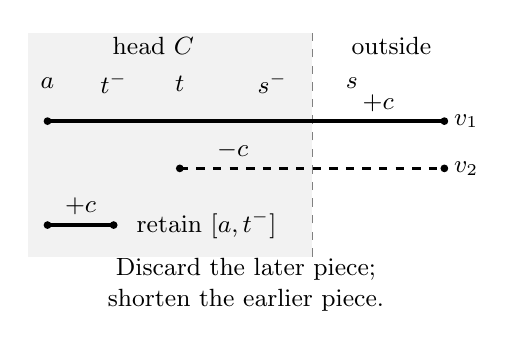
\begin{tikzpicture}[x=0.84cm,y=0.8cm,font=\small]
 \fill[black!5] (-0.3,0.25) rectangle (4,3.8);
 \draw[dashed,gray] (4,0.25)--(4,3.8);
 \node at (1.6,3.6) {head $C$};
 \node at (5.2,3.6) {outside};
 \foreach \x/\name in {0/a,1/{t^-},2/t,3.4/{s^-},4.6/s}
  {\node at (\x,3.0) {$\name$};}
 \draw[very thick] (0,2.4)--(6,2.4);
 \fill (0,2.4) circle (1.4pt); \fill (6,2.4) circle (1.4pt);
 \node[above] at (5,2.4) {$+c$};
 \node[right] at (6,2.4) {$v_1$};
 \draw[very thick,dashed] (2,1.65)--(6,1.65);
 \fill (2,1.65) circle (1.4pt); \fill (6,1.65) circle (1.4pt);
 \node[above] at (2.8,1.65) {$-c$};
 \node[right] at (6,1.65) {$v_2$};
 \draw[very thick] (0,0.75)--(1,0.75);
 \fill (0,0.75) circle (1.4pt); \fill (1,0.75) circle (1.4pt);
 \node[above] at (0.5,0.75) {$+c$};
 \node[right,align=left] at (1.2,0.75) {retain $[a,t^-]$};
 \node[align=center] at (3,-0.2) {Discard the later piece;\\shorten the earlier piece.};
\end{tikzpicture}
\end{minipage}\hfill
\begin{minipage}[t]{0.48\textwidth}
\centering
\textbf{(b) Recover one exterior piece}\par\smallskip
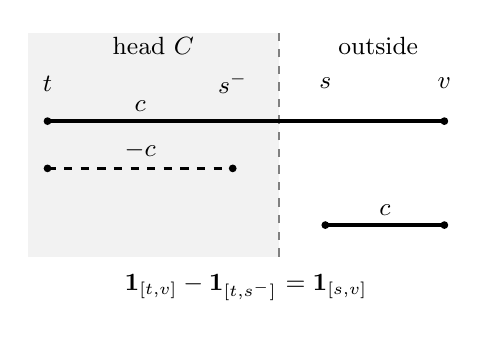
\begin{tikzpicture}[x=0.84cm,y=0.8cm,font=\small]
 \fill[black!5] (-0.3,0.25) rectangle (3.5,3.8);
 \draw[dashed,gray] (3.5,0.25)--(3.5,3.8);
 \node at (1.6,3.6) {head $C$};
 \node at (5.0,3.6) {outside};
 \foreach \x/\name in {0/t,2.8/{s^-},4.2/s,6/v}
  {\node at (\x,3.0) {$\name$};}
 \draw[very thick] (0,2.4)--(6,2.4);
 \fill (0,2.4) circle (1.4pt); \fill (6,2.4) circle (1.4pt);
 \node[above] at (1.4,2.4) {$c$};
 \draw[very thick,dashed] (0,1.65)--(2.8,1.65);
 \fill (0,1.65) circle (1.4pt); \fill (2.8,1.65) circle (1.4pt);
 \node[above] at (1.4,1.65) {$-c$};
 \draw[very thick] (4.2,0.75)--(6,0.75);
 \fill (4.2,0.75) circle (1.4pt); \fill (6,0.75) circle (1.4pt);
 \node[above] at (5.1,0.75) {$c$};
 \node[align=center] at (3,-0.2) {$\mathbf1_{[t,v]}-\mathbf1_{[t,s^-]}$
  \strut$=\mathbf1_{[s,v]}$};
\end{tikzpicture}
\end{minipage}
\caption{Segment matching in the representative case
$a\prec t\preceq s^-$, where $a$ and $t$ are the earlier and later
starts and $s$ is the first node outside the head. Each row represents
a segment; its labels through $s$ refer to the common ancestor chain.
In (a), the displayed signs are opposite coefficient signs, with
$c>0$; they are independent of the $+$ and $-$ endpoint-origin labels.
In (b), a piece from the $+$ endpoint can have either sign of $c$.
Its exterior is reproduced using at most two segments starting at $t$.
The proof also covers coincident starts, $t=s$, and roots outside $C$.}
\label{fig:segment-matching}
\end{figure}

\begin{proof}
Fix $\eta>0$ and put
$R=\max\{\|p+y\|_S,\|p-y\|_S\}+\eta$. Choose representations of $p+y$
and $p-y$ of cost at most $R$. Halve every coefficient and concatenate
the two lists, retaining the labels $+$ and $-$ that record their
origins. These labels are independent of the signs of the coefficients.
The combined list has output $p$ and start mass $m$ with $M(m)\le R$.
Figure~\ref{fig:segment-matching} illustrates the two uses of a matched pair.

A first node outside $C$ means a node $s\notin C$ whose parent lies in
$C$, or a root outside $C$. Every segment is then of exactly one of
three kinds: it lies wholly in $C$; it contains one first node outside
$C$; or its start lies strictly below a first node outside $C$.
The second kind includes segments starting at that first node.
At each such $s$, match the positive and
negative weights of all segments containing $s$ in pieces of equal
absolute weight. Their total positive and total negative masses are
finite and equal, since their sum is the output $p_s=0$. For completeness,
place the positive weights consecutively on an interval of their total
length, do the same with the absolute negative weights, and use the
intersections of these intervals as matching pieces. This produces a
countable matching that uses every weight. A segment contains at most
one first node outside $C$, so the matchings do not interfere.

In each matched pair, both starts are ancestors of its first outside
node $s$. Call the piece with deeper start the later piece, breaking a
tie arbitrarily. Define $r_t$ to be the sum of the sizes of later pieces
starting at $t$, together with the sizes of all original pieces starting
strictly below a first node outside $C$. These are disjoint portions of
the list; hence $0\le r\le m$.

We first recover $p$ at cost at most $M(m-r)$. Delete all pieces starting
strictly below a first outside node. For a matched pair with coincident
starts, discard both pieces. Otherwise discard the later piece and
shorten the earlier piece to end immediately before the later start.
The remaining part
lies in $C$. On $C$ the removed overlapping parts had equal opposite
coefficients and therefore canceled. Segments wholly inside $C$ are
unchanged. The modified list consequently represents $p$, and its start
masses are at most $m-r$. By~\eqref{sm:s:positive-energy},
\begin{equation}\label{sm:s:saved-mass}
 \|p\|_S^2+M(r)^2\le M(m-r)^2+M(r)^2\le M(m)^2.
\end{equation}

It remains to control $y$ by the saved mass. The output of the $+$ list
outside $C$ is $y/2$. We represent it using start masses at most $4r$.
Include each $+$ piece starting strictly below a first outside node
without change. For a $+$ piece in a pair at $s$, let $t$ be the pair's
later start and $v$ the endpoint of this piece. Replace its exterior part
by the segment $[t,v]$ with its original coefficient. If $t\in C$, also
include the segment from $t$ to the parent of $s$ with the opposite
coefficient. These two segments leave precisely the desired output
from $s$ to $v$. If $t=s$, no subtraction is needed. Each pair has at most
two $+$ pieces, and each uses at most two segments of the matched size,
all starting at $t$. Their total start mass is therefore at most four
times the later piece's mass. No segment wholly in $C$ is needed. Thus
\begin{equation}\label{sm:s:tail-recovery}
 \|y\|_S\le2M(4r)=8M(r).
\end{equation}

All the modified lists are legitimate: their absolute start masses have
finite cost, and each coordinate has only finitely many ancestors.
Combining~\eqref{sm:s:saved-mass} and~\eqref{sm:s:tail-recovery} gives
$\|p\|_S^2+\|y\|_S^2/64\le R^2$. Finally let $\eta\downarrow0$.
\end{proof}

\begin{corollary}\label{sm:s:midpoint-consequence}
For every $x\in X_S$ with $\|x\|_S=1$, every $t>0$ and every $\varepsilon>0$
there is a closed finite-codimensional subspace $F\subset X_S$ such that
\[
 \inf_{\substack{y\in F\\\|y\|_S=1}}
 \max\{\|x+ty\|_S,\|x-ty\|_S\}
 \ge\sqrt{1+t^2/64}-\varepsilon.
\]
In particular, define the maximum form of the asymptotic midpoint modulus
by
\[
 \delta^{\max}_{X_S}(t)=
 \inf_{\|x\|_S=1}\sup_{\substack{F\subset X_S\text{ closed}\\\dim(X_S/F)<\infty}}
 \inf_{\substack{y\in F\\\|y\|_S\ge1}}
 \bigl(\max_{\pm}\|x\pm ty\|_S-1\bigr).
\]
Then $\delta^{\max}_{X_S}(t)\ge\sqrt{1+t^2/64}-1$.
\end{corollary}
\begin{proof}
Choose a finite-support $p$ arbitrarily close to $x$, let $C$ be its finite
ancestral closure and set $F=\ker P_C$. Theorem~\ref{thm:segment-start-tail}
gives, uniformly for $y\in F$ with $\|y\|_S\ge1$,
\[
 \max_{\pm}\|x\pm ty\|_S
 \ge\sqrt{\|p\|_S^2+t^2/64}-\|x-p\|_S.
\]
As $\|x-p\|_S\to0$, the right side tends to
$\sqrt{1+t^2/64}$. Coordinate continuity makes $F$ closed and
finite-codimensional, proving the assertion.
\end{proof}

\section{Incomparable segments}
\label{sm:i:section}

In this section, arrays are tested by families of segments in which every
node of one segment is incomparable with every node of another.  The resulting dual space has unit root paths of
arbitrarily large finite height. When both endpoints lie in the unit ball,
a midpoint close to the unit sphere forces small displacement beyond any
finite prefix supporting that midpoint. We prove the latter assertion by replacing the
coefficients of segment atoms with the sums of a norming test along their
segments.  Opposite signs can then be controlled by shortening segments
without violating their incomparability.

\subsection{The norm and its dual atoms}

For an integer $h\geq1$, let $T_h=\mathbb N^{\leq h}$, including the empty
sequence as its root, and take disjoint copies when forming
$\mathcal T=\bigsqcup_{h\geq1}T_h$.
Nodes in the same tree are ordered by extension, denoted by $s\preceq t$;
nodes in different trees are incomparable.  If $s\preceq t$, the segment
$[s,t]$ consists of every node between $s$ and $t$, including both
endpoints.  A finite family $(S_i)_{i=1}^m$ of nonempty segments is
\emph{incomparable} if, for $i\ne j$, every node of $S_i$ is incomparable
with every node of $S_j$.  In particular, the segments are disjoint, but
disjointness alone is not this condition.

For a finitely supported real array $g$ on $\mathcal T$, set
\begin{equation}
 \|g\|_{Y_{\mathrm I}}
 =\sup_{(S_i)\text{ incomparable}}
   \left(\sum_{i=1}^m
     \left|\sum_{v\in S_i}g(v)\right|^2\right)^{1/2},
 \label{sm:i:norm}
\end{equation}
and let $Y_{\mathrm I}$ be its completion.  This is a finite norm on
$c_{00}(\mathcal T)$: the triangle inequality follows from the Euclidean
triangle inequality, singleton tests separate points, and disjointness
bounds every test by $\sum_v|g(v)|$.
Each coordinate and each finite segment evaluation extends continuously
to $Y_{\mathrm I}$.  Formula~\eqref{sm:i:norm} remains valid in the
completion.  Indeed, the supremum of the extended tests is at most the
completion norm and is Lipschitz with constant one; approximation by
finitely supported arrays gives the reverse inequality.

Quadratic aggregation over incomparable segment families also appears
in the $\ell_2$-Baire-sum construction of Argyros and Dodos
\cite[author version, Section~4.1]{ArgyrosDodos2007}. There each segment
contributes the norm of a sum in a Schauder tree basis; here it contributes
the absolute scalar sum in~\eqref{sm:i:norm}.

\begin{proposition}\label{sm:i:reflexivity}
Let $Y_{\mathrm I,h}$ be the completion of the arrays supported on $T_h$
in the norm~\eqref{sm:i:norm}.  Then
\begin{equation}
 \frac{\|g\|_2}{\sqrt{h+1}}
 \leq\|g\|_{Y_{\mathrm I,h}}
 \leq\sqrt{h+1}\,\|g\|_2,
 \qquad g\in c_{00}(T_h),
 \label{sm:i:hilbert}
\end{equation}
and
\[
 Y_{\mathrm I}=\left(\bigoplus_{h\geq1}Y_{\mathrm I,h}\right)_{\ell_2}.
\]
Both $Y_{\mathrm I}$ and $X_{\mathrm I}:=Y_{\mathrm I}^*$ are reflexive.
\end{proposition}

\begin{proof}
At each fixed level of $T_h$, the singleton segments form an incomparable
family.  Hence the squared norm of $g$ dominates the sum of $|g(v)|^2$
over that level.  Summing over the $h+1$ levels gives the lower bound
in~\eqref{sm:i:hilbert}.  For the upper bound, every segment has at most
$h+1$ nodes, so Cauchy--Schwarz and disjointness give
\[
 \sum_i\left|\sum_{v\in S_i}g(v)\right|^2
 \leq(h+1)\sum_i\sum_{v\in S_i}|g(v)|^2
 \leq(h+1)\|g\|_2^2.
\]
Thus $Y_{\mathrm I,h}$ is isomorphic to the Hilbert space $\ell_2(T_h)$
and is reflexive.

A test family separates into families on the individual trees.  Conversely,
the union of finitely many such families, one in each of distinct trees,
is incomparable.  Choosing each component family arbitrarily close to
its supremum proves
\[
 \|g\|_{Y_{\mathrm I}}^2
 =\sum_h\|g|_{T_h}\|_{Y_{\mathrm I,h}}^2
\]
for finitely supported $g$, and then the asserted sum decomposition
follows by completion.
For completeness, the dual of an $\ell_2$-sum of Banach spaces is the
$\ell_2$-sum of their duals: Cauchy--Schwarz bounds the sum of the
pairings, while finitely many nearly norming component vectors with
suitable scalar weights give the opposite norm inequality.  Restrictions
to the components determine a functional by density.  Applying this
description twice, componentwise reflexivity shows that the canonical
map into the bidual is onto.  Thus $Y_{\mathrm I}$ is reflexive, as is
its dual $X_{\mathrm I}$.
\end{proof}

Write $e_v\in X_{\mathrm I}$ for evaluation at $v$, and put
$z_S=\sum_{v\in S}e_v$, with $z_\varnothing=0$.  We denote the dual norm
by $\|\cdot\|_{\mathrm I}$.  The coordinate evaluations are linearly
independent, so $X_{\mathrm I}$ is infinite dimensional.  An \emph{atom}
is a vector together with a representation
\begin{equation}
 A=\sum_{i=1}^m a_i z_{S_i},
 \qquad \sum_{i=1}^m a_i^2\leq1,
 \qquad (S_i)_{i=1}^m\text{ incomparable}.
 \label{sm:i:atoms}
\end{equation}
The representation will matter when its coefficients are replaced below.

\begin{lemma}\label{sm:i:atom-hull}
The unit ball of $X_{\mathrm I}$ is the norm-closed convex hull of the
atoms~\eqref{sm:i:atoms}.  In particular, finite linear combinations of
the coordinate evaluations are dense in $X_{\mathrm I}$.
\end{lemma}

\begin{proof}
Every atom has norm at most one, by Cauchy--Schwarz
and~\eqref{sm:i:norm}, and for every $g\in Y_{\mathrm I}$,
\[
 \sup_{A\text{ atom}} A(g)=\|g\|_{Y_{\mathrm I}}.
\]
If the closed convex hull of the atoms missed a point of the dual unit
ball, Hahn--Banach separation would give a separating functional in
$X_{\mathrm I}^*=Y_{\mathrm I}$, using Proposition~\ref{sm:i:reflexivity}.
The displayed identity rules out such a separation.  Each atom has
finite support, which gives the density assertion.
\end{proof}

\subsection{Unit paths and finite prefixes}

The root paths give the one-sided obstruction; finite prefixes will
separate the head of a midpoint from its remaining coordinates.
For $s\in T_h$, define
\[
 v_s=z_{[\varnothing_h,s]},
\]
where $\varnothing_h$ denotes the root of that copy of $T_h$.
Each $v_s$ is an atom of norm one: its norm is at most one by
Lemma~\ref{sm:i:atom-hull}, and testing it against the array which equals
one at $s$ and zero elsewhere gives the reverse inequality.  The same
argument gives $\|e_t\|_{\mathrm I}=1$ for every node $t$.
If $|s|<h$ and $t_j=s^\frown j$, then
\begin{equation}
 v_{t_j}=v_s+e_{t_j},\qquad
 \|v_s\|_{\mathrm I}=\|e_{t_j}\|_{\mathrm I}=1,
 \qquad e_{t_j}\longrightarrow0\text{ weakly}.
 \label{sm:i:paths}
\end{equation}
To verify weak convergence, singleton tests at the children show that
$\sum_j|g(t_j)|^2\leq\|g\|_{Y_{\mathrm I}}^2$ for each
$g\in Y_{\mathrm I}$.  Thus $g(t_j)\to0$, and these are all the
functionals on $X_{\mathrm I}$ by reflexivity.

\begin{corollary}\label{sm:i:auc-obstruction}
The real reflexive space $X_{\mathrm I}$ admits no equivalent
asymptotically uniformly convex norm.
\end{corollary}

\begin{proof}
The trees~\eqref{sm:i:paths} exist at every finite height and satisfy
Lemma~\ref{lem:bounded-tree} with path bounds and increment lower bound
all equal to one.  More explicitly, for an equivalent norm $N$ with
$a\|u\|_{\mathrm I}\leq N(u)\leq b\|u\|_{\mathrm I}$, that lemma
uses $t_0=a/(2b)$.  If
$\delta=\overline\delta_N(t_0)>0$, its finite-codimensional approximation
and convexity argument selects a child at every nonterminal node for
which
\[
 N(v_{t_j})\geq (1+\delta/4)N(v_s).
\]
Iteration to height $h$ gives
$a(1+\delta/4)^h\leq b$, a contradiction for sufficiently large $h$.
\end{proof}

A set $E\subset\mathcal T$ is \emph{prefix closed} if it contains every
ancestor of each of its nodes, within that node's tree.  Let $P_E$ be
coordinate restriction to $E$, and let $Q_E=I-P_E$.

\begin{lemma}\label{sm:i:projections}
For every finite prefix-closed $E$, both $P_E$ and $Q_E$ act
contractively on $Y_{\mathrm I}$ and, by adjoints, on $X_{\mathrm I}$.
On $X_{\mathrm I}$, $P_E$ has finite rank and retains exactly the
coordinates indexed by $E$.  For every $x\in X_{\mathrm I}$ and every
$\eta>0$, there is such an $E$ with $\|Q_E x\|_{\mathrm I}<\eta$.
\end{lemma}

\begin{proof}
The nonempty intersections of an incomparable segment family with $E$
are again incomparable segments; the same is true of the portions
outside $E$.  Here prefix closure ensures that a segment is cut into
an initial part and a terminal part.  Applying these restricted tests to
the original array proves both contraction inequalities on
$Y_{\mathrm I}$, first on finite arrays and then on the completion.
The adjoints are contractions and act as the stated coordinate
projections on each $e_v$, hence on $X_{\mathrm I}$ by
Lemma~\ref{sm:i:atom-hull}.  The range of $P_E$ is contained in the span
of the finitely many $e_v$ with $v\in E$.
Finally, approximate $x$ by a finitely supported vector and let $E$
contain its support and all its ancestors.  The contraction bound for
$Q_E$ gives the last assertion.
\end{proof}

\subsection{Replacing coefficients and controlling cancellation}

The following estimate is uniform in the finite prefix and allows an
arbitrary displacement.  Its tail-supported case is the symmetric
splitting estimate for this model.

\begin{theorem}\label{sm:i:tail-estimate}
Let $E\subset\mathcal T$ be finite and prefix closed.  If
$x,y\in X_{\mathrm I}$ satisfy
\[
 P_E x=x,\qquad \|x+y\|_{\mathrm I}\leq1,
 \qquad \|x-y\|_{\mathrm I}\leq1,
\]
then
\begin{equation}
 \|Q_Ey\|_{\mathrm I}
 \leq (\sqrt2+\sqrt6)\sqrt{1-\|x\|_{\mathrm I}}.
 \label{sm:i:tail-bound}
\end{equation}
In particular, if $Q_Ey=y$, the same bound holds for $\|y\|_{\mathrm I}$.
\end{theorem}

\begin{proof}
Convexity gives $\|x\|_{\mathrm I}\leq1$.
Choose $f\in Y_{\mathrm I}$ supported on $E$ such that
\[
 \|f\|_{Y_{\mathrm I}}\leq1,
 \qquad x(f)=\|x\|_{\mathrm I}.
\]
Indeed, Hahn--Banach gives a norming element of $X_{\mathrm I}^*$;
reflexivity identifies it with an element of $Y_{\mathrm I}$, and
applying $P_E$ preserves its pairing with $x$ without increasing its
norm.  If $x=0$, we may simply take $f=0$.

For an atom with representation~\eqref{sm:i:atoms}, define
\[
 p_i^A=z_{S_i}(f),\qquad
 d(A)=1-A(f)=1-\sum_i a_i p_i^A\geq0.
\]
Both coefficient vectors $(a_i)$ and $(p_i^A)$ have Euclidean norm at
most one.  The identity
\[
 2d(A)=\sum_i(a_i-p_i^A)^2
       +\left(1-\sum_i a_i^2\right)
       +\left(1-\sum_i(p_i^A)^2\right)
\]
therefore gives
\begin{equation}
 \sum_i(a_i-p_i^A)^2\leq2d(A),
 \qquad 1-\sum_i(p_i^A)^2\leq2d(A).
 \label{sm:i:defect}
\end{equation}
Replace the coefficients on the terminal pieces by setting
\[
 \widehat A=\sum_i p_i^A z_{S_i\setminus E}.
\]
Those nonempty terminal pieces remain incomparable.  The atom norm
bound and~\eqref{sm:i:defect} imply
\begin{equation}
 \|\widehat A-Q_EA\|_{\mathrm I}\leq\sqrt{2d(A)}.
 \label{sm:i:replacement}
\end{equation}

Let $\mathcal R$ be the minimal nodes of $\mathcal T\setminus E$.
They form an antichain and their descendant subtrees partition the
complement.  If $p_i^A\ne0$ and $S_i\setminus E$ is nonempty, the original segment
meets $E$ and exits it through exactly one $q\in\mathcal R$.
For a fixed $q$, at most one segment in an incomparable family can do
this, since two such segments would both contain $q$.  We may write
\begin{equation}
 \widehat A=\sum_{q\in\mathcal R}r_q^A z_{[q,t_q^A]}.
 \label{sm:i:exits}
\end{equation}
Only finitely many coefficients are nonzero.  When $r_q^A\ne0$, let
$s_q^A\in E$ be the starting node of the original segment and let
$t_q^A\succeq q$ be its terminal node.  Then $r_q^A$ is the sum of $f$
from $s_q^A$ to the predecessor of $q$.  For zero coefficients choose
$t_q^A=q$; no starting node is needed.

We next show that opposite coefficients in two atoms consume their
norming defects:
\begin{equation}
 \sum_{q:\,r_q^Ar_q^{A'}<0}|r_q^Ar_q^{A'}|
 \leq \frac12\left(1-\sum_i(p_i^A)^2
                  +1-\sum_i(p_i^{A'})^2\right)
 \leq d(A)+d(A').
 \label{sm:i:cancellation}
\end{equation}
For any exit occurring in this sum, the two starting nodes lie on the
same ancestor path of $q$.  They are distinct, since identical starts
would give identical sums of $f$, rather than opposite signs.
Consider first the exits for which $s_q^A\prec s_q^{A'}$.
Shorten the corresponding segment of $A$ to the interval from $s_q^A$
to the predecessor of $s_q^{A'}$.  This interval is nonempty and is a
subsegment of the original segment.  Distinct exits correspond to
distinct segments, so all these shortenings can be made simultaneously.
Every modified family is still incomparable.  Its corresponding
squared evaluation changes from $(r_q^A)^2$ to
$(r_q^A-r_q^{A'})^2$, an increase of
\[
 (r_q^{A'})^2+2|r_q^Ar_q^{A'}|
 \geq2|r_q^Ar_q^{A'}|.
\]
All its squared evaluations sum to at most one.  Thus the sum of these
products is at most $\tfrac12(1-\sum_i(p_i^A)^2)$.
For the exits with the opposite ordering, shorten the segments of $A'$
instead and obtain the other half of~\eqref{sm:i:cancellation}.
The final inequality follows from~\eqref{sm:i:defect}.

We have controlled the replacement error for one atom and opposite
exit coefficients for two atoms.  It remains to apply these facts to
convex combinations approximating the two endpoints $x+y$ and $x-y$.
Fix $\varepsilon>0$.  By Lemma~\ref{sm:i:atom-hull}, choose a finite
probability distribution of atoms for each endpoint whose mean differs
from that endpoint in norm by at most $\varepsilon$.  Choose
$\sigma\in\{-1,1\}$ with equal probabilities, then choose $A$ from the
distribution for $x+\sigma y$.  Consequently
\[
 \|\mathbb E A-x\|_{\mathrm I}\leq\varepsilon,
 \qquad
 \|\mathbb E(\sigma A)-y\|_{\mathrm I}\leq\varepsilon,
 \qquad
 0\leq\bar d:=\mathbb E d(A)
 \leq1-\|x\|_{\mathrm I}+\varepsilon.
\]
Contractivity of $Q_E$, the identity $Q_Ex=0$, and
Cauchy--Schwarz applied to~\eqref{sm:i:replacement} give
\begin{equation}
 \|\mathbb E\widehat A\|_{\mathrm I}
 \leq\varepsilon+\sqrt{2\bar d},
 \qquad
 \|\mathbb E(\sigma\widehat A)-Q_Ey\|_{\mathrm I}
 \leq\varepsilon+\sqrt{2\bar d}.
 \label{sm:i:mixture-errors}
\end{equation}

Put $m_q=\mathbb E r_q^A$ and $b_q=\mathbb E|r_q^A|$.
Apply~\eqref{sm:i:cancellation} to independent copies $A,A'$ of the
unconditional atom distribution.  With $r_+=\max(r,0)$ and
$r_-=\max(-r,0)$, independence gives
\[
 2\sum_q\mathbb E[(r_q^A)_+]\,\mathbb E[(r_q^A)_-]
 \leq2\bar d.
\]
Since $b_q^2-m_q^2=4\mathbb E[(r_q^A)_+]\,\mathbb E[(r_q^A)_-]$,
\begin{equation}
 \sum_q b_q^2\leq\sum_qm_q^2+4\bar d.
 \label{sm:i:unsigned-mass}
\end{equation}
At this fixed $\varepsilon$, the distributions are finite and their
atoms have finite support.  Thus all sums of $m_q$ and $b_q$ above are
finite, even though $\mathcal R$ can be infinite.

An array supported on the antichain $\mathcal R$ has
$Y_{\mathrm I}$-norm equal to its Euclidean norm: a segment meets at
most one of its support nodes, and singleton segments realize the
Euclidean test.  The coefficient of $\mathbb E\widehat A$ at $q$ is
$m_q$, so duality gives
\begin{equation}
 \left(\sum_qm_q^2\right)^{1/2}
 \leq\|\mathbb E\widehat A\|_{\mathrm I}.
 \label{sm:i:signed-mass}
\end{equation}
For $g\in Y_{\mathrm I}$ with $\|g\|_{Y_{\mathrm I}}\leq1$, define
\[
 L_q=\sup_{t\succeq q}|z_{[q,t]}(g)|.
\]
For each finite subset of exits, choose segments approaching these
suprema.  The chosen segments are incomparable, so their squared
evaluations sum to at most one.  Passing to the suprema and then taking
the supremum over finite subsets proves $\sum_qL_q^2\leq1$;
no supremum need be attained.  It follows that
\[
 |\mathbb E(\sigma\widehat A)(g)|
 \leq\sum_qb_qL_q
 \leq\left(\sum_qb_q^2\right)^{1/2}.
\]
Taking the supremum over $g$, and
using~\eqref{sm:i:mixture-errors}--\eqref{sm:i:signed-mass}, yields
\[
 \|Q_Ey\|_{\mathrm I}
 \leq\varepsilon+\sqrt{2\bar d}
   +\left((\varepsilon+\sqrt{2\bar d})^2+4\bar d\right)^{1/2}.
\]
The right-hand side is increasing in $\bar d$.  Substitute
$\bar d\leq1-\|x\|_{\mathrm I}+\varepsilon$ and let
$\varepsilon\downarrow0$.  The two limiting contributions are
$\sqrt{2(1-\|x\|_{\mathrm I})}$ and
$\sqrt{6(1-\|x\|_{\mathrm I})}$, proving~\eqref{sm:i:tail-bound}.
\end{proof}

\subsection{Separated midpoint families}

The next corollary removes the finite-prefix condition on the center:
if $x\pm u_j$ lie in the unit ball for an infinite separated family
$(u_j)$, then the norm of the common midpoint $x$ is bounded away from one.

\begin{corollary}\label{sm:i:separated-midpoints}
Let $0<c\leq1$ and let $x,u_j\in X_{\mathrm I}$, $j\in\mathbb N$,
satisfy
\[
 \|x+u_j\|_{\mathrm I},\ \|x-u_j\|_{\mathrm I}\leq1,
 \qquad \|u_j-u_k\|_{\mathrm I}\geq2c\quad(j\ne k).
\]
Then, with $K=\sqrt2+\sqrt6$,
\begin{equation}
 \|x\|_{\mathrm I}\leq1-(c/K)^2<1.
 \label{sm:i:separation-bound}
\end{equation}
\end{corollary}

\begin{proof}
Fix $0<\eta<c$ and use Lemma~\ref{sm:i:projections} to choose $E$ with
$\|Q_Ex\|_{\mathrm I}<\eta$.  The sequence $(u_j)$ is bounded, since
$u_j=((x+u_j)-(x-u_j))/2$.  The range of $P_E$ is finite dimensional,
so there are distinct $j,k$ such that, for
$w=(u_j-u_k)/2$, one has $\|P_Ew\|_{\mathrm I}<\eta$.
The separation assumption gives $\|w\|_{\mathrm I}\geq c$.
Moreover, $x+w$ is the midpoint of $x+u_j$ and $x-u_k$, and $x-w$ is
the midpoint of the other two endpoints.  Hence
$\|x\pm w\|_{\mathrm I}\leq1$.  Therefore
\[
 \|P_Ex\pm Q_Ew\|_{\mathrm I}\leq1+2\eta,
 \qquad \|Q_Ew\|_{\mathrm I}\geq c-\eta.
\]
Apply Theorem~\ref{sm:i:tail-estimate} after dividing both vectors by
$1+2\eta$:
\[
 \frac{c-\eta}{1+2\eta}
 \leq K\sqrt{1-\frac{\|P_Ex\|_{\mathrm I}}{1+2\eta}}.
\]
Since $\|P_Ex-x\|_{\mathrm I}<\eta$, letting $\eta\downarrow0$ gives
$ c\leq K\sqrt{1-\|x\|_{\mathrm I}}$, which is
\eqref{sm:i:separation-bound}.
\end{proof}

\bibliographystyle{plain}
\bibliography{references}
\end{document}
